\documentclass[12pt,a4paper]{report}

\usepackage[top=2.5cm, bottom=2.5cm, left=3.5cm, right=2.5cm]{geometry}
\usepackage{setspace}
\setstretch{1.3}
\setlength{\parskip}{2.5pt}
\setlength{\parindent}{1.0cm}
\widowpenalty=10000
\clubpenalty=10000
\usepackage{amsmath}
\usepackage{amssymb}
\usepackage{amsfonts}
\usepackage{algorithm}
\usepackage{algpseudocode}
\floatname{algorithm}{Thuật toán}
\numberwithin{algorithm}{chapter}
\newcounter{lemma}[chapter]
\renewcommand{\thelemma}{\thechapter.\arabic{lemma}}
\newcounter{theorem}[chapter]
\renewcommand{\thetheorem}{\thechapter.\arabic{theorem}}
\newcounter{corollary}[chapter]
\renewcommand{\thecorollary}{\thechapter.\arabic{corollary}}
\renewcommand{\algorithmicrequire}{\textbf{Đầu vào:}}
\renewcommand{\algorithmicensure}{\textbf{Đầu ra:}}
\usepackage{fontspec}
\setmainfont{Times New Roman}
\setmonofont{Consolas}[Scale=MatchLowercase]
\usepackage{graphicx}
\graphicspath{{../}}
\usepackage{float}
\usepackage{placeins}
\usepackage{fancybox}
\usepackage{array}
\usepackage{booktabs}
\usepackage{longtable}
\usepackage{tabularx}
\usepackage{enumitem}
\usepackage{xcolor}
\usepackage{hyperref}
\usepackage{fancyhdr}
\usepackage{titlesec}

% Cấu hình tiêu đề theo Phong cách Tối giản 1 dòng (Lựa chọn 4: One-Line Minimalist)
\titleformat{\chapter}[hang]
    {\normalfont\Large\bfseries}
    {\thechapter.\quad}
    {0pt}
    {}
\titlespacing*{\chapter}
    {0pt}
    {-30pt}
    {15pt}

\titleformat{\section}[hang]
    {\normalfont\large\bfseries}
    {\thesection\quad}
    {0pt}
    {}
\titlespacing*{\section}
    {0pt}
    {12pt}
    {6pt}

\titleformat{\subsection}[hang]
    {\normalfont\normalsize\bfseries}
    {\thesubsection\quad}
    {0pt}
    {}
\titlespacing*{\subsection}
    {0pt}
    {10pt}
    {4pt}
\usepackage{tikz}
\usetikzlibrary{
    arrows.meta,
    backgrounds,
    calc,
    fit,
    positioning,
    shapes.geometric,
    shapes.multipart
}

\renewcommand{\contentsname}{Mục lục}
\renewcommand{\listfigurename}{Danh mục hình vẽ}
\renewcommand{\listtablename}{Danh mục bảng}
\renewcommand{\chaptername}{Chương}
\renewcommand{\figurename}{Hình}
\renewcommand{\tablename}{Bảng}
\renewcommand{\bibname}{Tài liệu tham khảo}

\hypersetup{
    colorlinks=true,
    linkcolor=black,
    urlcolor=black,
    citecolor=black
}
\urlstyle{same}

\setlist[itemize]{leftmargin=1.0cm, itemsep=2pt, topsep=2pt, parsep=0pt}
\setlist[enumerate]{leftmargin=1.0cm, itemsep=2pt, topsep=2pt, parsep=0pt}
\renewcommand{\arraystretch}{1.25}
\setlength{\tabcolsep}{3pt}
\newcolumntype{L}[1]{>{\raggedright\hspace{0pt}\arraybackslash}p{#1}}
\newcolumntype{Y}{>{\raggedright\hspace{0pt}\arraybackslash}X}
\newcommand{\code}[1]{{\ttfamily\urlstyle{same}\nolinkurl{#1}}}

\pagestyle{fancy}
\fancyhf{}
\fancyhead[L]{Đồ án liên ngành - RareProtSelect}
\fancyfoot[C]{\thepage}
\renewcommand{\headrulewidth}{0.4pt}
\fancypagestyle{plain}{
    \fancyhf{}
    \fancyhead[L]{Đồ án liên ngành - RareProtSelect}
    \fancyfoot[C]{\thepage}
    \renewcommand{\headrulewidth}{0.4pt}
}
\setlength{\headheight}{16.5pt}
\emergencystretch=3em
\hyphenation{RareProtSelect Subfamily Subfamilies Peptidase Peptidases Facility Location BLASTp}
\renewcommand{\topfraction}{0.90}
\renewcommand{\bottomfraction}{0.80}
\renewcommand{\textfraction}{0.07}
\renewcommand{\floatpagefraction}{0.85}
\setcounter{topnumber}{3}
\setcounter{bottomnumber}{2}
\setcounter{totalnumber}{4}

\begin{document}

\pagenumbering{gobble}
\thisfancypage{\setlength{\fboxsep}{0.2cm}\setlength{\fboxrule}{1pt}\doublebox}{}
\begin{titlepage}
    \begin{center}
        \large
        \textbf{BỘ GIÁO DỤC VÀ ĐÀO TẠO}\\
        \textbf{ĐẠI HỌC PHENIKAA}\\
        \vspace{-0.9em}
        \rule{3cm}{0.4pt}
    \end{center}

    \begin{figure}[H]
        \centering
        
\includegraphics[width=0.68\textwidth]{Images/pnk_logo.jpg}
    \end{figure}

    \begin{center}
        {\huge\textbf{BÁO CÁO ĐỒ ÁN LIÊN NGÀNH}}
    \end{center}

    \begin{center}
        {\Large\textbf{HỌC PHẦN: ĐỒ ÁN LIÊN NGÀNH\\KHOA HỌC MÁY TÍNH}\par}
    \end{center}

    \begin{center}
        {\Large\textbf{ĐỀ TÀI:}\par}
        \vspace{0.3cm}
        {\Large\textbf{CHỌN TẬP PROTEIN ĐẠI DIỆN\\CÓ ƯU TIÊN NHÓM HIẾM\\BẰNG TỐI ƯU HÓA SUBMODULAR}\par}

        \vspace{1.6cm}
        \begin{tabular}{l l}
            \textbf{Sinh viên thực hiện:} & Đoàn Anh Hùng -- 23010022 \\
                                          & Vũ Trường Giang -- 23010257 \\
                                          & Nguyễn Quang Hiệp -- 23010451 \\[0.5em]
            \textbf{Giảng viên hướng dẫn:} & TS. Trần Đình Tân
        \end{tabular}
    \end{center}

    \vspace*{\fill}
    \begin{center}
        \textbf{HÀ NỘI, 2026}
    \end{center}
\end{titlepage}

\clearpage

\pagenumbering{roman}
\chapter*{Tóm tắt}
\phantomsection
\addcontentsline{toc}{chapter}{Tóm tắt}

Chọn tập chuỗi protein đại diện có kiểm soát ngân sách là bài toán tiền xử lý quan trọng trong tin sinh học phân tử nhằm giảm chi phí tính toán cho so khớp đa chuỗi và phân tích tiến hóa. Thách thức lớn nhất là phân bố mất cân bằng lớn về quy mô theo quy luật đuôi dài trong các siêu họ enzyme tự nhiên, điển hình tại siêu họ Peptidase A1 trong cơ sở dữ liệu MEROPS~\cite{merops} với tập dữ liệu gồm $4.120$ chuỗi thuộc $115$ Subfamily chính thức sau khi loại bỏ các chuỗi chưa phân loại. Các công cụ gom cụm truyền thống như CD-HIT~\cite{cdhit} hay MMseqs2~\cite{mmseqs2} không thể kiểm soát trực tiếp số lượng chuỗi đại diện. Trong khi đó, mô hình submodular Facility Location không trọng số~\cite{nguyen2025} dồn ngân sách vào các phân họ lớn, bỏ sót hơn một nửa số Subfamily ở mức $0\%$ Sensitivity và gây sai lệch bao phủ chéo ngoài ranh giới phân họ.

Đồ án đề xuất khung phương pháp luận RareProtSelect gồm ba đóng góp cốt lõi. Thứ nhất, thiết lập họ hàm mục tiêu Weighted Facility Location với trọng số nghịch đảo quy mô Subfamily, chứng minh giải tích tính đơn điệu không giảm, tính submodular và thiết lập nền tảng lý thuyết theo cận xấp xỉ $(1 - 1/e)$ của giải thuật tham lam chuẩn~\cite{nemhauser1978}. Thứ hai, hiện thực hóa giải thuật Pruned Greedy trên GPU kết hợp cơ chế xác lập thứ hạng đồng thuận và khung đánh giá nội phân họ Within-Subfamily Coverage nhằm loại bỏ sai lệch bao phủ chéo. Thứ ba, tích hợp module khảo sát mở rộng trên không gian ngữ nghĩa liên tục ESM-2~\cite{esm2} kết hợp kỹ thuật dịch tâm Mean-Centering nhằm khắc phục hiện tượng co cụm vector.

Kết quả từ chuỗi 6 thử nghiệm tuần tự khẳng định tham số $\alpha$ điều khiển trực tiếp sự đánh đổi đa mục tiêu giữa độ bao phủ toàn cục và chỉ số Rare Sensitivity: dù ở vùng ngân sách nhỏ và trung bình ($k < G$) việc ưu tiên nhóm hiếm đòi hỏi giảm một phần chỉ số Overall Sensitivity, tại ngân sách đối chuẩn đầy đủ $k = G = 115$ trên không gian NCBI BLASTp~\cite{blast}, cấu hình trọng số cân bằng $\alpha = 0{,}5$ nâng chỉ số Rare Sensitivity từ $2{,}22\%$ lên $59{,}11\%$, tức tăng gấp $26{,}6$ lần khi cố định ngưỡng ngân sách tối đa $k_{\max} = 115$ và đạt $50{,}22\%$, tức gấp $22{,}6$ lần khi mở rộng ngưỡng ngân sách tối đa lên $k_{\max} = 380$, đồng thời nâng chỉ số Macro-Average Sensitivity từ $49{,}28\%$ lên $78{,}87\%$ mà vẫn duy trì chỉ số Overall Sensitivity ở mức $94{,}13\%$ so với $93{,}57\%$ của mô hình cơ sở không trọng số. Hiệu năng bảo tồn nhóm hiếm cũng được cải thiện trên không gian ngữ nghĩa liên tục ESM-2 ở vùng ngân sách trung bình; đồng thời khi mở rộng ngân sách lên $k = 380$, tập đại diện hội tụ và bao phủ $112$ trên $115$ Subfamily trong siêu họ.

\smallskip

{\raggedright\noindent\textbf{Từ khóa:} chọn tập protein đại diện, tối ưu hóa submodular, Subfamily hiếm, Weighted Facility Location, Within-Subfamily Coverage, mô hình ngôn ngữ protein ESM-2, MEROPS Family A1.\par}

\clearpage


\begingroup
\setstretch{1.06}
\setlength{\parskip}{0pt}
\tableofcontents
\endgroup
\clearpage

\pagenumbering{arabic}
\setcounter{page}{1}
\chapter*{Mở đầu}
\addcontentsline{toc}{chapter}{Mở đầu}
\label{chap:introduction}

\section*{Tính cấp thiết của đề tài}
Sự bùng nổ của công nghệ giải trình tự thế hệ mới tạo ra nguồn dữ liệu chuỗi protein quy mô lớn trong các cơ sở dữ liệu quốc tế như UniProt hay MEROPS~\cite{merops}. Nguồn dữ liệu lớn mở ra nhiều cơ hội cho sinh học tính toán, song cũng đặt ra thách thức lớn về chi phí tính toán và ngân sách thực nghiệm hóa sinh trong phòng thí nghiệm. Do đó, chọn lọc tập hợp con nhỏ gọn gồm các chuỗi protein đại diện nhằm nắm bắt tối đa không gian chức năng và tiến hóa của siêu họ enzyme trở thành bài toán quan trọng.

Tuy nhiên, các siêu họ protein trong tự nhiên thường phân bố mất cân bằng lớn về quy mô theo quy luật đuôi dài: một số ít Subfamily lớn chiếm phần lớn số lượng chuỗi, trong khi 45 Subfamily hiếm chỉ sở hữu từ một đến vài cá thể. Các công cụ gom cụm truyền thống như CD-HIT~\cite{cdhit} hay MMseqs2~\cite{mmseqs2} thường thiên về vùng mật độ cao và không kiểm soát được ngân sách. Mô hình submodular Facility Location không trọng số trên ma trận NCBI BLASTp~\cite{blast} của Nguyen và cộng sự~\cite{nguyen2025} dù đạt chỉ số Overall Sensitivity cao nhưng bộc lộ hạn chế về phương pháp luận: việc thiếu cơ chế tái cân bằng quy mô khiến giải thuật tham lam dồn ngân sách cho các Subfamily lớn và bỏ sót các Subfamily hiếm, đồng thời phép đối soát toàn cục gây sai lệch bao phủ chéo ngoài ranh giới Subfamily. Do đó, việc thiết kế phương pháp chọn tập đại diện khắc phục các hạn chế trên là nhiệm vụ khoa học có tính thực tiễn cao.

\section*{Mục tiêu và nhiệm vụ nghiên cứu}
Đồ án phát triển phương pháp RareProtSelect chọn tập protein đại diện có ưu tiên nhóm hiếm dựa trên hàm mục tiêu submodular có trọng số nghịch đảo quy mô Subfamily và khảo sát mở rộng trên không gian ngữ nghĩa liên tục ESM-2~\cite{esm2} qua năm nhiệm vụ:
\begin{enumerate}[noitemsep,topsep=1pt,partopsep=0pt,parsep=0pt]
    \item \textbf{Sàng lọc và chuẩn bị dữ liệu phân họ chính thức}: loại bỏ nhóm chuỗi chưa phân loại để xây dựng tập dữ liệu phân họ chính thức gồm $115$ Subfamily thuộc Family A1 từ MEROPS~\cite{merops}.
    \item \textbf{Tái lập đối chuẩn độc lập}: tái hiện mô hình của bài báo nền~\cite{nguyen2025} làm mốc đối chứng và lượng hóa mức độ thiếu hụt đại diện của các Subfamily hiếm.
    \item \textbf{Thiết kế hàm mục tiêu có trọng số}: xây dựng họ hàm mục tiêu Weighted Facility Location với trọng số nghịch đảo quy mô Subfamily kết hợp giải thuật Pruned Greedy 90\% xáo trộn ngẫu nhiên.
    \item \textbf{Khảo sát mở rộng với mô hình ngôn ngữ protein}: đánh giá biểu diễn vector nhúng ESM-2~\cite{esm2} kết hợp dịch tâm Mean-Centering đối chiếu với không gian tương đồng chuỗi truyền thống.
    \item \textbf{Kiểm tra chéo và phân tích bão hòa}: thực hiện kiểm tra chéo hai chiều giữa BLASTp và ESM-2, đồng thời khảo sát độ bão hòa khi mở rộng ngân sách.
\end{enumerate}

\section*{Đối tượng và phạm vi nghiên cứu}
\begin{itemize}[noitemsep,topsep=1pt,partopsep=0pt,parsep=0pt]
    \item \textbf{Đối tượng nghiên cứu}: các chuỗi protein và cấu trúc phân loại của siêu họ Peptidase A1 thuộc Family A1, Clan AA trong MEROPS với 115 Subfamily chính thức.
    \item \textbf{Phạm vi nghiên cứu}: bài toán tối ưu hóa cực đại hóa hàm submodular đơn điệu có ràng buộc lực lượng $|S| \le k$, đánh giá trên hai không gian biểu diễn gồm không gian tương đồng chuỗi cơ sở All-vs-All NCBI BLASTp~\cite{blast} và module khảo sát mở rộng trên ma trận cosine sau dịch tâm từ vector nhúng ESM-2~\cite{esm2}.
\end{itemize}

\section*{Phương pháp nghiên cứu}
Đồ án kết hợp chặt chẽ giữa nghiên cứu lý thuyết toán học và thực nghiệm tính toán:
\begin{itemize}[noitemsep,topsep=1pt,partopsep=0pt,parsep=0pt]
    \item \textbf{Phương pháp lý thuyết}: vận dụng lý thuyết hàm submodular để chứng minh tính đơn điệu, tính submodular của hàm Weighted Facility Location, thiết lập nền tảng lý thuyết theo cận xấp xỉ $(1 - 1/e)$ của giải thuật tham lam chuẩn theo định lý Nemhauser~\cite{nemhauser1978} làm cơ sở cho giải thuật tham lam cắt tỉa kết hợp xếp hạng đồng thuận trong thực nghiệm.
    \item \textbf{Phương pháp thực nghiệm}: triển khai chuỗi 6 thử nghiệm tuần tự có kiểm soát: thử nghiệm 1 tái hiện bài báo nền trên $13.307$ chuỗi; thử nghiệm 2 thiết lập mô hình cơ sở mới và cô lập ảnh hưởng của hệ số trọng số $\alpha \in \{0{,}0, 0{,}5, 1{,}0\}$ trên tập dữ liệu phân họ chính thức $4.120$ chuỗi qua cơ chế Within-Subfamily Coverage; thử nghiệm 3 khảo sát $\alpha$ trên không gian ESM-2 dịch tâm; thử nghiệm 4 kiểm tra chéo hai chiều cô lập Ma trận chọn $\times$ Thước đo đánh giá; thử nghiệm 5 và 6 phân tích cơ cấu phân bổ vị trí đại diện và quá trình bão hòa độ bao phủ khi mở rộng ngân sách.
\end{itemize}

\section*{Bố cục của đồ án}
Ngoài phần mở đầu và danh mục tài liệu tham khảo, nội dung đồ án gồm bốn chương: \textbf{chương 1 --- tổng quan và cơ sở lý thuyết} trình bày đặc điểm siêu họ Peptidase A1, các phương pháp chọn đại diện, tối ưu hóa submodular và mô hình ESM-2; \textbf{chương 2 --- phương pháp đề xuất RareProtSelect} thiết lập hàm mục tiêu có trọng số, module ESM-2 dịch tâm Mean-Centering, giải thuật Pruned Greedy 90\% và thước đo Within-Subfamily Coverage; \textbf{chương 3 --- chuỗi thực nghiệm có kiểm soát và đánh giá kết quả} báo cáo chuỗi 6 thử nghiệm cô lập biến số, đối chứng đa chiều và phân tích bão hòa; \textbf{chương 4 --- kết luận và hướng phát triển} tổng kết đóng góp khoa học, chỉ rõ ranh giới kiểm chứng và định hướng nghiên cứu tiếp theo.

\chapter{Tổng quan và cơ sở lý thuyết}
\label{chap:theory}

Chương này thiết lập cơ sở lý thuyết nền tảng cho toàn bộ đồ án thông qua bốn nội dung khoa học liên ngành trọng tâm: (1) đặc điểm sinh học và cấu trúc dữ liệu của siêu họ enzyme Peptidase A1 trong cơ sở dữ liệu MEROPS; (2) tổng quan các phương pháp chọn tập protein đại diện hiện có cùng việc phân tích các điểm mù phương pháp luận của nghiên cứu nền tảng; (3) cơ sở lý thuyết toán học về tối ưu hóa tổ hợp submodular và bảo đảm cận xấp xỉ của giải thuật tham lam; và (4) nguyên lý biểu diễn phân tử bằng mô hình ngôn ngữ protein tiền huấn luyện ESM-2 cùng hiện tượng co cụm vector trong không gian tương đồng liên tục.

\section{Siêu họ Peptidase A1 và cơ sở dữ liệu MEROPS}
\label{sec:theory_merops_a1a}

Peptidase là nhóm enzyme xúc tác quá trình thủy phân liên kết peptide, đóng vai trò điều hòa quan trọng trong đa số các quá trình sinh lý của tế bào sống. Trong các lớp peptidase đã biết, lớp peptidase aspartic, điển hình là siêu họ Peptidase A1, đại diện cho nhóm enzyme có ý nghĩa sinh học và giá trị ứng dụng y dược học cao.

\subsection{Đặc điểm enzyme học và ý nghĩa đối chuẩn của Peptidase A1}
\label{subsec:aspartic_peptidase}

Peptidase A1 là siêu họ enzyme phân giải protein điển hình thuộc lớp aspartic peptidase, đặc trưng bởi tâm xúc tác bảo tồn hai gốc axit aspartic và hoạt tính tối ưu trong môi trường pH axit. Bao gồm nhiều enzyme y sinh học quan trọng như pepsin, renin hay cathepsin D, Peptidase A1 sở hữu độ đa dạng chuỗi phong phú và hệ thống phân loại tiến hóa được kiểm chứng thực nghiệm chặt chẽ. Đặc tính này giúp Peptidase A1 trở thành hệ thống dữ liệu đối chuẩn tiêu biểu trong nghiên cứu nền tảng của Nguyen và cộng sự~\cite{nguyen2025} để đánh giá các thuật toán chọn tập protein đại diện.

\subsection{Cấu trúc cơ sở dữ liệu MEROPS và phân loại Subfamily trong Family A1}
\label{subsec:merops_database}

Cơ sở dữ liệu MEROPS~\cite{merops} phân loại peptidase theo hệ thống phân cấp chuẩn hóa gồm Clan, Family, Subfamily và Peptidase ID, trong đó Family A1 thuộc Clan AA tập hợp $115$ Subfamily chính thức. Trong tệp dữ liệu MEROPS\_A1A.fasta gồm $13.847$ chuỗi ban đầu, sau bước lọc kiểm soát chất lượng thu được $13.307$ chuỗi hợp lệ, trong đó nhóm chuỗi môi trường chưa được phân loại [A01.UPA] chiếm tới $9.187$ chuỗi, tương đương $69{,}04\%$ số chuỗi đạt chuẩn kiểm soát chất lượng và $66{,}35\%$ toàn bộ tệp dữ liệu thô. Việc loại bỏ khối chuỗi chưa phân loại này là bước tiền xử lý bắt buộc nhằm xây dựng tập dữ liệu đối chuẩn gồm các Subfamily có định danh phân loại chính thức phục vụ đo đạc tính đại diện.

\subsection{Thách thức phân bố mất cân bằng quy mô và hiệu ứng đuôi dài}
\label{subsec:imbalance_challenge}

Sau quy trình kiểm soát chất lượng và lọc bỏ nhóm chưa phân loại Subfamily, tập dữ liệu phân họ chính thức của Family A1 thu được gồm $|V| = 4.120$ chuỗi protein đã qua kiểm soát chất lượng phân bố trên $G = 115$ Subfamily chính thức. Tập dữ liệu này thể hiện cấu trúc phân bố mất cân bằng cực đoan theo quy luật phân phối đuôi dài.

Subfamily lớn nhất là A01.009 Cathepsin D sở hữu $329$ chuỗi, chiếm gần $8\%$ toàn bộ tập dữ liệu. Ngược lại, phần đuôi phân bố ghi nhận $45$ Subfamily hiếm có số chuỗi $\le 5$, trong đó có $18$ Subfamily đơn độc chỉ chứa đúng một chuỗi duy nhất với $n_g = 1$. Tỷ lệ mất cân bằng quy mô giữa phân họ lớn nhất và phân họ đơn độc lên tới $329{,}0$ lần:
\begin{equation}
\label{eq:imbalance_ratio}
\text{Imbalance Ratio} = \frac{n_{\max}}{n_{\min}} = \frac{329}{1} = 329{,}0
\end{equation}
Đặc điểm phân bố này tạo ra thách thức lớn: các thuật toán tối ưu hóa dựa trên số lượng mẫu tuyệt đối sẽ bị chi phối bởi tổng trọng số của các Subfamily lớn, dẫn tới việc tập trung ngân sách đại diện vào các Subfamily lớn và khiến các Subfamily hiếm không có đại diện trong tập nghiệm, làm mất thông tin về các biến dị chức năng đặc thù của các nhánh tiến hóa thiểu số.

\section{Tổng quan các phương pháp chọn tập protein đại diện}
\label{sec:theory_rep_methods}

Chọn tập protein đại diện là bước tiền xử lý bắt buộc nhằm loại bỏ tính dư thừa thông tin và tối ưu hóa chi phí tính toán trong các phân tích tin sinh học quy mô lớn.

\subsection{Các phương pháp gom cụm truyền thống}
\label{subsec:traditional_clustering}

Các công cụ gom cụm chuỗi protein dựa trên heuristic sắp xếp độ dài và ngưỡng nhận dạng chuỗi cố định, tiêu biểu là CD-HIT~\cite{cdhit} và MMseqs2~\cite{mmseqs2}, đóng vai trò chuẩn mực trong khử trùng lặp dữ liệu sinh học. Cơ chế cốt lõi là chọn chuỗi dài nhất làm tâm cụm và gom các chuỗi có độ tương đồng k-mer vượt ngưỡng quy định vào cùng một cụm. Tuy nhiên, các phương pháp này bộc lộ ba hạn chế cấu trúc khi áp dụng chọn tập đại diện có kiểm soát ngân sách:
\begin{enumerate}
    \item \textbf{Không thể khống chế ngân sách đại diện}: người dùng không thể ấn định trước số lượng chuỗi đại diện $k$; số lượng cụm sinh ra phụ thuộc trực tiếp vào ngưỡng tương đồng cục bộ.
    \item \textbf{Bùng nổ kích thước tập đại diện khi nâng ngưỡng}: để bảo đảm bao phủ các mối quan hệ tiến hóa xa, việc nâng ngưỡng tương đồng khiến số lượng cụm tăng nhanh. Trên siêu họ Peptidase A1, CD-HIT ở ngưỡng $90\%$ sinh ra tới $8.774$ cụm đại diện, trong khi MMseqs2 sinh ra $1.701$ cụm, làm giảm đáng kể hiệu quả nén dữ liệu.
    \item \textbf{Cơ chế phân cụm cứng bỏ qua ranh giới phân loại}: việc gom cụm thuần túy dựa trên độ đồng nhất chuỗi hình học, không nhận biết ranh giới Subfamily sinh học, dẫn tới chia cắt các Subfamily lớn và làm lu mờ các Subfamily hiếm.
\end{enumerate}

\subsection{Mô hình submodular Facility Location không trọng số trên ma trận BLASTp}
\label{subsec:baseline_model}

Để khắc phục nhược điểm không thể khống chế ngân sách của phương pháp gom cụm, năm 2025, Nguyen và cộng sự~\cite{nguyen2025} đã đề xuất khung tối ưu hóa tổ hợp cực đại hóa hàm tập hợp submodular Facility Location trên cơ sở ma trận tương đồng chuỗi All-vs-All NCBI BLASTp~\cite{blast}.

Xét tập dữ liệu gồm $n$ chuỗi protein $V = \{v_1, v_2, \dots, v_n\}$. Ký hiệu chữ in hoa nghiêng $S, S_k \subseteq V$ biểu thị tập hợp con các chuỗi đại diện được lựa chọn, phân biệt tường minh với ký hiệu in hoa đậm đứng $\mathbf{S} \in [0, 1]^{n \times n}$ biểu thị ma trận tương đồng cặp giữa các phần tử. Ma trận tương đồng BLASTp $\mathbf{S}_{\text{BLAST}} \in [0, 1]^{n \times n}$ được xây dựng từ kết quả thao tác so khớp chuỗi All-vs-All bằng công cụ BLASTp giữa mọi cặp chuỗi trong $V$:
\begin{equation}
\label{eq:blast_similarity_def}
\mathbf{S}_{\text{BLAST}}(u, v) = \frac{\text{pident}(u, v)}{100} \in [0{,}0, \, 1{,}0]
\end{equation}
với đường chéo tự nhận dạng $\mathbf{S}_{\text{BLAST}}(v, v) = 1{,}0$ và các cặp không có kết quả so khớp hợp lệ được gán bằng $0{,}0$.

Hàm mục tiêu Facility Location không trọng số đo lường độ bao phủ trên toàn bộ tập dữ liệu của tập con đại diện $S \subseteq V$ và bài toán tối ưu hóa với ngân sách $k$ chuỗi ($k \ll n$) được định nghĩa:
\begin{equation}
\label{eq:baseline_facility_location}
F(S) = \sum_{v \in V} \max_{s \in S} \mathbf{S}_{\text{BLAST}}(s, v), \quad S^* = \arg\max_{S \subseteq V, \, |S| \le k} F(S)
\end{equation}
với $F(\emptyset) = 0$. Để giải bài toán, các tác giả áp dụng giải thuật tham lam cắt tỉa Pruned Greedy 90\% kết hợp $1.000$ lần xáo trộn ngẫu nhiên. Trên siêu họ Peptidase A1, phương pháp này đạt tốc độ tích lũy độ bao phủ nhanh: với số lượng chuỗi đại diện từ $k = 9$ đến $k = 11$, cụ thể đạt $90{,}70\%$ tại $k = 9$ và $90{,}90\%$ tại $k = 11$ theo công bố gốc và đạt $90{,}51\%$ tại $k = 8$, $91{,}59\%$ tại $k = 11$ trong thực nghiệm tái hiện, chỉ số Overall Sensitivity đã vượt $90\%$, cải thiện đáng kể tỷ lệ nén so với CD-HIT và MMseqs2.

\subsection{Các hạn chế phương pháp luận của bài báo nền}
\label{subsec:baseline_limitations}

Mặc dù đạt chỉ số Overall Sensitivity cao, mô hình Facility Location không trọng số của bài báo nền~\cite{nguyen2025} tồn tại ba hạn chế phương pháp luận chính:

\textbf{1. Hạn chế do gán trọng số cá thể đồng nhất}: việc gán trọng số đồng nhất $w_v = 1{,}0$ trong công thức~\eqref{eq:baseline_facility_location} khiến Subfamily lớn A01.009 với $329$ chuỗi đóng góp điểm tiềm năng gấp $329{,}0$ lần Subfamily đơn độc có quy mô $n_g = 1$. Giải thuật tham lam do ưu tiên tối đa hóa độ tăng cận biên toàn cục nên tập trung dồn ngân sách cho các Subfamily lớn, dẫn tới việc bỏ sót các Subfamily hiếm khỏi tập đại diện.

\textbf{2. Hạn chế sai lệch bao phủ chéo do đối soát toàn cục}: đánh giá độ đại diện bằng cách gom $k$ chuỗi đại diện vào một tệp truy vấn đa chuỗi duy nhất rồi thực hiện phép tìm kiếm tương đồng trên toàn bộ cơ sở dữ liệu khiến các đại diện của Subfamily lớn so khớp chéo sang các cá thể thuộc Subfamily hiếm tại các motif bảo tồn chung. Cơ chế này tạo ra con số Overall Sensitivity cao trên $90\%$ thông qua bao phủ chéo liên phân họ, che giấu thực tế rằng không có đại diện trực tiếp nào được lựa chọn cho các Subfamily hiếm.

\textbf{3. Giới hạn của ma trận tương đồng rời rạc BLASTp}: ma trận $\mathbf{S}_{\text{BLAST}}$ dựa trên so khớp ký tự chuỗi sơ cấp bề mặt bị giới hạn bởi ngưỡng cắt thống kê $E$-value và độ thưa lớn, không thể nắm bắt các mối quan hệ tương đồng tiến hóa xa giữa các protein phân kỳ sâu về trình tự axit amin nhưng bảo tồn cấu trúc không gian và chức năng sinh học.

\section{Cơ sở lý thuyết tối ưu hóa tổ hợp submodular}
\label{sec:theory_submodular}

Tối ưu hóa submodular là nhánh toán học tổ hợp nghiên cứu các hàm tập hợp thỏa mãn quy luật suy giảm cận biên, cung cấp các bảo đảm lý thuyết chặt chẽ cho nhiều bài toán thuộc lớp NP-khó trong không gian rời rạc~\cite{krause2014}.

\subsection{Tính submodular và bài toán cực đại hóa có ràng buộc}
\label{subsec:submodularity_and_problem}

Cho tập dữ liệu hữu hạn $V = \{v_1, v_2, \dots, v_n\}$ và tập lũy thừa $2^V$. Một hàm tập hợp $F: 2^V \to \mathbb{R}$ được gọi là chuẩn hóa nếu $F(\emptyset) = 0$ và đơn điệu không giảm nếu $A \subseteq B \subseteq V \implies F(A) \le F(B)$. Với tập hợp $S \subseteq V$ và phần tử $e \in V \setminus S$, độ tăng cận biên khi bổ sung $e$ vào $S$ được xác định bởi $\Delta(e \mid S) = F(S \cup \{e\}) - F(S)$. Hàm $F$ có tính submodular nếu thỏa mãn quy luật lợi ích cận biên giảm dần~\cite{krause2014}:
\begin{equation}
\label{eq:submodularity_def}
\forall A \subseteq B \subseteq V, \quad \forall e \in V \setminus B \implies \Delta(e \mid A) \ge \Delta(e \mid B)
\end{equation}

Trong đề tài này, bài toán chọn tập protein đại diện tối ưu được phát biểu dưới dạng cực đại hóa hàm submodular đơn điệu có ràng buộc lực lượng tập hợp~\cite{nemhauser1978,krause2014}:
\begin{equation}
\label{eq:submodular_cardinality_problem}
\max_{S \subseteq V} F(S) \quad \text{sao cho} \quad |S| \le k
\end{equation}
với ngân sách $k \ll n$. Đây là bài toán NP-khó với không gian tìm kiếm tổ hợp bùng nổ $\binom{n}{k}$, không thể giải bằng phương pháp duyệt toàn bộ và đòi hỏi các giải thuật xấp xỉ thời gian đa thức hiệu quả.

\subsection{Giải thuật tham lam và bảo đảm xấp xỉ Nemhauser}
\label{subsec:greedy_nemhauser}

Để giải bài toán trên trong thời gian đa thức, giải thuật tham lam chuẩn khởi tạo từ $S_0 = \emptyset$ và tại mỗi bước lặp $t = 1, 2, \dots, k$ chọn phần tử mang lại độ tăng cận biên cực đại:
\begin{equation}
\label{eq:greedy_step}
e^* = \arg\max_{e \in V \setminus S_{t-1}} \Delta(e \mid S_{t-1}), \quad S_t = S_{t-1} \cup \{e^*\}
\end{equation}

Bảo chứng toán học cho chất lượng nghiệm của giải thuật tham lam được xác lập bởi định lý nền tảng của Nemhauser, Wolsey và Fisher~\cite{nemhauser1978}:

\noindent\refstepcounter{theorem}\textbf{Định lý \thetheorem: định lý Nemhauser~\cite{nemhauser1978}.} \textit{Cho $F: 2^V \to \mathbb{R}$ là hàm tập hợp đơn điệu không giảm, submodular và chuẩn hóa $F(\emptyset) = 0$. Gọi $S_k$ là nghiệm tham lam và $S^* = \arg\max_{|S| \le k} F(S)$ là nghiệm tối ưu toàn cục. Khi đó:
\begin{equation}
\label{eq:nemhauser_bound}
F(S_k) \ge \left(1 - \frac{1}{e}\right) F(S^*) \approx 63{,}2\% \times F(S^*)
\end{equation}
trong đó $e \approx 2{,}71828$ là cơ số logarit tự nhiên.}

Cận $1 - 1/e$ là cận chặt về mặt lý thuyết: không tồn tại thuật toán thời gian đa thức nào đạt hệ số xấp xỉ tốt hơn trừ khi $P = NP$ theo chứng minh của Feige~\cite{feige1998}. Định lý Nemhauser xác lập nền tảng toán học cho khung phương pháp đề xuất trong đồ án.

\section{Biểu diễn phân tử và mô hình ngôn ngữ protein ESM-2}
\label{sec:theory_esm2}

Không gian biểu diễn phân tử quyết định cách thức định lượng độ tương đồng giữa các protein, đóng vai trò là ma trận đầu vào trực tiếp cho hàm mục tiêu submodular Facility Location. Bên cạnh không gian tương đồng chuỗi truyền thống, việc khảo sát các mô hình ngôn ngữ protein như ESM-2 mở ra hướng tiếp cận biểu diễn phân tử liên tục nhiều chiều phục vụ phân tích đối sánh thực nghiệm.

\subsection{Từ biểu diễn chuỗi ký tự rời rạc đến không gian vector nhúng ngữ nghĩa sâu}
\label{subsec:representation_shift}

Biểu diễn chuỗi ký tự một chiều truyền thống qua phép tìm kiếm tương đồng chuỗi NCBI BLASTp~\cite{blast} chỉ ghi nhận tương đồng bề mặt, thường bỏ sót các protein có trình tự phân kỳ sâu, thường dưới $20\% - 25\%$ độ nhận dạng, nhưng vẫn chia sẻ chung cấu trúc cuộn gập ba chiều và cơ chế xúc tác. Mô hình ngôn ngữ protein tiền huấn luyện, tiêu biểu là dòng ESM~\cite{esm2}, giải quyết giới hạn này bằng cách tiếp cận chuỗi protein như một ngôn ngữ sinh học tự nhiên. Bằng cách chiếu chuỗi vào không gian vector nhúng liên tục nhiều chiều, mô hình nắm bắt đồng thời các đặc trưng cấu trúc bậc cao, vị trí tâm hoạt động và tương tác đồng biến dị tiến hóa mà không cần dữ liệu thực nghiệm tinh thể học.

\subsection{Kiến trúc Transformer và cơ chế dự đoán axit amin bị che khuất}
\label{subsec:transformer_mlm}

Mô hình ESM-2~\cite{esm2} sử dụng kiến trúc Transformer Encoder với cơ chế tự chú ý Self-Attention, cho phép các gốc axit amin tương tác trực tiếp bất kể khoảng cách vị trí trên chuỗi sơ cấp, mô phỏng cấu trúc không gian ba chiều của protein. Mô hình được huấn luyện tự giám sát qua cơ chế dự đoán vị trí axit amin bị che khuất trên UniRef50 với tỷ lệ che $15\%$ gốc axit amin:
\begin{equation}
\label{eq:mlm_loss}
\mathcal{L}_{\text{MLM}} = -\sum_{i \in \mathcal{M}} \log P(x_i \mid x_{\setminus \mathcal{M}}; \, \Theta)
\end{equation}
buộc mạng học các quy luật lý hóa chi phối quá trình cuộn gập. Trong đồ án này, mô hình facebook/esm2\_t12\_35M\_UR50D gồm 12 tầng Transformer với $d = 480$ chiều được chọn để cân bằng giữa năng lực biểu diễn và hiệu quả tính toán GPU.

\subsection{Kỹ thuật trích xuất vector nhúng mức chuỗi}
\label{subsec:mean_pooling}

Với chuỗi protein $v$ có độ dài $L_v$ axit amin, tầng cuối của ESM-2 sinh ra dãy trạng thái ẩn $\{h_{v, i}\}_{i=1}^{L_v} \subset \mathbb{R}^{480}$. Để tạo một vector duy nhất đại diện cho toàn bộ chuỗi, kỹ thuật gộp trung bình theo chiều dài chuỗi được áp dụng:
\begin{equation}
\label{eq:mean_pooling}
z_v = \frac{1}{L_v} \sum_{i=1}^{L_v} h_{v, i} \in \mathbb{R}^{480}
\end{equation}
Vector nhúng mức chuỗi $z_v$ tổng hợp thông tin phân bố trên toàn chuỗi, tránh thiên lệch cục bộ vào các đoạn motif riêng lẻ.

\subsection{Hiện tượng co cụm vector và sự cần thiết của phép dịch tâm}
\label{subsec:representation_anisotropy}

Dù chứa thông tin phong phú, không gian nhúng của ESM-2 gặp hạn chế hình học phổ biến trong học sâu là hiện tượng co cụm vector~\cite{ethayarajh2019}: các vector $z_v$ bị nén vào một góc nón hẹp trong không gian $\mathbb{R}^d$ quanh vector tâm lệch $\mu = \frac{1}{|V|} \sum_{v \in V} z_v \neq \mathbf{0}$, khiến độ tương đồng cosine trần giữa hai chuỗi protein bất kỳ bị đẩy lên dải giá trị cao:
\begin{equation}
\label{eq:anisotropy_cosine}
\cos(z_u, z_v) = \frac{z_u \cdot z_v}{\|z_u\|_2 \, \|z_v\|_2} \in [0{,}85, \, 0{,}98]
\end{equation}
kể cả khi hai cá thể protein khác biệt rõ về cấu trúc và chức năng sinh học. Dải giá trị hẹp $[0{,}85, \, 0{,}98]$ làm giảm độ tương phản khoảng cách, khiến giải thuật tham lam trong submodular Facility Location khó phân biệt mức độ tương đồng thực tế giữa các chuỗi. Do đó, kỹ thuật dịch tâm Mean-Centering nhằm khử vector lệch $\mu$ và khôi phục tính đẳng hướng là bước xử lý cần thiết sẽ được thiết lập tại chương~\ref{chap:methodology}.

\chapter{Phương pháp đề xuất RareProtSelect}
\label{chap:methodology}

Chương này thiết lập khung phương pháp luận RareProtSelect nhằm giải quyết sự đánh đổi giữa độ bao phủ trên toàn bộ tập dữ liệu và năng lực bảo tồn tính đại diện của các phân họ hiếm trong các siêu họ protein có phân bố mất cân bằng lớn về quy mô. Khung phương pháp luận được xây dựng xoay quanh năm nội dung khoa học trọng tâm: (1) kiến trúc tổng thể bốn tầng tích hợp quy trình sàng lọc và kiểm soát chất lượng dữ liệu nhằm xây dựng tập dữ liệu gồm 115 Subfamily có định danh chính thức trong MEROPS; (2) mô hình toán học submodular Facility Location có trọng số phạt quy mô nhóm kèm các chứng minh giải tích về tính đơn điệu không giảm, tính submodular và bảo đảm cận xấp xỉ Nemhauser; (3) module khảo sát mở rộng không gian tương đồng ngữ nghĩa liên tục qua mô hình ngôn ngữ protein ESM-2 kết hợp kỹ thuật dịch tâm Mean-Centering; (4) giải thuật tối ưu hóa tham lam cắt tỉa Pruned Greedy 90\% vector hóa trên GPU với cơ chế xác lập thứ hạng đồng thuận qua 1.000 lần xáo trộn ngẫu nhiên; và (5) khung đo đạc khoa học dựa trên cơ chế bao phủ nội phân họ Within-Subfamily Coverage nhằm loại bỏ sai lệch bao phủ chéo ngoài ranh giới phân họ và bảo toàn độ chính xác phân loại.

\section{Kiến trúc tổng thể hệ thống RareProtSelect}
\label{sec:methodology_architecture}

Nhằm khắc phục ba hạn chế phương pháp luận của nghiên cứu nền~\cite{nguyen2025} đã phân tích tại chương~\ref{chap:theory}, RareProtSelect thiết lập quy trình xử lý dữ liệu và tối ưu hóa bốn tầng khép kín.

\subsection{Quy trình luồng dữ liệu bốn tầng}
\label{subsec:four_tier_pipeline}

Hệ thống tiếp nhận tệp chuỗi protein thô và chuyển hóa tuần tự qua bốn tầng chức năng:

\begin{enumerate}
    \item \textbf{Tầng 1 --- tiền xử lý dữ liệu và phân loại Subfamily}: tiếp nhận tệp FASTA của siêu họ Peptidase A1 từ MEROPS. Dữ liệu được lọc kiểm soát chất lượng nhằm loại bỏ các chuỗi có độ dài bất thường ngoài khoảng $[30, \, 2.000]$ axit amin, chuỗi chứa trên $5\%$ ký tự không xác định và các chuỗi trùng lặp $100\%$; kết quả kiểm định thực tế xác nhận toàn bộ $13.847$ chuỗi thô có độ dài thuộc khoảng $[54, \, 871]$ axit amin và $4.120$ chuỗi sau sàng lọc thuộc khoảng $[88, \, 526]$ axit amin, đều nằm trong ngưỡng quy định. Sau đó, bộ trích xuất nhãn áp dụng biểu thức chính quy chuẩn hóa để thu nhận $115$ Subfamily chính thức, loại bỏ toàn bộ khối chuỗi môi trường [A01.UPA], xây dựng tập dữ liệu phân họ chính thức $V_{\text{curated}}$ gồm $|V| = 4.120$ chuỗi protein đã qua kiểm soát chất lượng.
    
    \item \textbf{Tầng 2 --- không gian tương đồng chuỗi và module khảo sát ngữ nghĩa liên tục}: cung cấp hai không gian ma trận tương đồng độc lập trên tập dữ liệu $V_{\text{curated}}$:
    \begin{itemize}[noitemsep,topsep=1pt]
        \item Không gian tương đồng chuỗi cơ sở NCBI BLASTp $\mathbf{S}_{\text{BLAST}} \in [0, 1]^{|V| \times |V|}$ định lượng độ tương đồng chuỗi sơ cấp bề mặt theo công thức~\eqref{eq:blast_similarity_def} kế thừa từ kịch bản Greedy.R của bài báo nền~\cite{nguyen2025} với $\mathbf{S}_{\text{BLAST}}(u, v) = \text{pident}(u, v)/100{,}0$. Cần lưu ý định nghĩa này chưa nhân với tỷ lệ bao phủ chiều dài so khớp (qcovs), do đó hai protein chỉ chia sẻ một đoạn motif xúc tác ngắn bảo tồn cao ($\text{pident} \ge 90\%$ cục bộ) vẫn có thể đạt $\mathbf{S}_{\text{BLAST}}(u, v) \ge 0{,}90$ và kích hoạt ngưỡng cắt tỉa.
        \item Module khảo sát mở rộng không gian ngữ nghĩa liên tục ESM-2 $\mathbf{S}_{\text{ESM}}^{(\beta=0{,}70)} \in [0, 1]^{|V| \times |V|}$ từ mô hình ngôn ngữ facebook/esm2\_t12\_35M\_UR50D kết hợp kỹ thuật dịch tâm Mean-Centering khôi phục tính đẳng hướng.
    \end{itemize}
    
    \item \textbf{Tầng 3 --- tối ưu hóa submodular có trọng số trên GPU}: khởi tạo họ hàm mục tiêu submodular Facility Location có trọng số nghịch đảo quy mô Subfamily $w_v^{(\alpha)} = (n_{g(v)})^{-\alpha}$ tương ứng với các hệ số phạt $\alpha \in \{0{,}0, \, 0{,}5, \, 1{,}0\}$. Giải thuật Pruned Greedy 90\% được vector hóa trên GPU PyTorch CUDA, kết hợp kỹ thuật cập nhật vector bao phủ lũy tích và cơ chế xác lập thứ hạng đồng thuận qua $1.000$ lần xáo trộn ngẫu nhiên để khắc phục hiện tượng phụ thuộc thứ tự duyệt, trích xuất thứ tự đồng thuận toàn cục $S_{\text{consensus}}$.
    
    \item \textbf{Tầng 4 --- khung đo đạc khoa học và đánh giá chéo}: đánh giá tập đại diện $S_k$ qua hai không gian tương đồng bằng cơ chế bao phủ nội phân họ Within-Subfamily Coverage, đo đạc hệ thống $9$ chỉ số hiệu năng phân tầng và $4$ chỉ số cấu trúc phân bổ đại diện trực tiếp, loại bỏ sai lệch bao phủ chéo ngoài ranh giới phân họ.
\end{enumerate}

\subsection{Quy trình sàng lọc và xây dựng tập dữ liệu phân họ chính thức}
\label{subsec:methodology_curation}

Trong tệp dữ liệu gốc MEROPS\_A1A.fasta gồm $13.847$ chuỗi, sau khi lọc kiểm soát chất lượng thu được $13.307$ chuỗi protein hợp lệ. Tuy nhiên, việc phân tích tiêu đề trên $13.307$ chuỗi hợp lệ này cho thấy có tới $9.187$ chuỗi mang nhãn [A01.UPA], chiếm $69{,}04\%$ tổng số chuỗi đạt chuẩn kiểm soát chất lượng, tương đương $66{,}35\%$ toàn bộ tệp dữ liệu gốc. Ký hiệu UPA là viết tắt của Unassigned Peptidases, biểu thị các chuỗi thu thập từ mẫu môi trường hoặc đoạn gen chưa được phân loại vào bất kỳ Subfamily sinh học chính thức nào trong MEROPS.

Nếu giữ lại khối [A01.UPA], nhóm chuỗi chưa phân loại có quy mô lớn này sẽ làm sai lệch trọng số toán học và cơ chế đo đạc độ đại diện. Nhằm bảo đảm tính liêm chính dữ liệu sinh học, RareProtSelect áp dụng quy trình sàng lọc:
\begin{enumerate}
    \item Sử dụng biểu thức chính quy \textbackslash [([A-Z]\textbackslash d\{2\}\textbackslash .(?!UPA)[A-Z0-9]\{3\})\textbackslash ] để nhận diện đầy đủ $75$ Subfamily mã số chuẩn hóa từ A01.001 đến A01.971 và $40$ Subfamily mã chữ-số như A01.A02, A01.A69, tổng cộng $G = 115$ Subfamily chính thức.
    \item Gán nhãn A01.Unknown cho khối $9.187$ chuỗi [A01.UPA] và áp dụng bộ lọc loại bỏ khối chuỗi này ra khỏi tập dữ liệu.
\end{enumerate}

Tập dữ liệu phân họ chính thức thu được ký hiệu là $V_{\text{curated}}$ gồm $|V| = 4.120$ chuỗi protein đã qua kiểm soát chất lượng, $100\%$ chuỗi sở hữu nhãn Subfamily có định danh phân loại chính thức. Trong $115$ Subfamily chính thức, Subfamily lớn nhất là A01.009 Cathepsin D sở hữu $329$ chuỗi, trong khi có $45$ Subfamily hiếm sở hữu số chuỗi $n_g \le 5$, bao gồm $18$ Subfamily đơn độc chỉ có đúng $1$ chuỗi đại diện duy nhất. Tỷ lệ mất cân bằng quy mô giữa phân họ lớn nhất và phân họ đơn độc lên tới $329{,}0$ lần, tạo thành môi trường kiểm chuẩn có độ phân hóa mạnh để đánh giá năng lực của hàm mục tiêu có trọng số.

\section{Hàm mục tiêu submodular có trọng số ưu tiên nhóm hiếm}
\label{sec:methodology_weighted_submodular}

Nhằm hóa giải sự thiên lệch quy mô của các Subfamily lớn và tái cân bằng mức ưu tiên tối ưu hóa cho các Subfamily hiếm, RareProtSelect mở rộng hàm mục tiêu submodular Facility Location truyền thống thông qua việc tích hợp trọng số mẫu phụ thuộc nghịch đảo vào quy mô của từng Subfamily.

\subsection{Mô hình toán học và họ hàm trọng số nghịch đảo quy mô}
\label{subsec:weighted_formulation}

Xét tập dữ liệu gồm $n$ chuỗi protein $V = \{v_1, v_2, \dots, v_n\}$ thuộc $G$ Subfamily rời nhau:
\begin{equation}
\label{eq:subfamily_partition}
V = \bigcup_{g=1}^G V_g, \quad V_g \cap V_{g'} = \emptyset \quad (\forall g \neq g')
\end{equation}
với $n_g = |V_g|$ là số lượng chuỗi thuộc Subfamily $g$. Với mỗi protein $v \in V$, gọi $g(v)$ là chỉ số Subfamily mà chuỗi $v$ thuộc về. Trọng số mẫu cá thể $w_v^{(\alpha)}$ của protein $v$ được xác định bởi hàm số mũ nghịch đảo quy mô Subfamily:
\begin{equation}
\label{eq:sample_weight_formula}
w_v^{(\alpha)} = \frac{1}{(n_{g(v)})^\alpha}
\end{equation}
trong đó $\alpha \ge 0$ là hệ số phạt quy mô nhóm.

Hàm mục tiêu Weighted Facility Location có trọng số ưu tiên nhóm hiếm đối với tập con đại diện $S \subseteq V$ được định nghĩa:
\begin{equation}
\label{eq:weighted_facility_location}
F_\alpha(S) = \sum_{v \in V} w_v^{(\alpha)} \max_{s \in S} \mathbf{S}(s, v)
\end{equation}
với quy ước $F_\alpha(\emptyset) = 0$, $S \subseteq V$ là tập hợp con các chuỗi đại diện (phân biệt với ma trận tương đồng in đậm $\mathbf{S} \in [0, 1]^{n \times n}$ thỏa mãn $\mathbf{S}(v, v) = 1{,}0$ và $\mathbf{S}(u, v) \ge 0$).

Bài toán tối ưu hóa với ngân sách $k$ chuỗi đại diện được phát biểu:
\begin{equation}
\label{eq:weighted_optimization_problem}
S_k^* = \arg\max_{S \subseteq V, \, |S| \le k} F_\alpha(S)
\end{equation}

\subsection{Cơ chế tái cân bằng trọng số trong hàm mục tiêu qua ba chế độ của hệ số \texorpdfstring{$\alpha$}{alpha}}
\label{subsec:alpha_three_regimes}

Tổng trọng số trong hàm mục tiêu của toàn bộ Subfamily $g$, ký hiệu là $W_g^{(\alpha)}$, được xác định bằng tổng trọng số của toàn bộ các chuỗi thành viên thuộc Subfamily đó:
\begin{equation}
\label{eq:subfamily_total_weight}
W_g^{(\alpha)} = \sum_{v \in V_g} w_v^{(\alpha)} = \sum_{v \in V_g} \frac{1}{(n_g)^\alpha} = n_g \cdot \frac{1}{(n_g)^\alpha} = (n_g)^{1 - \alpha}
\end{equation}

Công thức~\eqref{eq:subfamily_total_weight} cho thấy hệ số $\alpha$ đóng vai trò là tham số điều khiển trực tiếp mức độ tái phân bổ trọng số trong hàm mục tiêu giữa các Subfamily lớn và các Subfamily thiểu số thông qua ba chế độ đặc trưng:

\begin{enumerate}
    \item \textbf{Cấu hình không trọng số ($\alpha = 0{,}0$)}: khi $\alpha = 0{,}0$, trọng số của mỗi cá thể là $w_v^{(0)} = 1{,}0$, dẫn tới tổng trọng số trong hàm mục tiêu của Subfamily tỷ lệ thuận trực tiếp với quy mô số lượng cá thể:
    \begin{equation}
    W_g^{(0)} = n_g
    \end{equation}
    Trong chế độ này, Subfamily lớn nhất A01.009 ($n = 329$) đóng góp tổng trọng số trong hàm mục tiêu gấp đúng $329{,}0$ lần so với một Subfamily hiếm đơn độc có $n = 1$. Độ tăng cận biên khi chọn một đại diện thuộc A01.009 luôn lớn hơn nhiều so với các Subfamily hiếm, dẫn tới việc giải thuật tham lam ưu tiên dồn ngân sách cho các Subfamily lớn.
    
    \item \textbf{Cấu hình trọng số cân bằng ($\alpha = 0{,}5$)}: khi $\alpha = 0{,}5$, trọng số cá thể là $w_v^{(0{,}5)} = 1/\sqrt{n_g}$, dẫn tới tổng trọng số trong hàm mục tiêu của Subfamily tỷ lệ thuận với căn bậc hai của quy mô:
    \begin{equation}
    W_g^{(0{,}5)} = \sqrt{n_g}
    \end{equation}
    Tỷ lệ đóng góp trong hàm mục tiêu giữa Subfamily lớn nhất A01.009 và Subfamily đơn độc $n = 1$ được điều chỉnh giảm từ mức $329{,}0$ lần xuống còn $\sqrt{329} \approx 18{,}14$ lần. Cơ chế điều tiết theo hàm lũy thừa này giúp các Subfamily hiếm sở hữu độ tăng cận biên đủ lớn để cạnh tranh và được chọn vào tập đại diện ngay từ các mốc ngân sách ban đầu, trong khi các Subfamily lớn vẫn giữ tỷ trọng ưu tiên cao hơn để bảo toàn chỉ số Overall Sensitivity. Đây là cấu hình cân bằng hiệu quả giữa hai mục tiêu.
    
    \item \textbf{Cấu hình bình đẳng quy mô nhóm ($\alpha = 1{,}0$)}: khi $\alpha = 1{,}0$, trọng số cá thể tỷ lệ nghịch với quy mô $w_v^{(1{,}0)} = 1/n_g$, dẫn tới tổng trọng số trong hàm mục tiêu của mọi Subfamily đều bằng nhau:
    \begin{equation}
    W_g^{(1{,}0)} = n_g \cdot \frac{1}{n_g} = 1{,}0, \quad \forall g \in \{1, 2, \dots, G\}
    \end{equation}
    Bất kể quy mô Subfamily chứa $329$ chuỗi hay chỉ chứa $1$ chuỗi duy nhất, mỗi Subfamily đều đóng góp $1{,}0$ điểm tiềm năng tối đa vào hàm mục tiêu nội nhóm. Tuy nhiên, cần lưu ý rằng hàm $F_\alpha(S)$ tính cực đại độ tương đồng $\max_{s \in S} \mathbf{S}(s, v)$ trên toàn bộ tập dữ liệu $V$ mà không ngăn chặn tương đồng chéo ngoài ranh giới phân họ $\mathbf{S}(u, v) > 0$. Đồng thời, các Subfamily lớn có biến dị nội nhóm ($\mathbf{S}(u, v) < 1{,}0$), nên một chuỗi đại diện đơn lẻ chưa thể bao phủ hết phân họ lớn; kết hợp với cơ chế xếp hạng tần suất qua $1.000$ vòng xáo trộn, giải thuật có thể chọn đại diện thứ hai cho một Subfamily lớn phân kỳ mạnh trước khi bao phủ một số Subfamily hiếm đã có mức tương đồng chéo nền, giải thích vì sao tại $k = 115$, $\alpha = 1{,}0$ đạt $97$ trên $115$ Subfamily thay vì $115/115$ như phân tích chi tiết tại mục~\ref{subsec:branch5_results}.
\end{enumerate}

\subsection{Chứng minh tính submodular và bảo đảm cận xấp xỉ Nemhauser}
\label{subsec:mathematical_proofs}

Để bảo đảm việc tích hợp trọng số mẫu không phá vỡ nền tảng lý thuyết tối ưu hóa tổ hợp, phần này chứng minh hàm mục tiêu $F_\alpha(S)$ bảo toàn tính đơn điệu không giảm và tính submodular.

\noindent\refstepcounter{lemma}\textbf{Bổ đề \thelemma: tính đơn điệu không giảm của $F_\alpha$.} \label{lem:monotonicity} \textit{Hàm mục tiêu $F_\alpha: 2^V \to \mathbb{R}$ xác định bởi công thức~\eqref{eq:weighted_facility_location} là hàm đơn điệu không giảm trên $2^V$, tức với mọi $A \subseteq B \subseteq V$:
\begin{equation}
F_\alpha(A) \le F_\alpha(B)
\end{equation}
}

\noindent\textit{Chứng minh.} Lấy tùy ý hai tập con $A \subseteq B \subseteq V$. Với mỗi chuỗi protein đích $v \in V$, vì $A \subseteq B$, ta có:
\begin{equation}
\label{eq:proof_subset_max}
\max_{s \in A} \mathbf{S}(s, v) \le \max_{s \in B} \mathbf{S}(s, v)
\end{equation}
Do trọng số mẫu $w_v^{(\alpha)} = (n_{g(v)})^{-\alpha} > 0$ với mọi $v \in V$, nhân hai vế của bất đẳng thức~\eqref{eq:proof_subset_max} với $w_v^{(\alpha)}$ và lấy tổng trên toàn bộ $v \in V$:
\begin{equation}
\sum_{v \in V} w_v^{(\alpha)} \max_{s \in A} \mathbf{S}(s, v) \le \sum_{v \in V} w_v^{(\alpha)} \max_{s \in B} \mathbf{S}(s, v) \iff F_\alpha(A) \le F_\alpha(B)
\end{equation}
Bổ đề 2.1 được chứng minh. \hfill $\blacksquare$

\noindent\refstepcounter{theorem}\textbf{Định lý \thetheorem: tính submodular của hàm mục tiêu $F_\alpha$.} \label{thm:submodularity} \textit{Với mọi hệ số $\alpha \ge 0$, hàm mục tiêu $F_\alpha: 2^V \to \mathbb{R}$ là một hàm submodular trên tập lũy thừa $2^V$, tức là với mọi $A \subseteq B \subseteq V$ và mọi phần tử $e \in V \setminus B$, ta luôn có:
\begin{equation}
\label{eq:theorem_submodularity}
\Delta_\alpha(e \mid A) \ge \Delta_\alpha(e \mid B)
\end{equation}
trong đó $\Delta_\alpha(e \mid S) = F_\alpha(S \cup \{e\}) - F_\alpha(S)$ là độ tăng cận biên khi bổ sung phần tử $e$ vào tập $S$.}

\noindent\textit{Chứng minh.} Với mỗi phần tử $v \in V$, xét hàm thành phần $f_v: 2^V \to \mathbb{R}$ định nghĩa bởi:
\begin{equation}
f_v(S) = \max_{s \in S} \mathbf{S}(s, v)
\end{equation}
với quy ước $f_v(\emptyset) = 0$. Độ tăng cận biên của hàm thành phần $f_v$ khi thêm phần tử $e$ vào tập $S$ được tính:
\begin{align}
\Delta f_v(e \mid S) &= f_v(S \cup \{e\}) - f_v(S) \nonumber \\
&= \max\left(\max_{s \in S} \mathbf{S}(s, v), \, \mathbf{S}(e, v)\right) - \max_{s \in S} \mathbf{S}(s, v) \nonumber \\
&= \max\left(0, \, \mathbf{S}(e, v) - \max_{s \in S} \mathbf{S}(s, v)\right)
\label{eq:marginal_component}
\end{align}

Lấy tùy ý hai tập con $A \subseteq B \subseteq V$. Theo bất đẳng thức~\eqref{eq:proof_subset_max}, ta có $\max_{s \in A} \mathbf{S}(s, v) \le \max_{s \in B} \mathbf{S}(s, v)$, suy ra:
\begin{equation}
\mathbf{S}(e, v) - \max_{s \in A} \mathbf{S}(s, v) \ge \mathbf{S}(e, v) - \max_{s \in B} \mathbf{S}(s, v)
\end{equation}
Vì hàm $h(t) = \max(0, t)$ là hàm đơn điệu không giảm theo biến $t$, áp dụng vào biểu thức độ tăng cận biên tại công thức~\eqref{eq:marginal_component}:
\begin{equation}
\label{eq:component_submodularity}
\Delta f_v(e \mid A) \ge \Delta f_v(e \mid B), \quad \forall v \in V
\end{equation}
Điều này chứng minh rằng mỗi hàm thành phần $f_v$ là một hàm submodular trên $2^V$.

Hàm mục tiêu $F_\alpha(S) = \sum_{v \in V} w_v^{(\alpha)} f_v(S)$ là tổ hợp tuyến tính với các trọng số dương $w_v^{(\alpha)} = (n_{g(v)})^{-\alpha} > 0$. Do phép lấy vi phân rời rạc có tính tuyến tính, độ tăng cận biên của $F_\alpha$ thỏa mãn:
\begin{equation}
\label{eq:marginal_linear_combination}
\Delta_\alpha(e \mid S) = \sum_{v \in V} w_v^{(\alpha)} \Delta f_v(e \mid S)
\end{equation}
Khi đó, với hai tập con bất kỳ $A \subseteq B \subseteq V$, xét hiệu số giữa hai độ tăng cận biên:
\begin{equation}
\label{eq:marginal_difference_submodularity}
\Delta_\alpha(e \mid A) - \Delta_\alpha(e \mid B) = \sum_{v \in V} w_v^{(\alpha)} \left[ \Delta f_v(e \mid A) - \Delta f_v(e \mid B) \right]
\end{equation}
Do $w_v^{(\alpha)} > 0$ và $\Delta f_v(e \mid A) - \Delta f_v(e \mid B) \ge 0$ với mọi $v \in V$ theo bất đẳng thức~\eqref{eq:component_submodularity}, từng số hạng trong tổng ở vế phải của biểu thức~\eqref{eq:marginal_difference_submodularity} đều không âm. Suy ra:
\begin{equation}
\Delta_\alpha(e \mid A) - \Delta_\alpha(e \mid B) \ge 0 \iff \Delta_\alpha(e \mid A) \ge \Delta_\alpha(e \mid B)
\end{equation}
Bất đẳng thức này khẳng định hàm mục tiêu $F_\alpha$ thỏa mãn tính chất độ tăng cận biên giảm dần, tức $F_\alpha$ là hàm submodular trên $2^V$. Định lý 2.1 được chứng minh. \hfill $\blacksquare$

\noindent\refstepcounter{corollary}\textbf{Hệ quả \thecorollary: bảo đảm cận xấp xỉ Nemhauser cho hàm mục tiêu có trọng số.} \label{cor:nemhauser_guarantee} \textit{Vì $F_\alpha$ là hàm chuẩn hóa $F_\alpha(\emptyset) = 0$, đơn điệu không giảm theo bổ đề~\ref{lem:monotonicity} và submodular theo định lý~\ref{thm:submodularity}, theo định lý Nemhauser, Wolsey và Fisher~\cite{nemhauser1978}, giải thuật tham lam khi áp dụng trên hàm $F_\alpha$ dưới ràng buộc lực lượng $|S| \le k$ luôn thu được tập đại diện $S_k$ thỏa mãn:
\begin{equation}
\label{eq:nemhauser_guarantee_alpha}
F_\alpha(S_k) \ge \left(1 - \frac{1}{e}\right) F_\alpha(S_k^*) \approx 63{,}2\% \times F_\alpha(S_k^*)
\end{equation}
với $S_k^*$ là tập nghiệm tối ưu toàn cục.}

Hệ quả 2.1 xác lập cơ sở toán học cho mô hình: việc đưa thêm trọng số phân họ vẫn giữ nguyên bảo đảm lý thuyết cận xấp xỉ $(1 - 1/e) \approx 63{,}2\%$ của giải thuật tham lam chuẩn khi tối ưu hóa trực tiếp hàm mục tiêu nội tại $F_\alpha(S)$. Cần phân định rõ rằng trong quy trình thực nghiệm, do áp dụng giải thuật tham lam cắt tỉa Pruned Greedy 90\% ($\theta = 0{,}90$) kết hợp cơ chế lấy top-$k$ theo tần suất đồng thuận qua $1.000$ vòng xáo trộn tại thuật toán~\ref{alg:gpu_pruned_greedy} và đánh giá bằng công cụ Live BLASTp độc lập ($E \le 10^{-7}$), quy trình thực thi là một xấp xỉ heuristic thực nghiệm; cận $(1 - 1/e)$ đóng vai trò là cơ sở lý thuyết cho việc lựa chọn lớp hàm submodular chứ không phải cận bảo đảm cứng cho nghiệm cắt tỉa.

\section{Module khảo sát không gian tương đồng ngữ nghĩa qua mô hình ESM-2}
\label{sec:methodology_esm2_centering}

Bên cạnh việc đổi mới hàm mục tiêu tối ưu hóa, đề tài thiết lập một module khảo sát mở rộng nhằm đánh giá khả năng chuyển dịch không gian tương đồng từ so khớp ký tự chuỗi sơ cấp sang không gian hình học liên tục thông qua mô hình ngôn ngữ protein tiền huấn luyện ESM-2 kết hợp kỹ thuật dịch tâm Mean-Centering. Khảo sát này nhằm mục đích làm rõ: liệu việc bổ sung thông tin biểu diễn ngữ nghĩa sâu từ mô hình ngôn ngữ lớn có giúp cải thiện thêm năng lực bao phủ các phân họ hiếm so với không gian tương đồng chuỗi truyền thống hay không.

\subsection{Trích xuất vector nhúng mức chuỗi qua mô hình ESM-2}
\label{subsec:esm2_extraction}

Mô hình ESM-2 checkpoint facebook/esm2\_t12\_35M\_UR50D gồm $12$ tầng Transformer Encoder với chiều ẩn $d = 480$ và giới hạn ngữ cảnh $1.024$ token (tương ứng tối đa $1.022$ axit amin kèm hai token đặc biệt [CLS] và [EOS]). Mặc dù bộ tiền xử lý có thiết lập ngưỡng giới hạn độ dài chuỗi đầu vào, toàn bộ $4.120$ chuỗi của $V_{\text{curated}}$ đều có chiều dài $L_v \in [88, \, 526]\text{ aa}$, nhỏ hơn nhiều so với giới hạn $1.022$ axit amin nên $100\%$ chuỗi được mã hóa đầy đủ mà không bị cắt bớt đầu C-terminus. Với mỗi chuỗi protein hợp lệ $v \in V_{\text{curated}}$ có chiều dài $L_v$ axit amin, chuỗi được mã hóa thành dãy token và đưa qua mạng:
\begin{equation}
H_v = \operatorname{ESM-2}(v) = [h_{v, 1}, h_{v, 2}, \dots, h_{v, L_v}] \in \mathbb{R}^{L_v \times 480}
\end{equation}
Để tổng hợp toàn bộ thông tin cấu trúc và hóa sinh của protein thành một vector đặc trưng duy nhất, kỹ thuật gộp trung bình theo chiều dài chuỗi được áp dụng:
\begin{equation}
\label{eq:sequence_mean_pooling}
z_v = \frac{1}{L_v} \sum_{i=1}^{L_v} h_{v, i} \in \mathbb{R}^{480}
\end{equation}

Vector $z_v$ đóng vai trò là điểm tọa độ của protein $v$ trong không gian biểu diễn ngữ nghĩa liên tục $\mathbb{R}^{480}$.

\subsection{Kỹ thuật dịch tâm có kiểm soát Mean-Centering với \texorpdfstring{$\beta = 0{,}70$}{beta = 0.70}}
\label{subsec:mean_centering_technique}

Như đã chỉ ra ở mục~\ref{subsec:representation_anisotropy}, không gian nhúng của các mô hình ngôn ngữ lớn luôn chịu hiện tượng co cụm vector~\cite{ethayarajh2019}: các vector $z_v$ bị co cụm về một góc nón hẹp quanh vector tâm lệch $\mu \neq \mathbf{0}$, đẩy độ tương đồng cosine trần lên dải hẹp $[0{,}85, \, 0{,}98]$.

Để khôi phục tính đẳng hướng hình học và mở rộng dải phân giải khoảng cách cho giải thuật tối ưu hóa, RareProtSelect áp dụng kỹ thuật dịch tâm có kiểm soát Mean-Centering với hệ số $\beta = 0{,}70$:

\begin{enumerate}
    \item \textbf{Tính vector trung bình toàn cục}: xác định tọa độ trọng tâm của toàn bộ tập dữ liệu phân họ chính thức $V_{\text{curated}}$:
    \begin{equation}
    \label{eq:global_centroid}
    \mu = \frac{1}{|V|} \sum_{v \in V} z_v \in \mathbb{R}^{480} \quad (|V| = 4.120)
    \end{equation}
    
    \item \textbf{Dịch tâm có kiểm soát và chuẩn hóa $L_2$}: tịnh tiến mỗi vector nhúng $z_v$ theo hướng ngược vector tâm với tỷ lệ $\beta = 0{,}70$, rồi chuẩn hóa vector kết quả về độ dài đơn vị:
    \begin{equation}
    \label{eq:centered_vector_normalized}
    z'_v(\beta) = \frac{z_v - \beta \mu}{\|z_v - \beta \mu\|_2 + \epsilon} \in \mathbb{R}^{480}
    \end{equation}
    trong đó $\epsilon = 10^{-12}$ là hằng số bảo vệ chống chia cho 0, bảo đảm $\|z'_v(\beta)\|_2 = 1{,}0$.
    
    \item \textbf{Xây dựng ma trận cosine không âm}: ma trận tương đồng ngữ nghĩa $\mathbf{S}_{\text{ESM}}^{(\beta)} \in [0, 1]^{|V| \times |V|}$ được tính qua tích vô hướng giữa các vector đã chuẩn hóa:
    \begin{equation}
    \label{eq:esm_matrix_definition}
    \mathbf{S}_{\text{ESM}}^{(\beta)}(u, v) = \max\left(0{,}0, \, {z'_u(\beta)}^\top z'_v(\beta)\right)
    \end{equation}
    với đường chéo tự nhận dạng $\mathbf{S}_{\text{ESM}}^{(\beta)}(v, v) = 1{,}0$.
\end{enumerate}

Lý do chọn $\beta = 0{,}70$: phép dịch tâm toàn phần ($\beta = 1{,}0$) có thể làm mất các đặc trưng bảo tồn chung của siêu họ Peptidase A1 và khuếch đại nhiễu từ các chiều có phương sai nhỏ. Việc chọn $\beta = 0{,}70$ giữ lại đúng $30\%$ thành phần trung tâm, vừa kéo dải tương đồng về khoảng rộng $[0{,}0, \, 1{,}0]$, phân biệt rõ các Subfamily khác biệt, vừa bảo tồn dấu hiệu nhận diện enzyme học của siêu họ theo thuật toán~\ref{alg:mean_centering}.

\begin{algorithm}[htbp!]
\caption{Kỹ thuật dịch tâm Mean-Centering có kiểm soát trên vector nhúng ESM-2}
\label{alg:mean_centering}
\begin{algorithmic}[1]
\Require Tập vector nhúng mức chuỗi $\{z_v\}_{v \in V} \subset \mathbb{R}^d$, hệ số dịch tâm $\beta \in [0{,}0, \, 1{,}0]$, hằng số $\epsilon = 10^{-12}$.
\Ensure Ma trận tương đồng ngữ nghĩa liên tục $\mathbf{S}_{\text{ESM}}^{(\beta)} \in [0, 1]^{|V| \times |V|}$.
\State $N \gets |V|$
\State $\mu \gets \frac{1}{N} \sum_{v \in V} z_v$ \Comment{Tính vector trung bình của tập dữ liệu}
\For{mỗi chuỗi $v \in V$}
    \State $\tilde{z}_v \gets z_v - \beta \mu$ \Comment{Tịnh tiến dịch tâm có kiểm soát}
    \State $z'_v \gets \frac{\tilde{z}_v}{\|\tilde{z}_v\|_2 + \epsilon}$ \Comment{Chuẩn hóa độ dài đơn vị $L_2$}
\EndFor
\State Khởi tạo ma trận $\mathbf{S}_{\text{ESM}} \in \mathbb{R}^{N \times N}$
\For{mỗi cặp $(u, v) \in V \times V$}
    \If{$u = v$}
        \State $\mathbf{S}_{\text{ESM}}(u, v) \gets 1{,}0$ \Comment{Đường chéo tự nhận dạng}
    \Else
        \State $\text{dot\_prod} \gets {z'_u}^\top z'_v$
        \State $\mathbf{S}_{\text{ESM}}(u, v) \gets \max(0{,}0, \, \text{dot\_prod})$ \Comment{Ngưỡng chặn không âm}
    \EndIf
\EndFor
\State \Return $\mathbf{S}_{\text{ESM}}$
\end{algorithmic}
\end{algorithm}

Thực nghiệm kiểm chuẩn trên tập dữ liệu phân họ chính thức $V_{\text{curated}}$ cho thấy phép dịch tâm với $\beta = 0{,}70$ giúp giảm độ tương đồng trung bình ngoài đường chéo từ $0{,}9547$ xuống $0{,}6578$, tách các vector nhúng ra khỏi vùng co cụm cục bộ. Đồng thời, phân bố giá trị tương đồng được mở rộng từ vùng co cụm hẹp $[0{,}85, \, 0{,}98]$ sang khoảng $[\min, \, \max]$ đạt $[0{,}0000, \, 0{,}9999]$, trải đều toàn bộ dải đo và giúp giải thuật phân biệt rõ các Subfamily.

\section{Giải thuật tối ưu hóa Pruned Greedy 90\% trên GPU}
\label{sec:methodology_gpu_pruned_greedy}

Để giải bài toán tối ưu hóa submodular có trọng số trên tập dữ liệu $|V| = 4.120$ chuỗi với thời gian thực thi tối ưu, RareProtSelect kế thừa khung giải thuật Pruned Greedy 90\% kết hợp 1.000 lần xáo trộn ngẫu nhiên của bài báo nền~\cite{nguyen2025}, đồng thời vector hóa phép tính ma trận trên phần cứng GPU PyTorch CUDA.

\subsection{Cơ chế cắt tỉa cứng Pruned Greedy 90\%}
\label{subsec:pruning_mechanism}

Giải thuật tham lam chuẩn đòi hỏi duyệt qua toàn bộ các ứng viên chưa chọn tại mỗi bước lặp. Tuy nhiên, trong các họ protein lớn, luôn tồn tại nhiều chuỗi có độ tương đồng rất cao ($\ge 90\%$). Khi một chuỗi đại diện $e^*$ đã được chọn, việc tiếp tục xem xét các chuỗi gần như giống hệt $e^*$ là không cần thiết và gây lãng phí tính toán.

Cơ chế cắt tỉa cứng 90\% hoạt động như sau: ngay sau khi ứng viên $e^*$ được lựa chọn vào tập nghiệm $S$, thuật toán tiến hành duyệt tập ứng viên còn lại $C$ và loại bỏ lập tức mọi phần tử $s \in C$ thỏa mãn:
\begin{equation}
\label{eq:pruning_condition}
\mathbf{S}(e^*, s) \ge 0{,}90
\end{equation}
Tập ứng viên cho bước tiếp theo được thu hẹp còn:
\begin{equation}
C_{t+1} = \{s \in C_t \setminus \{e^*\} \mid \mathbf{S}(e^*, s) < 0{,}90\}
\end{equation}

Cơ chế này vừa tăng tốc độ hội tụ của thuật toán, vừa định hướng tập đại diện phân tán đều trên không gian chuỗi protein thay vì co cụm cục bộ.

\subsection{Kỹ thuật cập nhật vector bao phủ lũy tích trực tiếp trên GPU}
\label{subsec:incremental_gain}

Tính toán lại độ tăng cận biên $\Delta_\alpha(u \mid S)$ theo toàn bộ tập dữ liệu $V$ tại mỗi bước lặp đòi hỏi chi phí $O(|V| \cdot |C|)$, rất tốn kém khi thực hiện tuần tự. Nhằm giảm chi phí tính toán này, RareProtSelect thiết lập kỹ thuật cập nhật vector bao phủ lũy tích trực tiếp trên VRAM GPU:

\begin{enumerate}
    \item \textbf{Vector bao phủ cực đại lũy tích}: duy trì vector $\mathbf{m}^{(t)} \in \mathbb{R}^{|V|}$ lưu giữ độ tương đồng lớn nhất mà mỗi chuỗi $v \in V$ nhận được từ tập đại diện đã chọn $S_t$:
    \begin{equation}
    m_v^{(t)} = \max_{s \in S_t} \mathbf{S}(s, v), \quad m_v^{(0)} = 0{,}0 \quad (\forall v \in V)
    \end{equation}
    
    \item \textbf{Vector độ tăng tương đồng và độ tăng cận biên}: với mỗi ứng viên $u \in C_t$, phần độ tương đồng tăng thêm mà $u$ đóng góp cho chuỗi $v$ được xác định bởi vector độ tăng tương đồng $\boldsymbol{\delta}_u^{(t)} \in \mathbb{R}^{|V|}$ với $\delta_{u, v}^{(t)} = \max\left(0{,}0, \, \mathbf{S}(u, v) - m_v^{(t)}\right)$. Khi đó, độ tăng cận biên của hàm mục tiêu chính là tích vô hướng giữa $\mathbf{w}^{(\alpha)}$ và $\boldsymbol{\delta}_u^{(t)}$:
    \begin{equation}
    \Delta_\alpha(u \mid S_t) = \langle \mathbf{w}^{(\alpha)}, \, \boldsymbol{\delta}_u^{(t)} \rangle = \sum_{v \in V} w_v^{(\alpha)} \max\left(0{,}0, \, \mathbf{S}(u, v) - m_v^{(t)}\right)
    \end{equation}
    
    \item \textbf{Cập nhật vector bao phủ lũy tích sau mỗi bước}: khi ứng viên $e^*$ được lựa chọn vào $S_{t+1}$, vector $\mathbf{m}$ được cập nhật song song trên GPU:
    \begin{equation}
    m_v^{(t+1)} = \max\left(m_v^{(t)}, \, \mathbf{S}(e^*, v)\right), \quad \forall v \in V
    \end{equation}
    Nhờ đó, thuật toán chỉ cần thực hiện phép trừ mảng và hàm kích hoạt ReLU trên GPU, đạt tốc độ xử lý hàng trăm nghìn phép tính mỗi giây.
\end{enumerate}

\subsection{Cơ chế xác lập thứ hạng đồng thuận qua 1.000 vòng xáo trộn}
\label{subsec:consensus_ranking}

\begin{algorithm}[t]
\caption{Giải thuật Pruned Greedy 90\% trên GPU với cơ chế xác lập thứ hạng đồng thuận 1.000 lần xáo trộn}
\label{alg:gpu_pruned_greedy}
\small
\begin{algorithmic}[1]
\Require Ma trận tương đồng $\mathbf{S} \in [0, 1]^{N \times N}$, vector trọng số $\mathbf{w} \in \mathbb{R}^N$, ngân sách tối đa $k_{\max}$, số lần xáo trộn $M = 1.000$, ngưỡng cắt tỉa $\theta = 0{,}90$.
\Ensure Danh sách đại diện đồng thuận toàn cục $S_{\text{consensus}}$.
\State Khởi tạo bảng lưu trữ tần suất $\text{Count}[v] \gets 0$ và tổng thứ hạng $\text{RankSum}[v] \gets 0$ với mọi $v \in V$
\For{$m \gets 1$ \textbf{to} $M$}
    \State $\pi_m \gets \text{RandomPermutation}(V)$ \Comment{Xáo trộn ngẫu nhiên thứ tự ứng viên}
    \State $C \gets \pi_m$, \quad $S \gets \emptyset$, \quad $m_v \gets 0 \; (\forall v \in V)$
    \State $t \gets 1$
    \While{$|S| < k_{\max}$ \textbf{và} $C \neq \emptyset$}
        \State Tính song song trên GPU vector độ tăng cận biên:
        \Statex \qquad\quad $\Delta(u) \gets \sum_{v \in V} w_v \max\left(0, \, \mathbf{S}(u, v) - m_v\right) \quad (\forall u \in C)$
        \State $e^* \gets \arg\max_{u \in C} \Delta(u)$ \Comment{Chọn ứng viên mang độ tăng cực đại}
        \State $S \gets S \cup \{e^*\}$
        \State $\text{Count}[e^*] \gets \text{Count}[e^*] + 1$
        \State $\text{RankSum}[e^*] \gets \text{RankSum}[e^*] + t$
        \State $m_v \gets \max(m_v, \, \mathbf{S}(e^*, v)) \quad (\forall v \in V)$ \Comment{Cập nhật vector bao phủ}
        \State $C \gets \{u \in C \setminus \{e^*\} \mid \mathbf{S}(e^*, u) < \theta\}$ \Comment{Cắt tỉa cứng 90\%}
        \State $t \gets t + 1$
    \EndWhile
\EndFor
\State Sắp xếp toàn bộ $v \in V$ có $\text{Count}[v] > 0$ theo thứ tự:
\Statex \qquad\quad Giảm dần theo $\text{Count}[v]$, nếu bằng nhau thì xếp tăng dần theo $\text{RankSum}[v]$
\State $S_{\text{consensus}} \gets \text{Danh sách các chuỗi sau khi sắp xếp}$
\State \Return $S_{\text{consensus}}$
\end{algorithmic}
\end{algorithm}

Do ma trận tương đồng rời rạc hoặc ma trận ngữ nghĩa có thể xuất hiện các ứng viên có độ tăng cận biên bằng nhau tại một bước lặp, thứ tự duyệt mảng ứng viên ban đầu sẽ quyết định chuỗi nào được chọn. Hiện tượng này khiến kết quả tham lam đơn lẻ dễ bị nhiễu do thứ tự nhập dữ liệu.

Để khắc phục sự phụ thuộc vào thứ tự duyệt này, RareProtSelect áp dụng cơ chế xác lập thứ hạng đồng thuận qua $M = 1.000$ lần xáo trộn ngẫu nhiên:

\begin{enumerate}
    \item Với mỗi vòng lặp $m \in \{1, 2, \dots, M\}$:
    \begin{itemize}
        \item Sinh một hoán vị ngẫu nhiên $\pi_m$ của danh sách định danh chuỗi protein.
        \item Chạy giải thuật Pruned Greedy 90\% theo thứ tự hoán vị $\pi_m$ để chọn ra danh sách đại diện có thứ tự với kích thước ngân sách tối đa $k_{\max}$:
        \begin{equation}
        S^{(m)} = [s_1^{(m)}, s_2^{(m)}, \dots, s_{k_{\max}}^{(m)}]
        \end{equation}
        trong đó $k_{\max}$ là tham số ngân sách cấu hình, điển hình như $k_{\max} = 115$ ở các thử nghiệm đối chuẩn cơ sở và có thể mở rộng linh hoạt trong các phân tích bão hòa ngân sách.
        \item Ghi nhận thứ hạng $\text{rank}_m(s_j^{(m)}) = j$ với mỗi chuỗi được chọn.
    \end{itemize}
    
    \item \textbf{Tổng hợp ma trận đồng thuận}: sau $1.000$ vòng độc lập, với mỗi chuỗi protein $v \in V$, tính toán hai chỉ số thống kê:
    \begin{itemize}
        \item \textbf{Tần suất xuất hiện}: số lần chuỗi $v$ được chọn qua $M$ vòng:
        \begin{equation}
        C(v) = \sum_{m=1}^M \mathbb{I}\left(v \in S^{(m)}\right)
        \end{equation}
        \item \textbf{Tổng thứ hạng}: tổng vị trí thứ hạng của chuỗi $v$ trong các vòng được chọn:
        \begin{equation}
        R(v) = \sum_{m=1}^M \text{rank}_m(v) \cdot \mathbb{I}\left(v \in S^{(m)}\right)
        \end{equation}
    \end{itemize}
    
    \item \textbf{Xác lập thứ tự đồng thuận toàn cục}: sắp xếp toàn bộ các chuỗi đã từng được chọn theo thứ tự ưu tiên:
    \begin{equation}
    \label{eq:consensus_ordering}
    u \succ v \iff \Big(C(u) > C(v)\Big) \lor \Big(C(u) = C(v) \land R(u) < R(v)\Big)
    \end{equation}
    Quy tắc này ưu tiên các chuỗi có tần suất xuất hiện cao nhất, và nếu hai chuỗi có tần suất bằng nhau thì chuỗi nào có tổng thứ hạng nhỏ hơn, tức được chọn ở các bước sớm hơn, sẽ đứng trước. Top $k$ chuỗi đầu tiên của danh sách đồng thuận cấu thành tập đại diện $S_k$. Cần lưu ý rằng do tần suất xuất hiện $C(v)$ được cộng dồn trên toàn bộ $k_{\max}$ bước của từng vòng xáo trộn, ngưỡng ngân sách tối đa $k_{\max}$ có ảnh hưởng trực tiếp đến thứ tự ưu tiên của danh sách đồng thuận: khi tăng $k_{\max}$ từ $115$ lên $380$, các đại diện phụ của những Subfamily lớn xuất hiện ổn định ở các bước $116..380$ sẽ đạt $C(v) = 1.000$ và có thể xếp trên một số ứng viên nhóm hiếm chỉ xuất hiện ở bước $50..115$ trong ít hơn $1.000$ vòng, tạo ra sự dịch chuyển nhẹ tại lát cắt $k = 115$ như phân tích tại mục~\ref{subsec:branch6_deep_budget}.
\end{enumerate}

\medskip
\noindent\textbf{Tổng hợp thuật toán hoàn chỉnh}: toàn bộ quy trình tối ưu hóa song song trên GPU kết hợp cơ chế xác lập thứ hạng đồng thuận được chuẩn hóa chi tiết tại thuật toán~\ref{alg:gpu_pruned_greedy}.


\FloatBarrier
\section{Khung đánh giá khoa học và cơ chế bao phủ nội phân họ}
\label{sec:methodology_evaluation}

Để đánh giá chính xác năng lực bảo tồn đa dạng sinh học và loại bỏ các sai số phương pháp luận của nghiên cứu nền tảng, RareProtSelect thiết lập khung đo đạc dựa trên cơ chế bao phủ nội phân họ Within-Subfamily Coverage cùng hệ thống thước đo định lượng.

\subsection{Cơ chế kiểm soát ranh giới nội phân họ Within-Subfamily Coverage}
\label{subsec:within_subfamily_mechanism}

Trong nghiên cứu nền tảng~\cite{nguyen2025}, quy trình đánh giá thực nghiệm gộp toàn bộ $k$ chuỗi đại diện vào một tệp truy vấn đa chuỗi và thực hiện phép tìm kiếm tương đồng Live BLASTp đối soát trên toàn bộ cơ sở dữ liệu. Thao tác đối soát toàn cục này đánh giá khả năng nhận diện chuỗi tương đồng trên toàn bộ họ Family A1, nhưng dẫn tới sai lệch bao phủ chéo ngoài ranh giới phân họ khi mục tiêu là bảo tồn tính đại diện sinh học của từng Subfamily: một chuỗi đại diện thuộc Subfamily lớn A01.009 có thể tạo hit so khớp với các chuỗi thuộc Subfamily hiếm A01.012 tại các motif tâm hoạt động bảo tồn chung của Clan AA aspartic peptidase ($E \le 10^{-7}$), dù trên thực tế không có bất kỳ đại diện trực tiếp nào của Subfamily hiếm được lựa chọn.

Nhằm loại bỏ sai lệch bao phủ chéo này, RareProtSelect thiết lập cơ chế bao phủ nội phân họ Within-Subfamily Coverage:
\begin{enumerate}
    \item Gọi $S_k$ là tập $k$ chuỗi đại diện đầu tiên trong danh sách đồng thuận. Với mỗi Subfamily $g \in \{1, 2, \dots, G\}$, tập đại diện thực sự thuộc về Subfamily $g$ là:
    \begin{equation}
    \label{eq:within_subfamily_reps}
    S_{k, g} = S_k \cap V_g
    \end{equation}
    
    \item Tập các chuỗi thuộc Subfamily $g$ được bảo vệ bởi đại diện cùng Subfamily:
    \begin{equation}
    \label{eq:within_subfamily_covered_set}
    C_{k, g}^{\text{within}} = \left\{v \in V_g \;\middle|\; \exists s \in S_{k, g} : \operatorname{Match}(s, v)\right\}
    \end{equation}
    \noindent trong đó $\operatorname{Match}(s, v)$ là kết quả truy vấn Live BLASTp có hit hợp lệ với $E \le 10^{-7}$ trong không gian BLASTp hoặc đạt độ tương đồng ngữ nghĩa $\mathbf{S}_{\text{ESM}}^{(\beta)}(s, v) > 0$ trong không gian ESM-2.
\end{enumerate}

\noindent\textbf{Khẳng định bất biến cốt lõi}: nếu một Subfamily $g$ không sở hữu bất kỳ chuỗi đại diện nào trong tập nghiệm ($S_{k, g} = \emptyset$), thì theo định nghĩa bắt buộc $C_{k, g}^{\text{within}} = \emptyset$, kéo theo tỷ lệ nhận diện chuỗi Live BLASTp, cũng như độ bao phủ ngữ nghĩa ESM, của Subfamily đó bằng đúng $0{,}0\%$. Cơ chế này ngăn chặn việc đại diện của Subfamily lớn bảo vệ thay thế cho Subfamily hiếm.

\subsection{Hệ thống các chỉ số đo lường hiệu năng định lượng}
\label{subsec:quantitative_metrics}

Dựa trên cơ chế bao phủ nội phân họ, RareProtSelect thiết lập hệ thống $9$ chỉ số hiệu năng định lượng chia làm hai nhóm không gian đánh giá:

\subsubsection{1. Bộ 5 chỉ số Within-Subfamily Live BLASTp Sensitivity ở ngưỡng $E \le 10^{-7}$}
Đo đạc tỷ lệ nhận diện chuỗi thực tế qua công cụ NCBI BLASTp All-vs-All ở ngưỡng $E \le 10^{-7}$, đóng vai trò là thước đo sinh học thực nghiệm chuẩn mực:

\begin{itemize}
    \item \textbf{Tỷ lệ nhận diện nội phân họ của từng Subfamily $g$}:
    \begin{equation}
    \operatorname{Sensitivity}_g(S_k) = \frac{|C_{k, g}^{\text{within}}|}{|V_g|} \times 100\% \quad (g = 1, 2, \dots, 115)
    \end{equation}
    
    \item \textbf{Chỉ số Overall Sensitivity}: tỷ lệ chuỗi được nhận diện nội phân họ qua Live BLASTp trên toàn bộ tập dữ liệu phân họ chính thức $|V| = 4.120$ chuỗi:
    \begin{equation}
    \label{eq:overall_sens_formula}
    \operatorname{Overall\_Sensitivity}(S_k) = \frac{\sum_{g=1}^{115} |C_{k, g}^{\text{within}}|}{|V|} \times 100\%
    \end{equation}
    
    \item \textbf{Chỉ số Worst-Group Sensitivity}: tỷ lệ nhận diện của Subfamily có kết quả thấp nhất trong toàn bộ Family A1, phản ánh năng lực bảo vệ trường hợp xấu nhất:
    \begin{equation}
    \label{eq:worst_sens_formula}
    \operatorname{Worst\text{-}Group\_Sensitivity}(S_k) = \min_{g \in \{1, \dots, 115\}} \operatorname{Sensitivity}_g(S_k)
    \end{equation}
    Chỉ số này mang đặc tính hàm bậc thang: khi trong tập nghiệm vẫn còn ít nhất một Subfamily chưa có chuỗi đại diện trực tiếp ($\operatorname{Zero\text{-}Sensitivity\_Count}(S_k) \ge 1$), giá trị $\operatorname{Worst\text{-}Group\_Sensitivity}(S_k)$ luôn bằng đúng $0{,}0\%$.
    
    \item \textbf{Chỉ số Rare Sensitivity}: trung bình tỷ lệ nhận diện của $45$ Subfamily hiếm ($n_g \le 5$):
    \begin{equation}
    \label{eq:rare_sens_formula}
    \operatorname{Rare\_Sensitivity}(S_k) = \frac{1}{|G_{\text{rare}}|} \sum_{g \in G_{\text{rare}}} \operatorname{Sensitivity}_g(S_k) \quad (|G_{\text{rare}}| = 45)
    \end{equation}
    Trong $45$ Subfamily hiếm, có $18$ Subfamily đơn độc ($n_g = 1$, chiếm $40{,}0\%$) và $27$ Subfamily có quy mô từ $2$ đến $5$ chuỗi ($60{,}0\%$). Với $18$ Subfamily đơn độc, tỷ lệ nhận diện nhận giá trị nhị phân $\{0\%, 100\%\}$ do đại diện duy nhất tự nhận diện chính nó; còn với $27$ Subfamily có $2..5$ chuỗi, chỉ số phản ánh khả năng đại diện lan tỏa bao phủ các thành viên cùng phân họ.
    
    \item \textbf{Chỉ số Macro-Average Sensitivity}: trung bình tỷ lệ nhận diện trên $115$ Subfamily:
    \begin{equation}
    \label{eq:macro_sens_formula}
    \operatorname{Macro\text{-}Average\_Sensitivity}(S_k) = \frac{1}{115} \sum_{g=1}^{115} \operatorname{Sensitivity}_g(S_k)
    \end{equation}
    
    \item \textbf{Chỉ số Zero-Sensitivity Count}: số lượng Subfamily không có chuỗi thành viên nào được nhận diện qua Live BLASTp, tức đạt mức $0{,}0\%$ Sensitivity:
    \begin{equation}
    \operatorname{Zero\text{-}Sensitivity\_Count}(S_k) = \Big|\left\{g \in \{1, \dots, 115\} \;\middle|\; \operatorname{Sensitivity}_g(S_k) = 0{,}0\%\right\}\Big|
    \end{equation}
\end{itemize}

\subsubsection{2. Bộ 4 chỉ số Within-Subfamily Coverage ESM}
Đo đạc độ bao phủ hình học ngữ nghĩa liên tục trên ma trận $\mathbf{S}_{\text{ESM}}^{(\beta=0{,}70)}$, đóng vai trò là hệ thống thước đo hình học bổ trợ phục vụ module khảo sát mở rộng:

\begin{itemize}
    \item \textbf{Điểm bao phủ ngữ nghĩa nội phân họ của chuỗi $v \in V_g$}:
    \begin{equation}
    c_v^{\text{within}}(S_k) = \begin{cases}
    0{,}0 & \text{nếu } S_k \cap V_g = \emptyset \\
    \displaystyle\max_{s \in (S_k \cap V_g)} \mathbf{S}_{\text{ESM}}^{(\beta=0{,}70)}(s, v) & \text{nếu } S_k \cap V_g \neq \emptyset
    \end{cases}
    \end{equation}
    
    \item \textbf{Độ bao phủ ngữ nghĩa của Subfamily $g$}:
    \begin{equation}
    \operatorname{Coverage}_g(S_k) = \frac{1}{|V_g|} \sum_{v \in V_g} c_v^{\text{within}}(S_k) \times 100\%
    \end{equation}
    
    \item \textbf{Các chỉ số tổng hợp tổng thể, biên cực tiểu, nhóm hiếm và vĩ mô}:
    \begin{align}
    \operatorname{Overall\_Coverage}_{\text{ESM}}(S_k) &= \frac{1}{|V|} \sum_{v \in V} c_v^{\text{within}}(S_k) \times 100\% \\
    \operatorname{Worst\text{-}Group\_Coverage}_{\text{ESM}}(S_k) &= \min_{g \in \{1, \dots, 115\}} \operatorname{Coverage}_g(S_k) \\
    \operatorname{Rare\_Coverage}_{\text{ESM}}(S_k) &= \frac{1}{45} \sum_{g \in G_{\text{rare}}} \operatorname{Coverage}_g(S_k) \\
    \operatorname{Macro\text{-}Average\_Coverage}_{\text{ESM}}(S_k) &= \frac{1}{115} \sum_{g=1}^{115} \operatorname{Coverage}_g(S_k)
    \end{align}
\end{itemize}

\subsection{Các chỉ số cấu trúc phân bổ đại diện trực tiếp và độ dư thừa}
\label{subsec:allocation_metrics}

Nhằm phân tích trực tiếp cơ chế phân bổ đại diện của các hàm mục tiêu có trọng số, RareProtSelect định nghĩa bộ $4$ chỉ số phân bổ bên trong tập nghiệm $S_k$:

\begin{enumerate}
    \item \textbf{Chỉ số Subfamily Representation Rate}: tỷ lệ phần trăm các Subfamily trong số $115$ Subfamily chính thức sở hữu ít nhất một đại diện trực tiếp nằm trong $S_k$:
    \begin{equation}
    \label{eq:subfamily_repr_rate}
    \operatorname{Subfamily\_Representation\_Rate}(S_k) = \frac{|\{g \mid |S_k \cap V_g| \ge 1\}|}{115} \times 100\%
    \end{equation}
    
    \item \textbf{Chỉ số Rare Representation Rate}: tỷ lệ phần trăm trong $45$ Subfamily hiếm ($n_g \le 5$) có đại diện trực tiếp trong $S_k$:
    \begin{equation}
    \label{eq:rare_repr_rate}
    \operatorname{Rare\_Representation\_Rate}(S_k) = \frac{|\{g \in G_{\text{rare}} \mid |S_k \cap V_g| \ge 1\}|}{45} \times 100\%
    \end{equation}
    
    \item \textbf{Chỉ số Subfamily Redundancy}: độ dư thừa phân bổ, tức tỷ lệ phần trăm các vị trí đại diện bị phân bổ lặp lại vào các Subfamily đã có đại diện:
    \begin{equation}
    \label{eq:subfamily_redundancy}
    \operatorname{Subfamily\_Redundancy}(S_k) = \frac{k - |\{g \mid |S_k \cap V_g| \ge 1\}|}{k} \times 100\%
    \end{equation}
    Chỉ số này phản ánh tỷ lệ ngân sách phân bổ trùng lặp khi các nhóm khác chưa có đại diện.
    
    \item \textbf{Chỉ số Dominant A01.009 Share}: tỷ trọng ngân sách $k$ phân bổ cho Subfamily lớn nhất A01.009:
    \begin{equation}
    \label{eq:dominant_share}
    \operatorname{Dominant\_A01.009\_Share}(S_k) = \frac{|S_k \cap V_{\text{A01.009}}|}{k} \times 100\%
    \end{equation}
\end{enumerate}

\noindent\textbf{Tổng kết chương}: khung phương pháp luận toán học, kiến trúc xử lý dữ liệu và hệ thống đo đạc thiết lập trong chương~\ref{chap:methodology} là cơ sở để triển khai 6 thử nghiệm trong chương~\ref{chap:experiments}.

\chapter{Chuỗi thực nghiệm có kiểm soát và đánh giá kết quả}
\label{chap:experiments}

Chương này trình bày toàn bộ kết quả thực nghiệm và phân tích giải tích chuyên sâu nhằm kiểm chứng hiệu năng giải quyết sự đánh đổi giữa độ bao phủ trên toàn bộ tập dữ liệu và năng lực bảo tồn tính đại diện của các phân họ hiếm mà phương pháp RareProtSelect đã thiết lập tại chương~\ref{chap:methodology}. Quá trình thực nghiệm tuân thủ nguyên tắc cô lập biến số và được tổ chức thành bốn nội dung nghiên cứu trọng tâm: (1) thiết lập môi trường kiểm chuẩn và tập dữ liệu phân họ chính thức; (2) đánh giá hiệu năng trên không gian tương đồng chuỗi cơ sở NCBI BLASTp; (3) khảo sát không gian ngữ nghĩa liên tục ESM-2 và kiểm chứng chéo hai chiều; và (4) phân tích cơ chế phân bổ vị trí đại diện, khảo sát quá trình bão hòa độ bao phủ khi mở rộng ngân sách và đối chuẩn phương pháp luận. Toàn bộ các chỉ số đo đạc thực nghiệm được báo cáo dựa trên cơ chế bao phủ nội phân họ Within-Subfamily Coverage và đối chiếu trực tiếp với sáu tệp kết quả đo đạc thực tế, bảo đảm tính minh bạch và khách quan khoa học.

\section{Thiết lập kiểm chuẩn và nền tảng thực nghiệm}
\label{sec:exp_setup}
\phantomsection\label{subsec:hardware_software_setup}
\phantomsection\label{subsec:curated_ground_set_budget}

Nhằm bảo đảm tính khách quan và khả năng tái lập độc lập toàn bộ các kết quả nghiên cứu, môi trường thực thi phần cứng, cấu hình phần mềm và các tham số tối ưu hóa được chuẩn hóa thống nhất xuyên suốt các nội dung thực nghiệm.

Toàn bộ các phép toán tối ưu hóa submodular, trích xuất vector nhúng mô hình ngôn ngữ protein và quy trình đối soát chuỗi Live BLASTp được thực thi trên hệ thống phần cứng chuyên dụng gồm bộ vi xử lý trung tâm AMD Ryzen 9 8940HX với $16$ nhân và $32$ luồng xử lý hỗ trợ tập lệnh AVX-512, bộ xử lý đồ họa NVIDIA GeForce RTX 5060 Laptop GPU kiến trúc Blackwell sm\_120, dung lượng bộ nhớ $8\text{ GB}$ GDDR6, phiên bản trình điều khiển NVIDIA Driver $595.97$, hỗ trợ CUDA $13.2$. Nền tảng phần mềm vận hành trên trình quản lý gói uv phiên bản 0.5 tích hợp Python 3.12, thư viện học sâu PyTorch 2.11.0+cu130 tối ưu hóa tính toán ma trận song song trên GPU CUDA, công cụ sinh học biopython, gói mô hình ngôn ngữ fair-esm và bộ công cụ dòng lệnh NCBI BLAST+ phiên bản 2.15.0+ cài đặt cục bộ. Toàn bộ mã nguồn thực thi, tệp cấu hình tham số, kịch bản đánh giá và dữ liệu kết quả thực nghiệm của đề tài được công bố công khai nhằm phục vụ kiểm chứng và tái lập độc lập tại địa chỉ \url{https://github.com/doananhhung/rare-prot-select}.

Tập dữ liệu thực nghiệm trọng tâm của đề tài là Family Peptidase A1 trích xuất từ cơ sở dữ liệu MEROPS qua tệp dữ liệu MEROPS\_A1A.fasta. Như đã thiết lập chi tiết tại mục~\ref{subsec:methodology_curation} và mục~\ref{subsec:four_tier_pipeline} của chương~\ref{chap:methodology}, sau khi hoàn tất quy trình sàng lọc và thẩm định dữ liệu phân họ chính thức nhằm loại bỏ toàn bộ $9.187$ chuỗi chưa được phân loại phân họ mang nhãn [A01.UPA], tập dữ liệu phân họ chính thức thu được, ký hiệu là $V_{\text{curated}}$, gồm đúng $|V| = 4.120$ chuỗi protein đã qua kiểm soát chất lượng thuộc $115$ Subfamily chính thức. Cấu trúc dữ liệu mang đặc trưng mất cân bằng quy mô cực đoan: Subfamily lớn nhất là A01.009 chứa $329$ chuỗi, trong khi có tới $45$ Subfamily hiếm sở hữu quy mô $n_g \le 5$ chuỗi, bao gồm $18$ Subfamily đơn độc chỉ có đúng $1$ chuỗi duy nhất, với tỷ lệ mất cân bằng quy mô gấp $329{,}0$ lần. Quá trình tối ưu hóa tổ hợp được khảo sát xuyên suốt $20$ mốc ngân sách chiến lược $k \in [1..115]$ chuỗi đại diện qua giải thuật Pruned Greedy 90\% với cơ chế xác lập thứ hạng đồng thuận $M = 1.000$ lần xáo trộn ngẫu nhiên độc lập cố định hạt giống ngẫu nhiên $\text{seed} = 42$ qua bộ sinh số ngẫu nhiên \textit{np.random.default\_rng} nhằm bảo đảm tính tái lập xác định $100\%$ như đã định nghĩa tại công thức~\eqref{eq:consensus_ordering}.

Để thực hiện đầy đủ bốn nội dung nghiên cứu trọng tâm của chương theo nguyên tắc kiểm soát biến số có hệ thống, quá trình thực nghiệm được thiết kế thành chuỗi 6 thử nghiệm tuần tự:
\begin{itemize}[leftmargin=1.5cm, itemsep=3pt, topsep=4pt]
    \item \textbf{Thử nghiệm 1 --- tái hiện mô hình cơ sở và kiểm chứng giới hạn đánh giá toàn cục:} vận hành hàm mục tiêu Facility Location không trọng số $\alpha = 0{,}0$ trên tập dữ liệu rộng $13.307$ chuỗi với ma trận tương đồng $\mathbf{S}_{\text{BLAST}}$ và đối soát qua truy vấn Live BLASTp toàn cục trên dải ngân sách $k \in [1..11]$ nhằm xác nhận độ khớp với công trình nền~\cite{nguyen2025} và phân tích sai số bao phủ chéo giữa các Subfamily.
    \item \textbf{Thử nghiệm 2 --- đánh giá hàm mục tiêu có trọng số trên không gian BLASTp:} chuyển sang tập dữ liệu phân họ chính thức $V_{\text{curated}}$ gồm $4.120$ chuỗi thuộc $115$ Subfamily và quy trình đánh giá nội phân họ Within-Subfamily Live BLASTp; giữ nguyên ma trận $\mathbf{S}_{\text{BLAST}}$ và chỉ thay đổi biến số độc lập duy nhất là hệ số trọng số $\alpha \in \{0{,}0, \, 0{,}5, \, 1{,}0\}$ trên dải ngân sách $k \in [1..115]$.
    \item \textbf{Thử nghiệm 3 --- khảo sát hàm mục tiêu có trọng số trên không gian ngữ nghĩa ESM-2:} giữ nguyên tập dữ liệu $V_{\text{curated}}$ cùng ba mức trọng số $\alpha \in \{0{,}0, \, 0{,}5, \, 1{,}0\}$ trên dải ngân sách $k \in [1..115]$, nhưng thay đổi không gian biểu diễn đầu vào từ ma trận rời rạc $\mathbf{S}_{\text{BLAST}}$ sang ma trận tương đồng cosine ngữ nghĩa sau dịch tâm $\mathbf{S}_{\text{ESM}}^{(\beta=0{,}70)}$ và đo lường bằng bộ chỉ số Within-Subfamily Coverage ESM.
    \item \textbf{Thử nghiệm 4 --- kiểm chứng chéo hai chiều giữa hai không gian biểu diễn:} thực hiện đánh giá chéo ma trận $2 \times 2$ bằng cách đưa các tập đại diện chọn từ không gian BLASTp ở thử nghiệm 2 và các tập đại diện chọn từ không gian ESM-2 ở thử nghiệm 3 sang kiểm định đồng thời trên cả hai hệ quy chiếu Live BLASTp Sensitivity và ESM Coverage xuyên suốt $120$ cấu hình thực nghiệm nhằm loại trừ hiện tượng thiên lệch nội không gian.
    \item \textbf{Thử nghiệm 5 --- phân tích cơ cấu phân bổ đại diện và độ dư thừa nội phân họ:} đi sâu phân tích nhãn Subfamily trực tiếp của từng chuỗi bên trong các tập đại diện $S_k$ thu được từ thử nghiệm 2 và thử nghiệm 3 nhằm định lượng tỷ lệ hiện diện thực tế của các Subfamily hiếm, mức độ cắt giảm chỉ số dư thừa \textit{Subfamily Redundancy} và tỷ trọng ngân sách phân bổ cho Subfamily lớn nhất A01.009.
    \item \textbf{Thử nghiệm 6 --- khảo sát quá trình hội tụ độ bao phủ khi mở rộng ngân sách:} cố định cấu hình trọng số cân bằng $\alpha = 0{,}5$ và mở rộng quy mô ngân sách vượt ngưỡng số lượng Subfamily tại 6 mốc chiến lược $k \in \{115, 150, 200, 270, 340, 380\}$ trên cả hai không gian nhằm đánh giá khả năng đồng thời duy trì độ bao phủ trên các Subfamily hiếm và tích lũy thêm chuỗi đại diện cho các Subfamily quy mô lớn.
\end{itemize}

\section{Đánh giá trên không gian tương đồng chuỗi BLASTp}
\label{sec:blast_evaluation}
\phantomsection\label{sec:branch_1}
\phantomsection\label{subsec:branch1_protocol}
\phantomsection\label{subsec:branch1_results}
\phantomsection\label{subsec:branch1_flaws}

Quá trình đánh giá trên không gian tương đồng chuỗi cơ sở NCBI BLASTp ($\mathbf{S}_{\text{BLAST}}$) All-vs-All được thực hiện qua hai bước phân tích liên hoàn: tái hiện đối chuẩn độc lập để kiểm chứng độ chính xác của thuật toán và làm rõ điểm mù phương pháp luận của bài báo nền, từ đó định lượng hiệu quả tái cân bằng của hàm mục tiêu có trọng số.

Quy trình tái hiện đối chuẩn bài báo nền của Nguyen và cộng sự~\cite{nguyen2025} tại thử nghiệm 1 thực thi giải thuật Pruned Greedy 90\% trên hàm mục tiêu Facility Location không trọng số ($\alpha = 0{,}0$) trên toàn bộ $13.307$ chuỗi của tệp MEROPS\_A1A.fasta. Tại mỗi mốc ngân sách $k \in [1..11]$, tập $k$ chuỗi đại diện đồng thuận được sử dụng làm các chuỗi truy vấn để tìm kiếm tương đồng Live BLASTp ở ngưỡng $E \le 10^{-7}$.

Bảng~\ref{tab:exp1_milestones} và hình~\ref{fig:exp1_sensitivity} đối chiếu chi tiết kết quả tái hiện thực nghiệm của đề tài với các điểm tọa độ trích xuất từ hình 8A của công trình nền tảng Nguyen và cộng sự~\cite{nguyen2025} nhằm kiểm chứng độ chuẩn xác của pipeline tối ưu hóa tổ hợp và quy trình truy vấn Live BLASTp All-vs-All.

\begin{table}[htbp!]
\centering
\caption{Đối chiếu định lượng chỉ số Overall Sensitivity BLAST (\%) giữa kết quả tái hiện thực nghiệm của đề tài và công bố hình 8A của bài báo nền Nguyen và cộng sự~\cite{nguyen2025}.}
\label{tab:exp1_milestones}
\vspace{4pt}
\small
\resizebox{\textwidth}{!}{%
\begin{tabular}{ccrrrr}
\toprule
\textbf{Ngân sách $k$} & \textbf{Số chuỗi chọn} & \textbf{Overall Sensitivity thực nghiệm (\%)} & \textbf{Công bố hình 8A (\%)} & \textbf{Độ lệch (\%)} & \textbf{Số chuỗi Hit / 13.307} \\
\midrule
1  & 1  & 82{,}36 & 80{,}50 & +1{,}86 & 10.959 \\
2  & 2  & 83{,}55 & 83{,}50 & +0{,}05 & 11.118 \\
3  & 3  & 85{,}85 & 85{,}70 & +0{,}15 & 11.424 \\
4  & 4  & 86{,}88 & 86{,}70 & +0{,}18 & 11.561 \\
5  & 5  & 88{,}10 & 88{,}00 & +0{,}10 & 11.723 \\
6  & 6  & 88{,}17 & 88{,}10 & +0{,}07 & 11.733 \\
7  & 7  & 88{,}77 & 88{,}40 & +0{,}37 & 11.813 \\
8  & 8  & 90{,}51 & 89{,}00 & +1{,}51 & 12.044 \\
9  & 9  & 90{,}66 & 90{,}70 & -0{,}04 & 12.064 \\
10 & 10 & 91{,}43 & 90{,}80 & +0{,}63 & 12.167 \\
11 & 11 & 91{,}59 & 90{,}90 & +0{,}69 & 12.188 \\
\bottomrule
\end{tabular}%
}
\end{table}

\begin{figure}[htbp!]
    \centering
    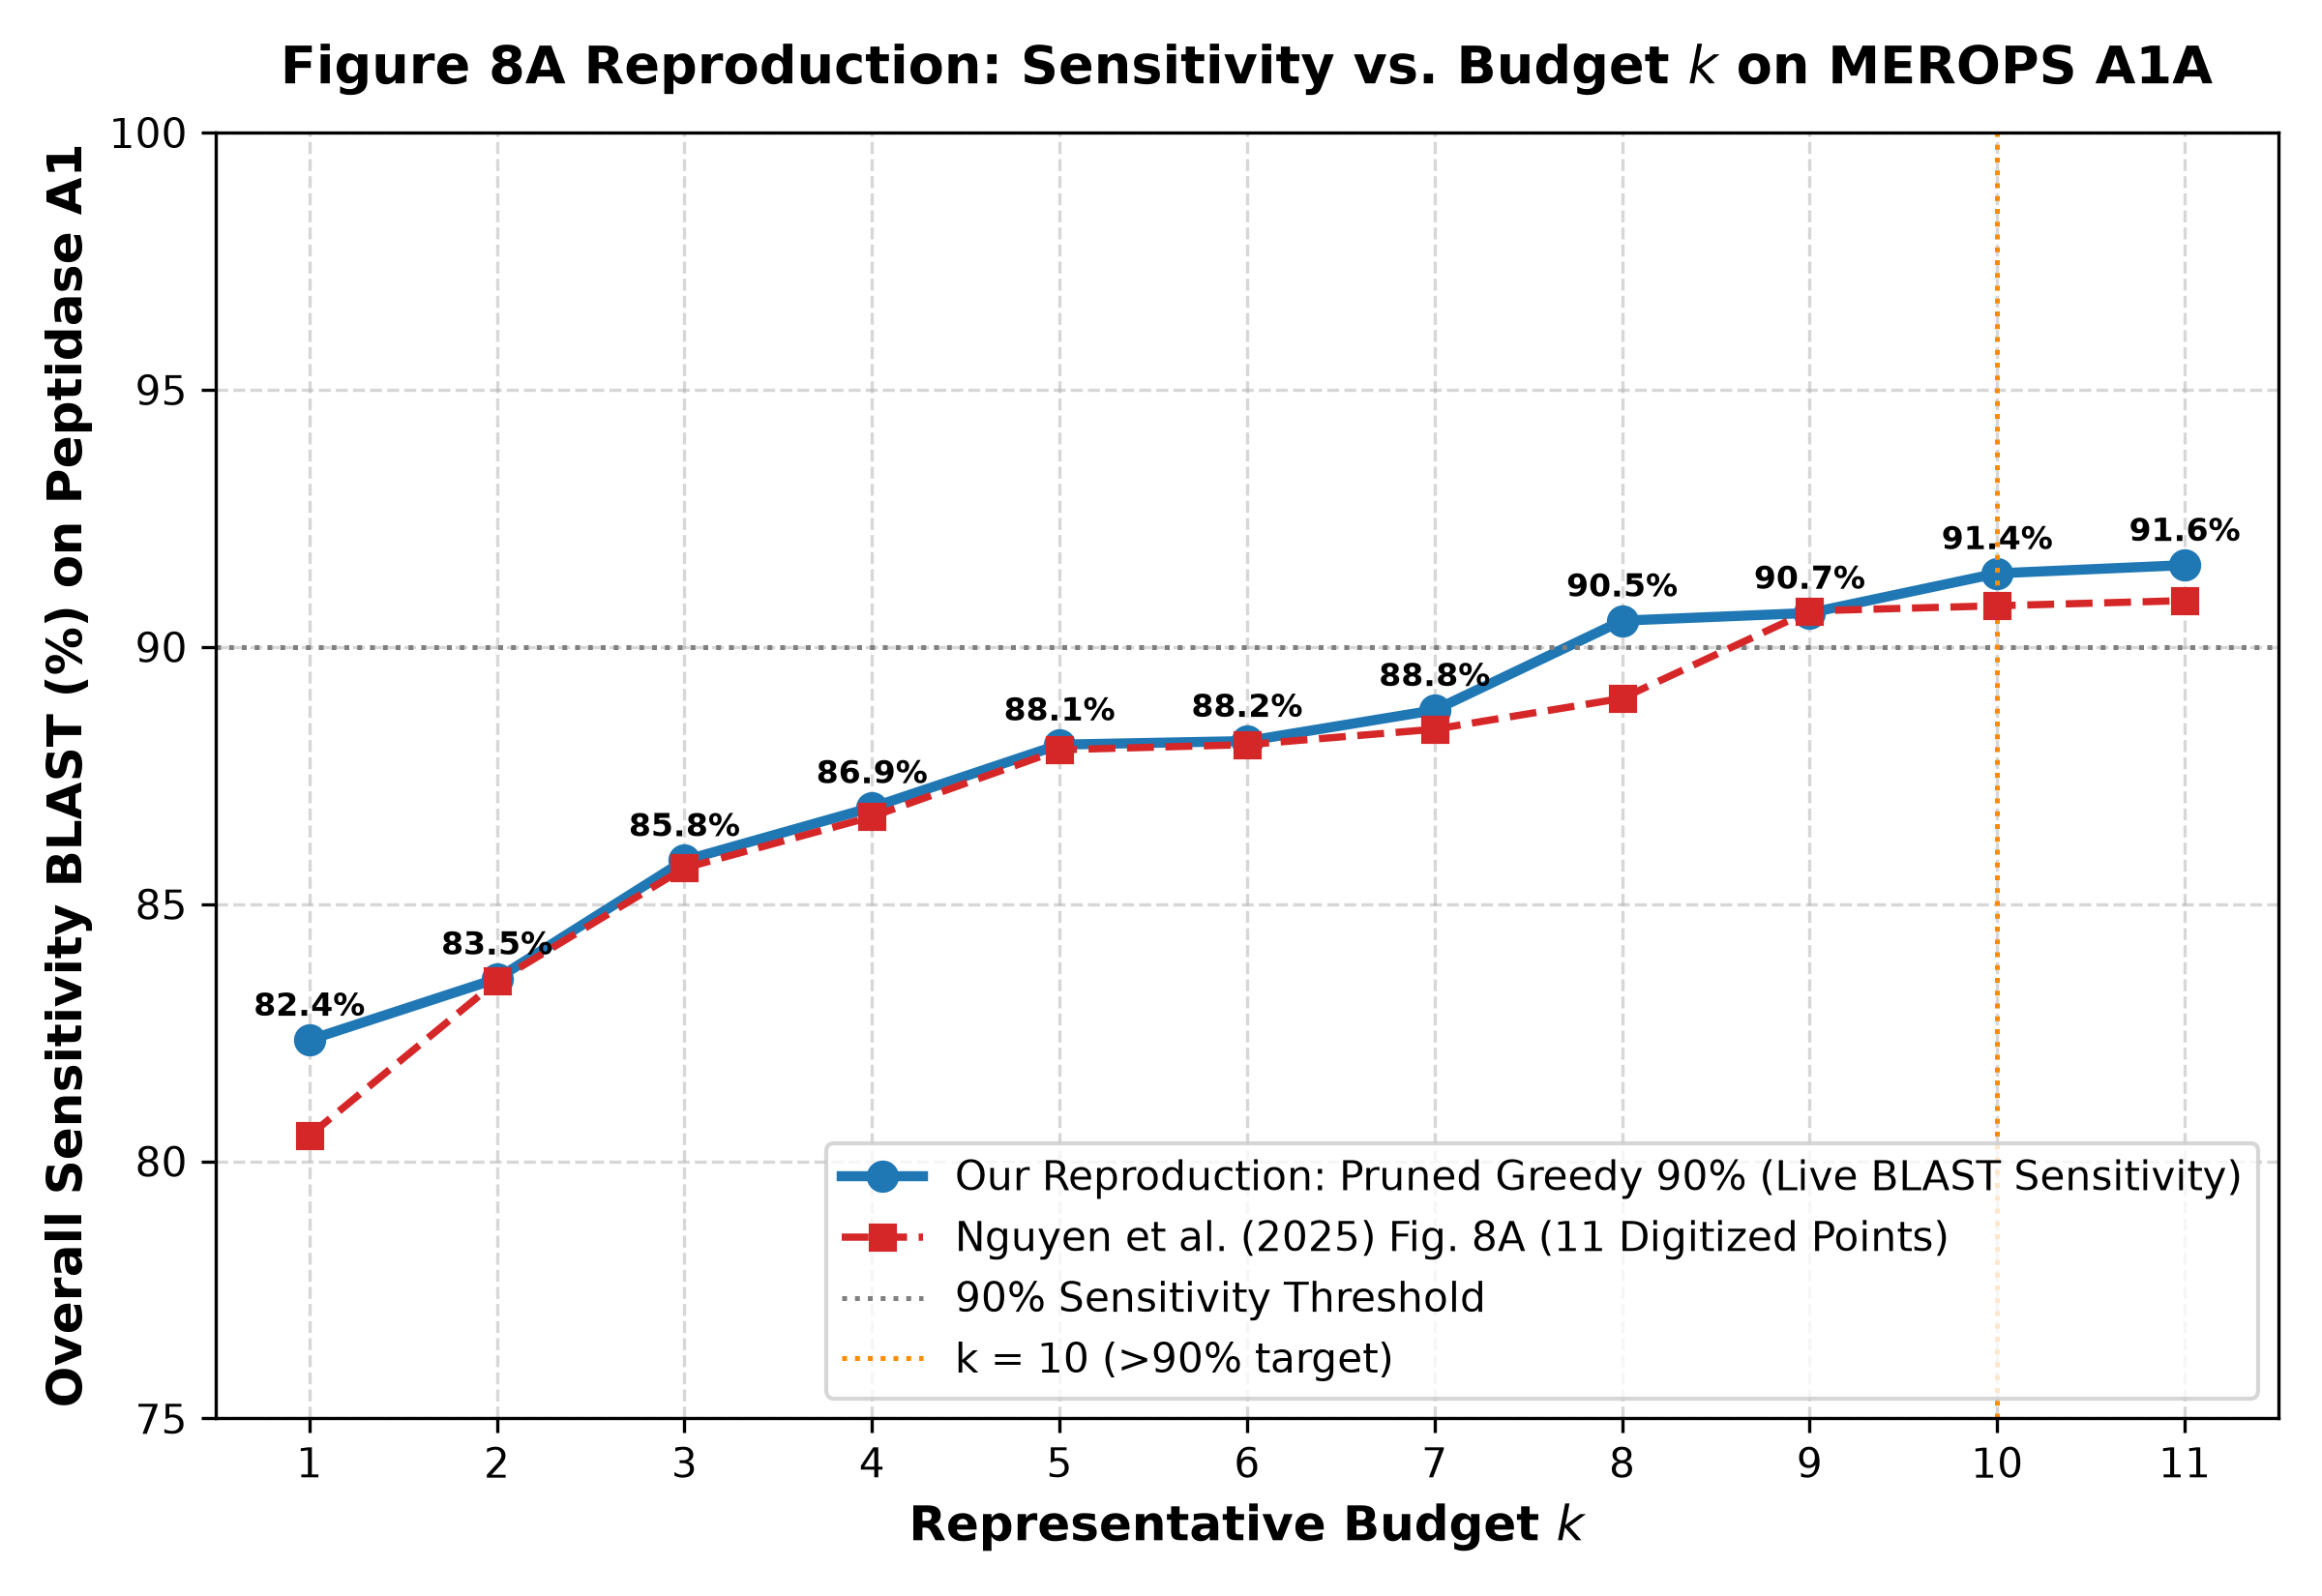
\includegraphics[width=0.84\textwidth]{Images/figures/exp1_a1a_sensitivity_vs_k.png}
    \caption{Đường cong Overall Sensitivity BLAST (\%) tái hiện trên Family Peptidase A1 đối chiếu với 11 điểm công bố tại hình 8A của Nguyen và cộng sự~\cite{nguyen2025}.}
    \label{fig:exp1_sensitivity}
\end{figure}

Số liệu tại bảng~\ref{tab:exp1_milestones} và hình~\ref{fig:exp1_sensitivity} khẳng định quy trình tái hiện thực nghiệm của đề tài đối chuẩn thành công công bố hình 8A của Nguyen và cộng sự~\cite{nguyen2025} với sai số tuyệt đối trung bình chỉ là $0{,}51\%$. Độ lệch giữa kết quả đo đạc thực nghiệm và dữ liệu công bố dao động trong biên độ hẹp từ $-0{,}04\%$ đến $+1{,}86\%$, tái hiện chuẩn xác xu thế tăng trưởng của chỉ số Overall Sensitivity khi vượt ngưỡng $90\%$ tại mốc ngân sách $k = 8$, đạt $90{,}51\%$ và nhận diện thành công $12.044$ trên $13.307$ chuỗi protein. Sự tương đồng định lượng này khẳng định thuật toán Pruned Greedy 90\% cùng ma trận tương đồng chuỗi $\mathbf{S}_{\text{BLAST}}$ đã tái lập chính xác mô hình cơ sở, tạo nền tảng vững chắc cho các thử nghiệm cải tiến tiếp theo.

Tuy nhiên, khi phân tích sâu cơ chế phân bổ ở cấp độ Subfamily, kết quả đối chứng làm sáng tỏ điểm mù phương pháp luận then chốt của mô hình không trọng số khi đánh giá toàn cục. Trong khi trên tập dữ liệu $13.307$ chuỗi thô, chỉ với một đại diện duy nhất ($k = 1$), chỉ số Overall Sensitivity đạt tới $82{,}36\%$ với $10.959$ chuỗi nhờ tích lũy bao phủ chéo sang các Subfamily khác và khối chuỗi chưa phân loại [A01.UPA], thì khi chuyển sang tập dữ liệu phân họ chính thức $V_{\text{curated}}$ gồm $4.120$ chuỗi với quy tắc đối soát nội phân họ Within-Subfamily, chỉ số Overall Sensitivity suy giảm mạnh: đại diện đầu tiên thuộc Subfamily lớn A01.001 chỉ thu hồi được $146 / 4.120$ chuỗi cùng Subfamily, tương ứng chỉ số Overall Sensitivity chỉ đạt $3{,}54\%$ và để lại $114$ trên $115$ Subfamily ở mức $0{,}0\%$ Sensitivity ($\text{Rare Sensitivity} = 0{,}0\%$, $\text{Macro-Average Sensitivity} = 0{,}87\%$). Tại mốc $k = 11$, chỉ số Overall Sensitivity nội phân họ của mô hình cơ sở không trọng số chỉ đạt $38{,}06\%$ với $1.568 / 4.120$ chuỗi và vẫn để sót $105$ trên $115$ Subfamily ở mức $0{,}0\%$. Kết quả thực nghiệm này làm rõ hạn chế cốt lõi của phương thức đánh giá toàn cục, chỉ ra rằng mức độ bao phủ trên $90\%$ ở bài báo gốc phần lớn được tạo thành từ hiện tượng bao phủ chéo ngoài ranh giới Subfamily.

\FloatBarrier
\phantomsection\label{sec:branch_2}
\phantomsection\label{subsec:branch2_mechanism}
\phantomsection\label{subsec:branch2_pareto}
\phantomsection\label{subsec:branch2_zero_cov}

Nhằm khắc phục điểm mù này, thử nghiệm 2 áp dụng nguyên tắc cô lập biến số: giữ nguyên không gian tương đồng chuỗi cơ sở NCBI BLASTp nhưng chuyển dịch sang tập dữ liệu phân họ chính thức $V_{\text{curated}}$ gồm $4.120$ chuỗi thuộc $115$ Subfamily, đồng thời đưa vào họ hàm mục tiêu có trọng số nghịch đảo quy mô Subfamily $w_v^{(\alpha)} = n_g^{-\alpha}$ với hệ số phạt quy mô nhóm $\alpha \in \{0{,}0, \, 0{,}5, \, 1{,}0\}$ đã định nghĩa tại công thức~\eqref{eq:sample_weight_formula}. Đồng thời, quy trình đo đạc áp dụng thống nhất cơ chế bao phủ nội phân họ Within-Subfamily Live BLASTp ở ngưỡng $E \le 10^{-7}$: chỉ các chuỗi đại diện thực sự thuộc về Subfamily $g$ mới được sử dụng làm chuỗi truy vấn đối soát với các thành viên của chính Subfamily đó, ngăn chặn nguy cơ sai lệch bao phủ chéo ngoài ranh giới phân họ.

Tại mốc ngân sách cơ sở $k = G = 115$, hàm mục tiêu có trọng số với $\alpha = 0{,}5$ đạt hiệu quả cao trên cả hai mục tiêu khi nâng chỉ số Rare Sensitivity tăng gấp $26{,}6$ lần, từ $2{,}22\%$ lên $59{,}11\%$, và chỉ số Macro-Average Sensitivity tăng thêm $+29{,}59\%$, từ $49{,}28\%$ lên $78{,}87\%$, trong khi chỉ số Overall Sensitivity không suy giảm mà tăng nhẹ từ $93{,}57\%$ lên $94{,}13\%$. Bảng~\ref{tab:exp2_milestones} tổng hợp kết quả tại các mốc ngân sách chiến lược.

\begin{table}[htbp!]
\centering
\caption{So sánh hiệu năng của ba chế độ trọng số $\alpha$ trên không gian tương đồng BLASTp tại các mốc ngân sách chiến lược theo cơ chế Within-Subfamily Live BLASTp.}
\label{tab:exp2_milestones}
\vspace{4pt}
\small
\resizebox{\textwidth}{!}{%
\begin{tabular}{ccrrrr}
\toprule
\textbf{Ngân sách $k$} & \textbf{Hệ số $\alpha$} & \textbf{Overall Sensitivity (\%)} & \textbf{Rare Sensitivity (\%)} & \textbf{Macro-Average Sensitivity (\%)} & \textbf{Zero-Sensitivity Count} \\
\midrule
$k = 15$  & 0{,}0 & 44{,}66 & 0{,}00  & 12{,}11 & 101 / 115 \\
          & 0{,}5 & 44{,}61 & 0{,}00  & 12{,}10 & 101 / 115 \\
          & 1{,}0 & 27{,}86 & 8{,}89  & 13{,}04 & 100 / 115 \\
\midrule
$k = 30$  & 0{,}0 & 71{,}65 & 0{,}00  & 23{,}87 & 87 / 115 \\
          & 0{,}5 & 62{,}72 & 4{,}44  & 25{,}15 & 86 / 115 \\
          & 1{,}0 & 48{,}16 & 26{,}67 & 26{,}03 & 85 / 115 \\
\midrule
$k = 60$  & 0{,}0 & 88{,}83 & 2{,}22  & 37{,}74 & 71 / 115 \\
          & 0{,}5 & 84{,}95 & 11{,}11 & 47{,}36 & 60 / 115 \\
          & 1{,}0 & 62{,}57 & 57{,}04 & 50{,}95 & 56 / 115 \\
\midrule
$k = 115$ & 0{,}0  & 93{,}57 & 2{,}22  & 49{,}28 & 58 / 115 \\
          & 0{,}5   & \textbf{94{,}13} & \textbf{59{,}11} & \textbf{78{,}87} & \textbf{23 / 115} \\
          & 1{,}0 & 79{,}08 & \textbf{91{,}11} & \textbf{83{,}44} & \textbf{18 / 115} \\
\bottomrule
\end{tabular}%
}
\end{table}

Số liệu tại bảng~\ref{tab:exp2_milestones} cho thấy sự cải thiện rõ nét khi áp dụng hàm mục tiêu có trọng số. Bên cạnh cấu hình trọng số cân bằng $\alpha = 0{,}5$, chế độ bình đẳng nhóm $\alpha = 1{,}0$ nâng chỉ số Rare Sensitivity lên mức cao nhất $91{,}11\%$, gấp $41{,}0$ lần so với mô hình cơ sở không trọng số, bảo tồn $41$ trên $45$ Subfamily hiếm nhưng chấp nhận sự đánh đổi khi chỉ số Overall Sensitivity giảm về $79{,}08\%$.

\begin{figure}[htbp!]
    \centering
    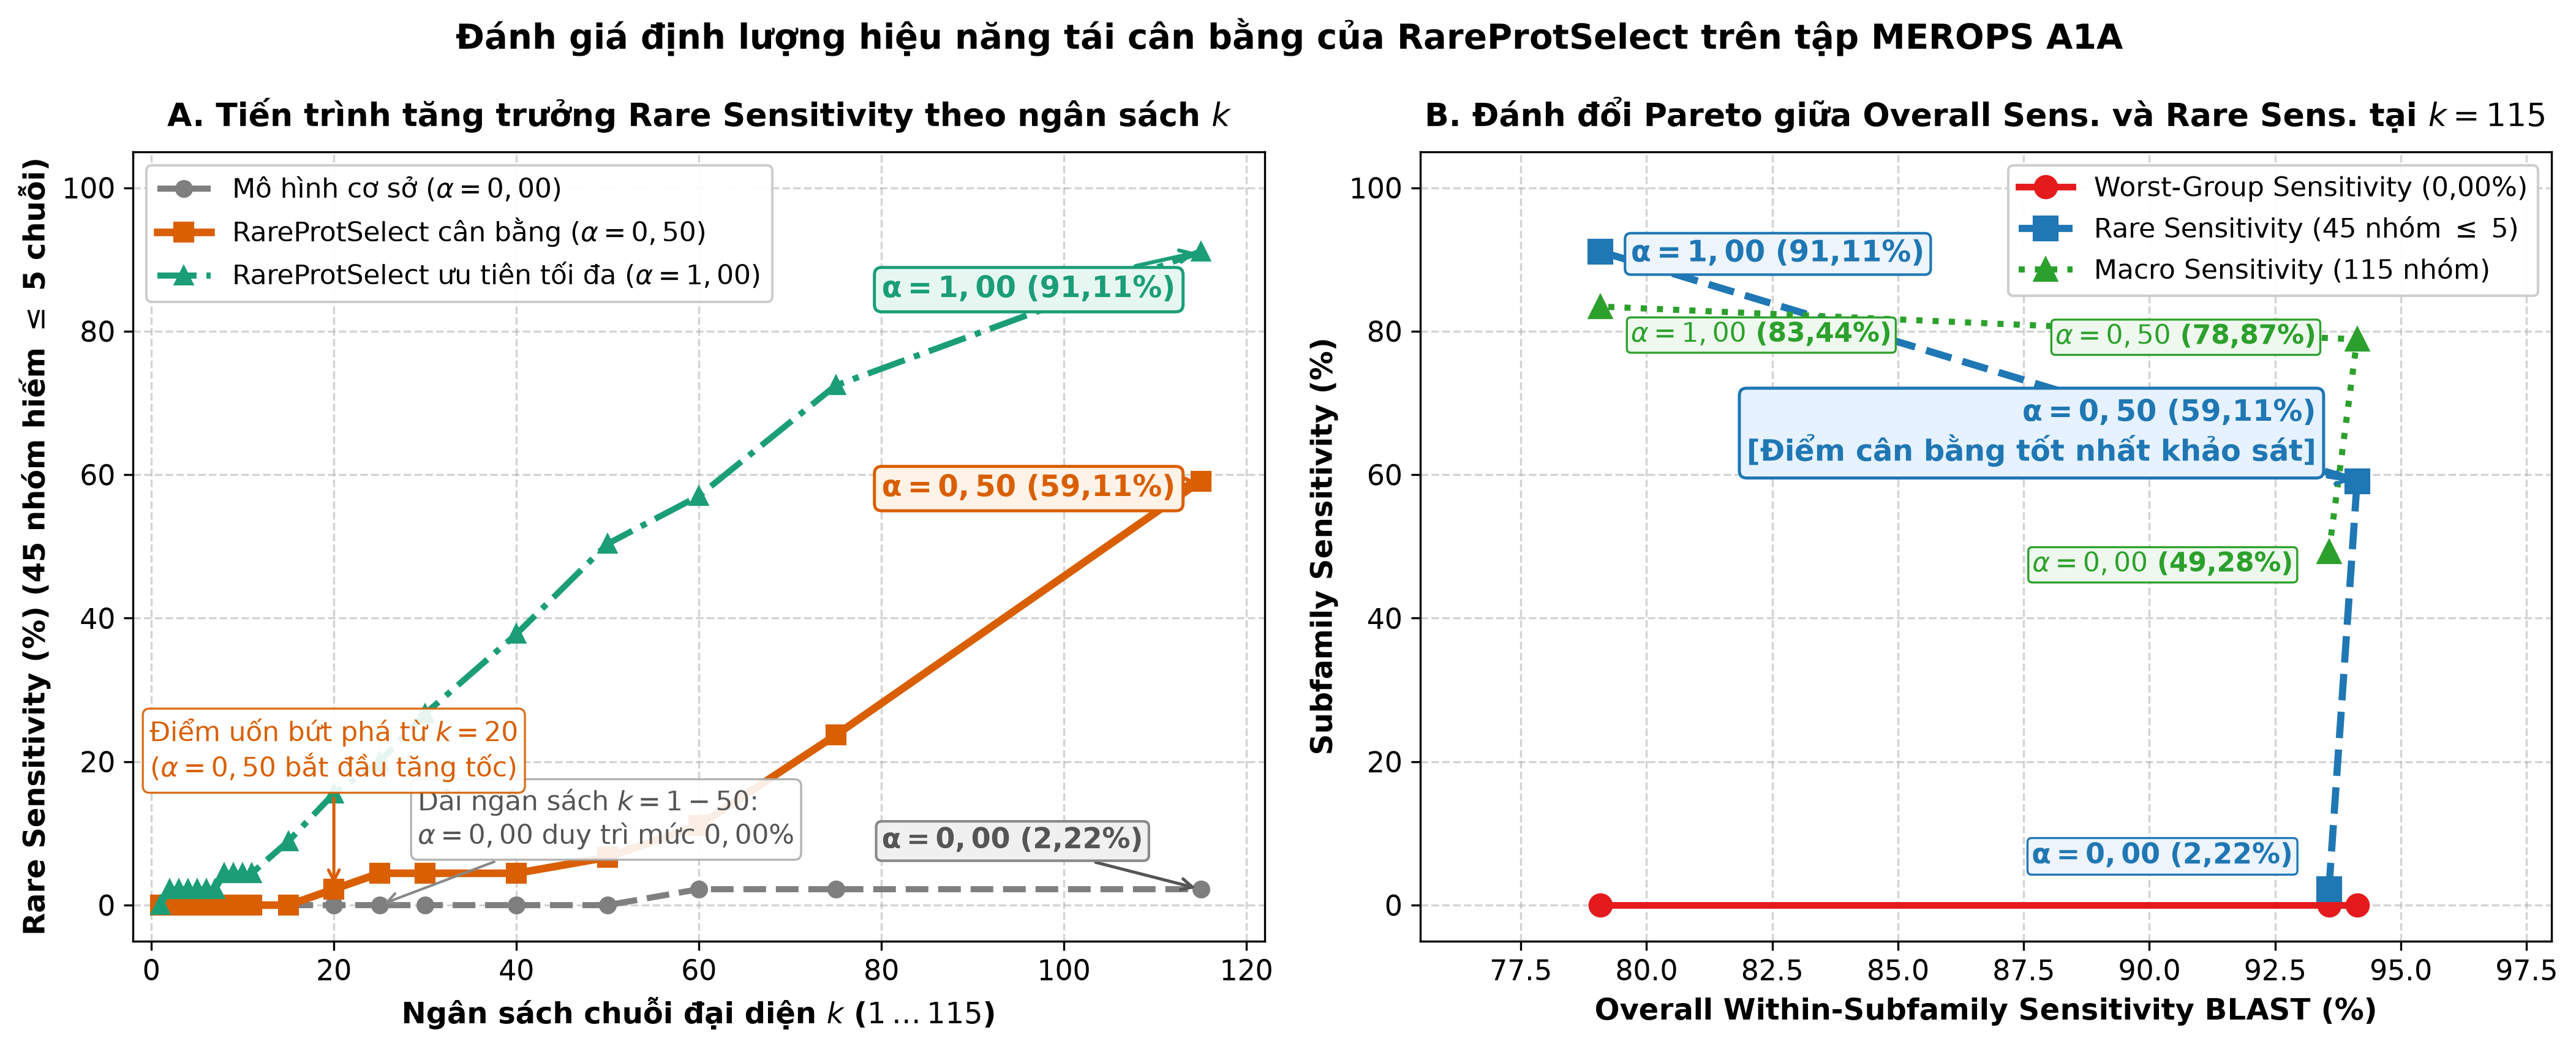
\includegraphics[width=0.92\textwidth]{Images/figures/exp2_pareto_tradeoff.png}
    \caption{Tương quan đánh đổi giữa chỉ số Overall Sensitivity và Rare Sensitivity tại hai mốc ngân sách $k = 11$ và $k = 115$ trên không gian tương đồng chuỗi BLASTp.}
    \label{fig:exp2_pareto}
\end{figure}

Mối quan hệ đánh đổi đa mục tiêu và xu hướng biến thiên của bốn chỉ số được minh họa tại hình~\ref{fig:exp2_pareto} và hình~\ref{fig:exp2_metrics}. Đồ thị làm rõ sự khác biệt giữa hai miền ngân sách: ở vùng ngân sách nhỏ $k = 11$ (hình~\ref{fig:exp2_pareto}A), sự đánh đổi đa mục tiêu thể hiện rõ khi $\alpha = 0{,}5$ có Overall Sensitivity đạt $32{,}60\%$ (thấp hơn $38{,}06\%$ của $\alpha = 0{,}0$) trong khi Rare Sensitivity vẫn bằng $0{,}0\%$ (chỉ có Macro-Average Sensitivity tăng nhẹ từ $8{,}68\%$ lên $9{,}56\%$); phải đến mốc ngân sách đủ lớn $k = G = 115$ (hình~\ref{fig:exp2_pareto}B), khi các Subfamily lớn đã đạt bão hòa nội nhóm, điểm biểu diễn của $\alpha = 0{,}5$ mới nằm ở góc trên bên phải so với $\alpha = 0{,}0$, nâng Rare Sensitivity lên $59{,}11\%$ mà không làm suy giảm Overall Sensitivity ($94{,}13\%$ so với $93{,}57\%$), trong khi $\alpha = 1{,}0$ tại $k = 115$ vẫn đánh đổi giảm $14{,}49$ điểm phần trăm Overall Sensitivity ($79{,}08\%$). Đồ thị hình~\ref{fig:exp2_metrics} thể hiện rõ sự chênh lệch giữa các chế độ trọng số: đường Rare Sensitivity của $\alpha = 0{,}0$ duy trì ở mức $0{,}0\%$ trong toàn bộ khoảng từ $k = 1$ đến $k = 50$, trong khi đường $\alpha = 1{,}0$ tăng trưởng nhanh ngay từ mốc $k = 2$ đạt $2{,}22\%$ và đạt $50{,}37\%$ tại mốc ngân sách $k = 50$. Đường Worst-Group Sensitivity (hình~\ref{fig:exp2_metrics}B) duy trì bằng $0{,}0\%$ xuyên suốt $k \in [1..115]$ do tại mọi mốc này vẫn còn ít nhất 18 Subfamily chưa có đại diện.

\begin{figure}[htbp!]
    \centering
    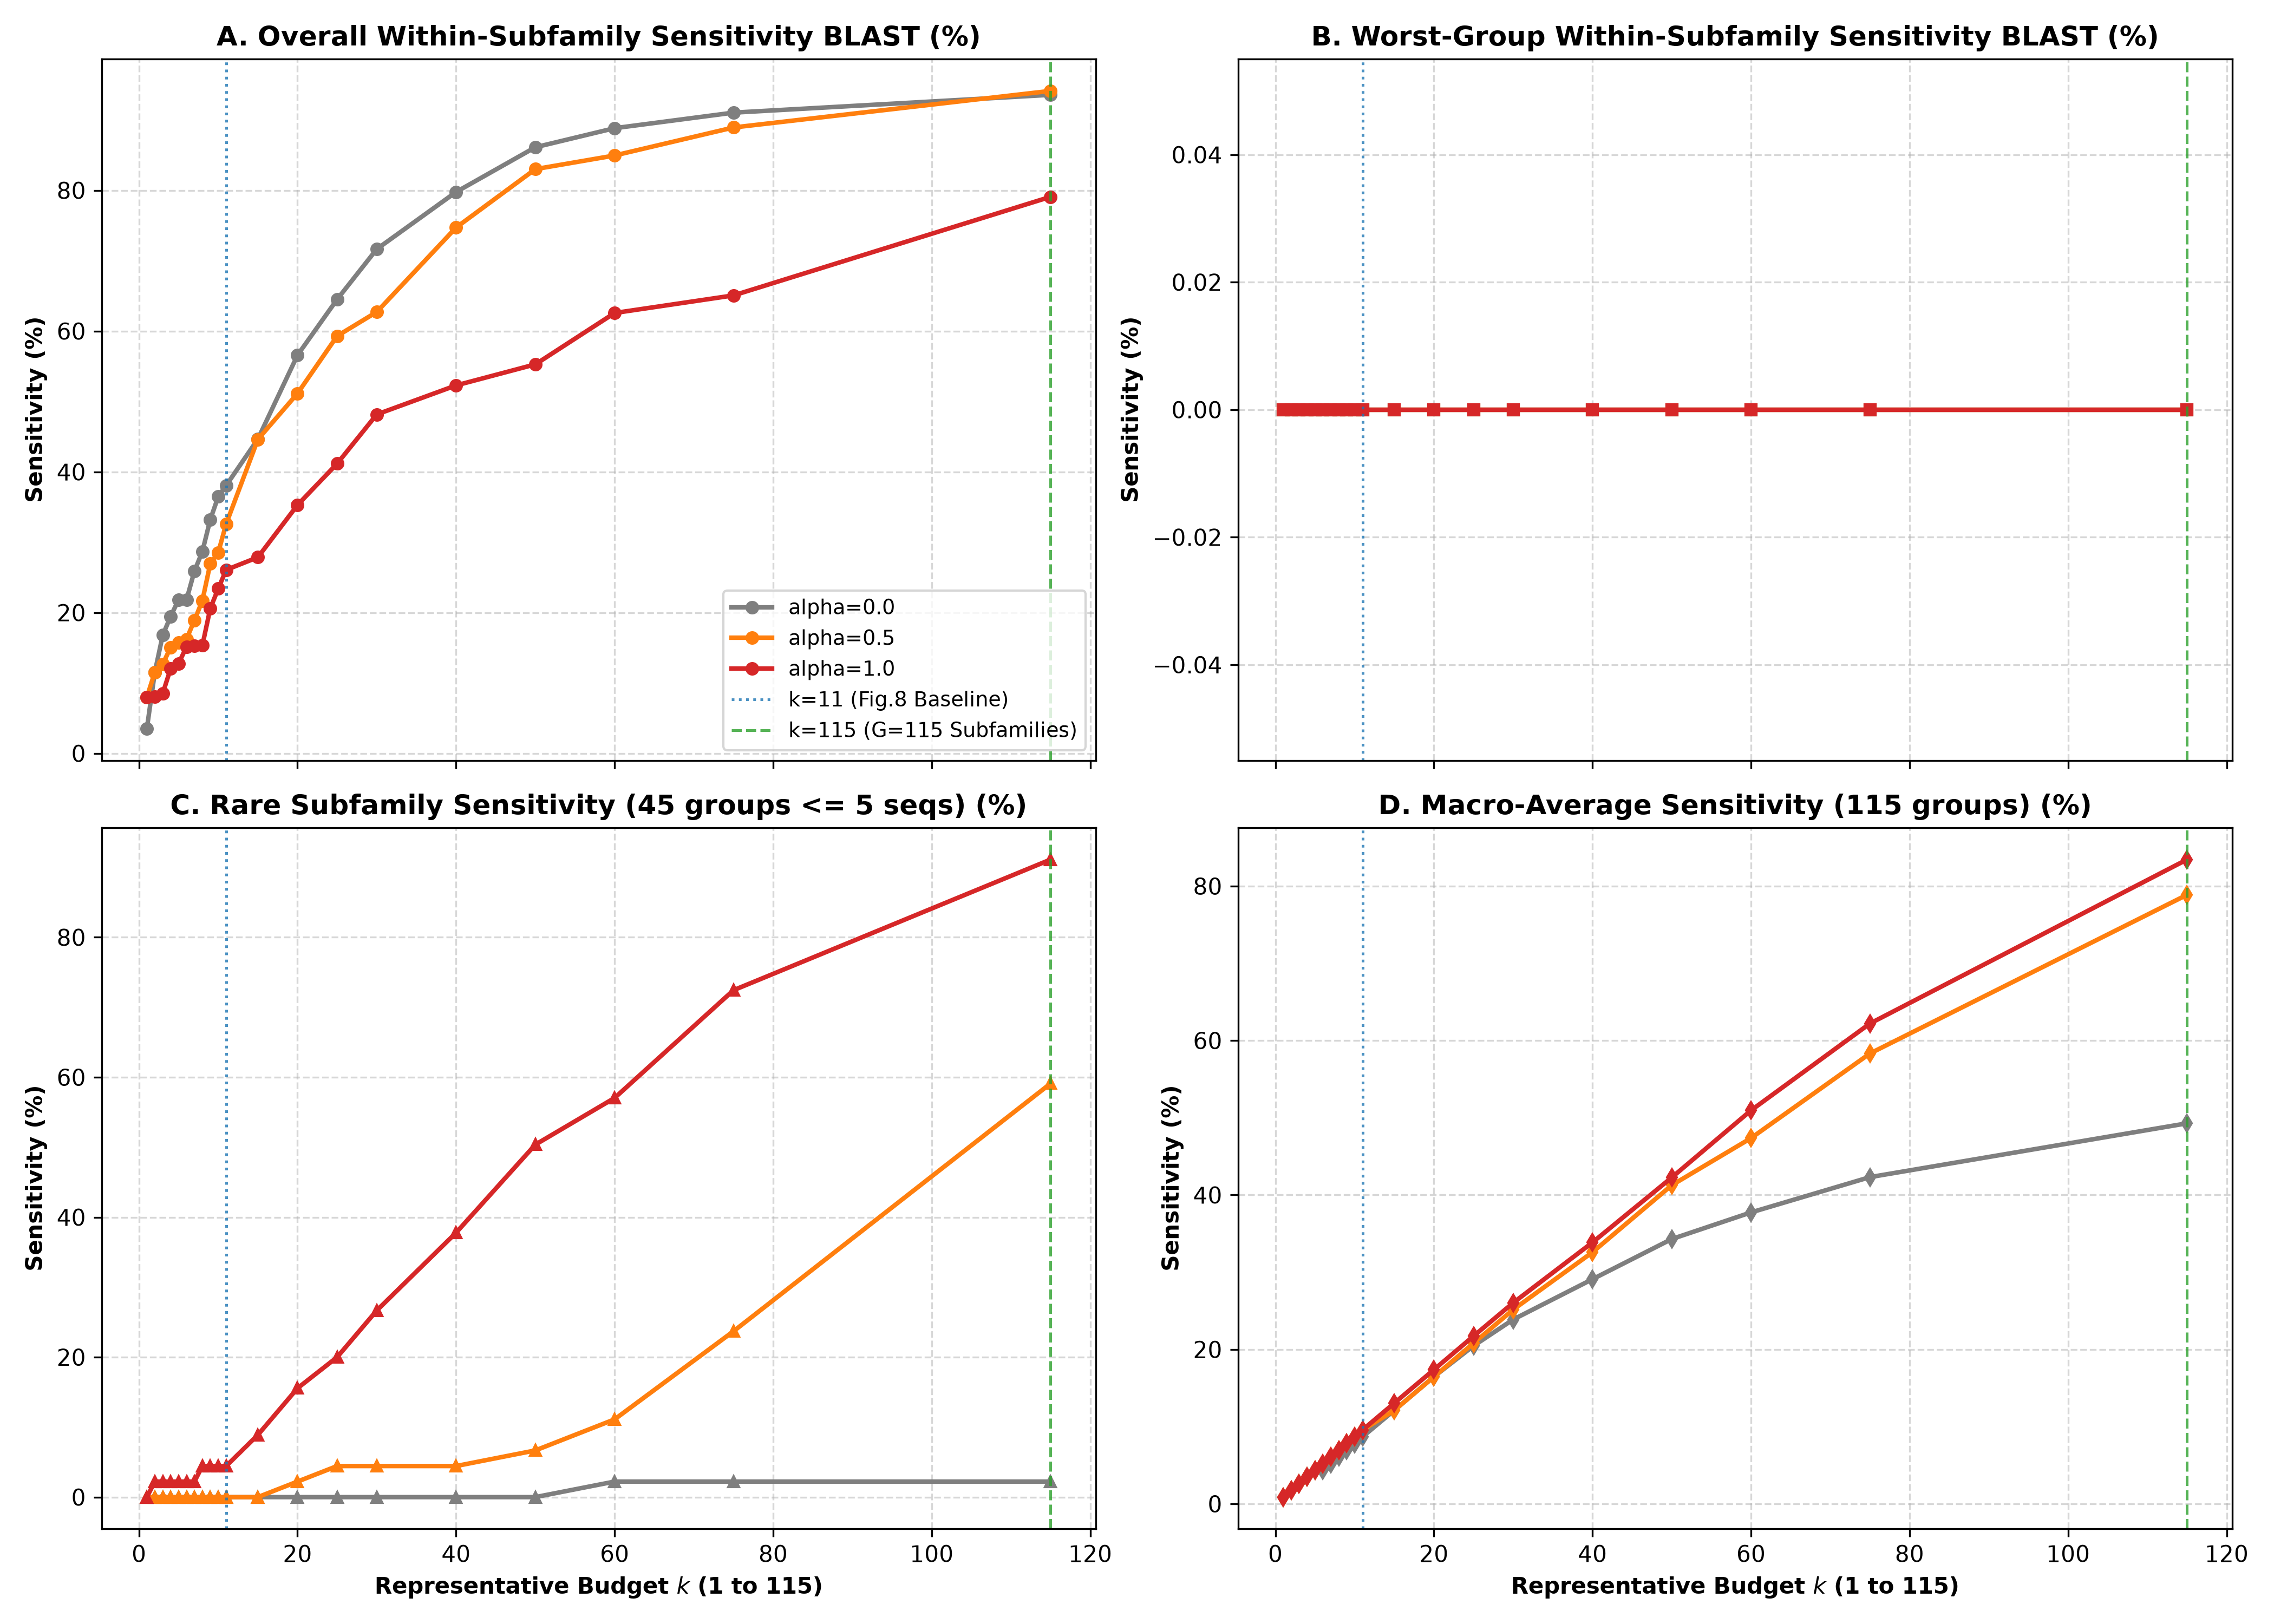
\includegraphics[width=0.92\textwidth]{Images/figures/exp2_metrics_vs_k.png}
    \caption{Đường cong biến thiên của bốn thước đo Sensitivity nội phân họ theo ngân sách $k \in [1..115]$ qua ba chế độ trọng số $\alpha \in \{0{,}0, \, 0{,}5, \, 1{,}0\}$ trên không gian BLASTp.}
    \label{fig:exp2_metrics}
\end{figure}

Thiết lập trọng số $\alpha = 0{,}5$ khôi phục tính đại diện cho $35$ Subfamily, kéo giảm số lượng phân họ có chỉ số Sensitivity bằng 0 từ $58$ xuống còn $23$ Subfamily tại mốc ngân sách $k = 115$. Hình~\ref{fig:exp2_zero_cov} lượng hóa số lượng phân họ có chỉ số Sensitivity bằng 0 theo hệ số $\alpha$, cho thấy phương pháp không trọng số của bài báo gốc để sót tới $58$ trên tổng số $115$ Subfamily, chiếm $50{,}43\%$, ở mức $0{,}0\%$ Sensitivity. Chế độ $\alpha = 1{,}0$ tiếp tục thu hẹp con số này về mức $18$ Subfamily. Kết quả này khẳng định hiệu quả của mô hình đề xuất: hàm mục tiêu có trọng số với $\alpha = 0{,}5$ khôi phục đáng kể tính đại diện cho các phân họ hiếm trên không gian BLASTp mà không làm giảm chỉ số Overall Sensitivity, nhờ cơ chế hạn chế các lượt chọn dư thừa ở các nhóm lớn.

\begin{figure}[htbp!]
    \centering
    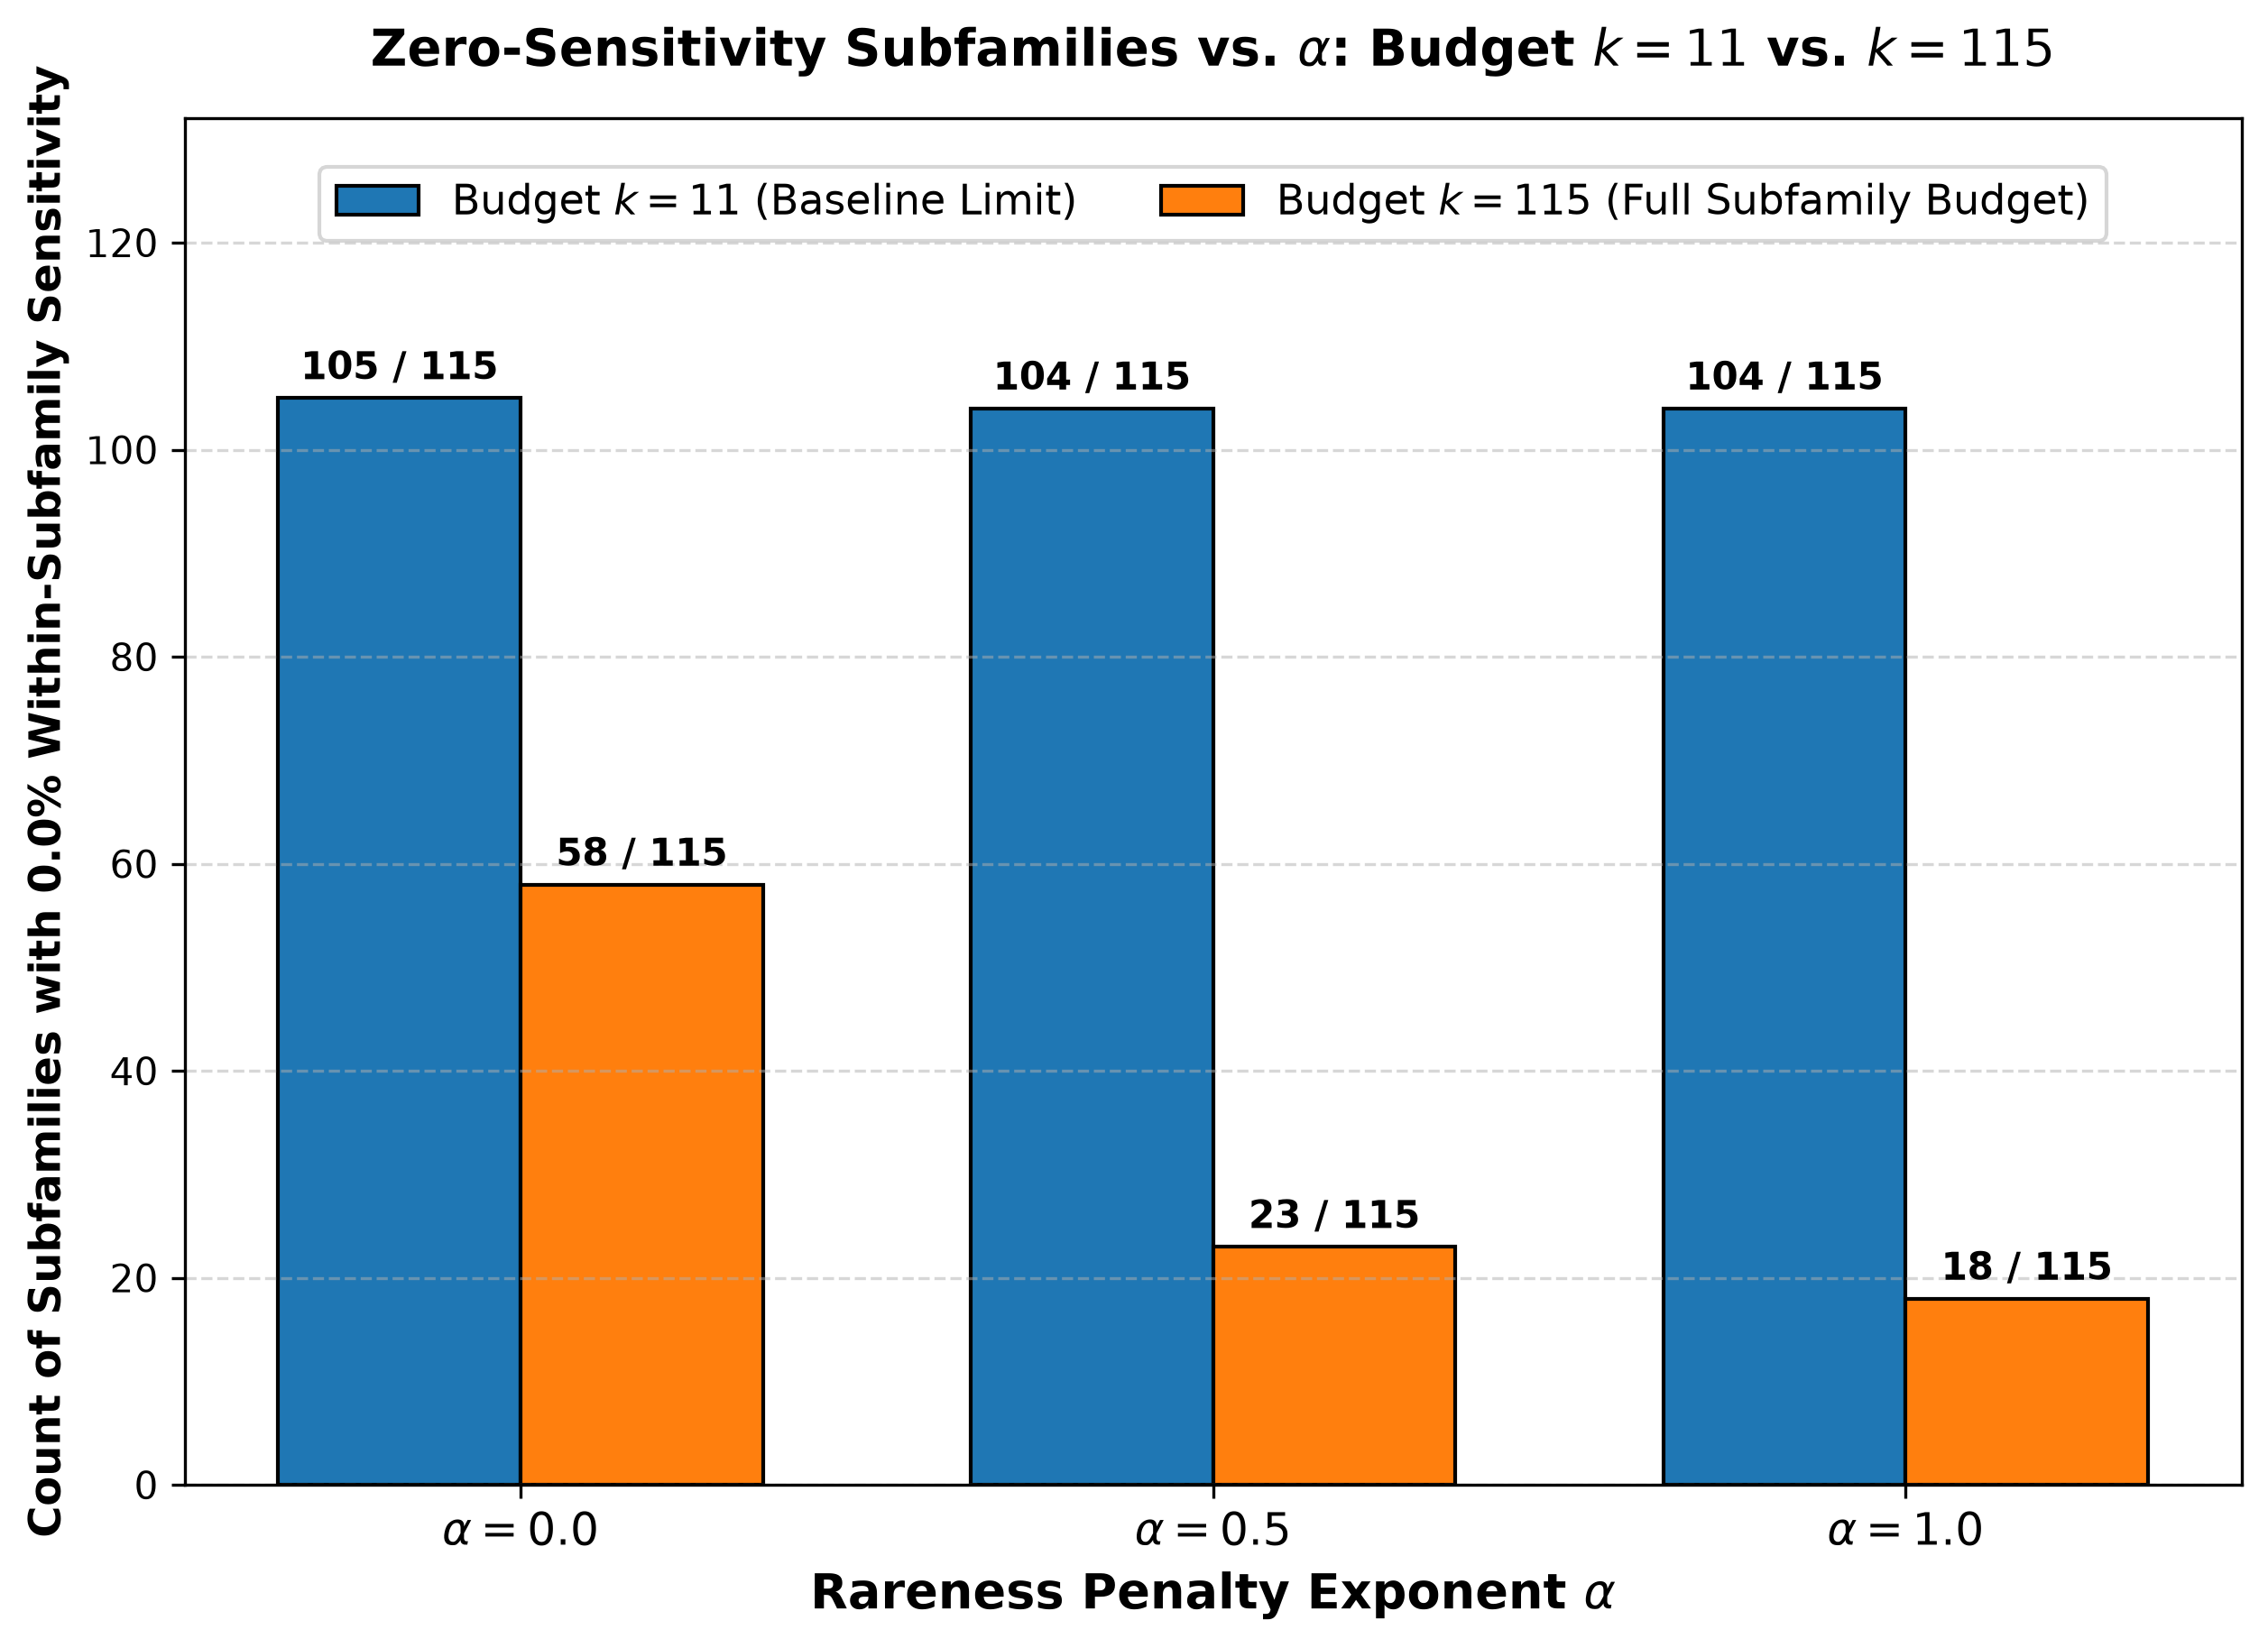
\includegraphics[width=0.82\textwidth]{Images/figures/exp2_zero_cov_vs_alpha.png}
    \caption{Biến thiên chỉ số Zero-Sensitivity Count theo hệ số $\alpha$ tại hai mốc ngân sách $k = 11$ và $k = 115$ trên không gian BLASTp.}
    \label{fig:exp2_zero_cov}
\end{figure}

\FloatBarrier\section{Khảo sát không gian ESM-2 và kiểm chứng chéo hai chiều}
\label{sec:esm_cross_evaluation}
\phantomsection\label{sec:branch_3}
\phantomsection\label{subsec:branch3_anisotropy}
\phantomsection\label{subsec:branch3_results}

Bên cạnh không gian tương đồng chuỗi rời rạc, hiệu năng bảo tồn đa dạng sinh học được khảo sát mở rộng trên không gian hình học liên tục ESM-2, kết hợp ma trận kiểm chứng chéo hai chiều nhằm đánh giá khả năng chuyển giao giữa hai hệ quy chiếu.

Tại thử nghiệm 3, giải thuật tối ưu hóa được thực thi trực tiếp trên ma trận tương đồng ngữ nghĩa $\mathbf{S}_{\text{ESM}}^{(\beta=0{,}70)}$ đã qua xử lý dịch tâm tại mục~\ref{subsec:mean_centering_technique} và đánh giá khả năng bao phủ cụm ngữ nghĩa bằng bốn thước đo hình học Within-Subfamily Coverage ESM. Trong không gian ngữ nghĩa liên tục, hàm mục tiêu có trọng số với $\alpha = 0{,}5$ nâng chỉ số Rare Coverage ESM tăng gấp $3{,}4$ lần, từ $12{,}85\%$ lên $43{,}21\%$, và chỉ số Macro-Average Coverage ESM tăng $+15{,}12\%$, từ $47{,}24\%$ lên $62{,}36\%$ tại ngân sách $k = 115$, trong khi chỉ số Overall Coverage ESM chỉ suy giảm nhẹ $-1{,}40\%$, từ $84{,}20\%$ xuống $82{,}80\%$. Bảng~\ref{tab:exp3_milestones} tổng hợp kết quả đo đạc qua ba chế độ trọng số tại các mốc ngân sách chiến lược.

\begin{table}[htbp!]
\centering
\caption{Hiệu năng bao phủ ngữ nghĩa nội phân họ Within-Subfamily Coverage ESM (\%) qua ba chế độ trọng số $\alpha$ tại các mốc ngân sách chiến lược.}
\label{tab:exp3_milestones}
\vspace{4pt}
\small
\resizebox{0.95\textwidth}{!}{%
\begin{tabular}{ccrrr}
\toprule
\textbf{Ngân sách $k$} & \textbf{Hệ số $\alpha$} & \textbf{Overall Coverage ESM (\%)} & \textbf{Rare Coverage ESM (\%)} & \textbf{Macro-Average Coverage ESM (\%)} \\
\midrule
$k = 8$   & 0{,}0 & 18{,}34 & 0{,}00  & 6{,}38 \\
          & 0{,}5 & 14{,}22 & \textbf{2{,}22}  & 6{,}37 \\
          & 1{,}0 & 14{,}42 & \textbf{2{,}22}  & 6{,}37 \\
\midrule
$k = 30$  & 0{,}0 & 59{,}73 & 2{,}05  & 22{,}94 \\
          & 0{,}5 & 52{,}75 & \textbf{10{,}86} & 23{,}32 \\
          & 1{,}0 & 31{,}78 & \textbf{28{,}26} & 23{,}69 \\
\midrule
$k = 60$  & 0{,}0 & 73{,}78 & 6{,}40  & 34{,}43 \\
          & 0{,}5 & 64{,}37 & \textbf{28{,}17} & 43{,}15 \\
          & 1{,}0 & 60{,}03 & \textbf{40{,}01} & 45{,}63 \\
\midrule
$k = 115$ & 0{,}0 & 84{,}20 & 12{,}85 & 47{,}24 \\
          & 0{,}5  & 82{,}80 & \textbf{43{,}21} & \textbf{62{,}36} \\
          & 1{,}0& 82{,}38 & \textbf{40{,}86} & 59{,}85 \\
\bottomrule
\end{tabular}%
}
\end{table}

Số liệu tại bảng~\ref{tab:exp3_milestones} cùng các đồ thị hình~\ref{fig:exp3_pareto} và hình~\ref{fig:exp3_metrics} khẳng định tính tổng quát của họ hàm mục tiêu có trọng số trong không gian hình học liên tục. Cần lưu ý rằng tại ngân sách nhỏ $k = 8$, ESM-2 ($\alpha = 0{,}5$) mới chọn được đúng $1 / 45$ Subfamily hiếm ($2{,}22\%$) và duy trì tỷ lệ này đến $k = 20$; trong khi trên không gian BLASTp, cấu hình $\alpha = 1{,}0$ đã chọn nhóm hiếm ngay từ $k = 2$ ($2{,}22\%$) và đạt $4{,}44\%$ tại $k = 8$. Lợi thế của ESM-2 ($\alpha = 0{,}5$) so với BLASTp ($\alpha = 0{,}5$) thể hiện rõ nhất ở dải ngân sách trung bình $k \in [25..60]$.

\begin{figure}[htbp!]
    \centering
    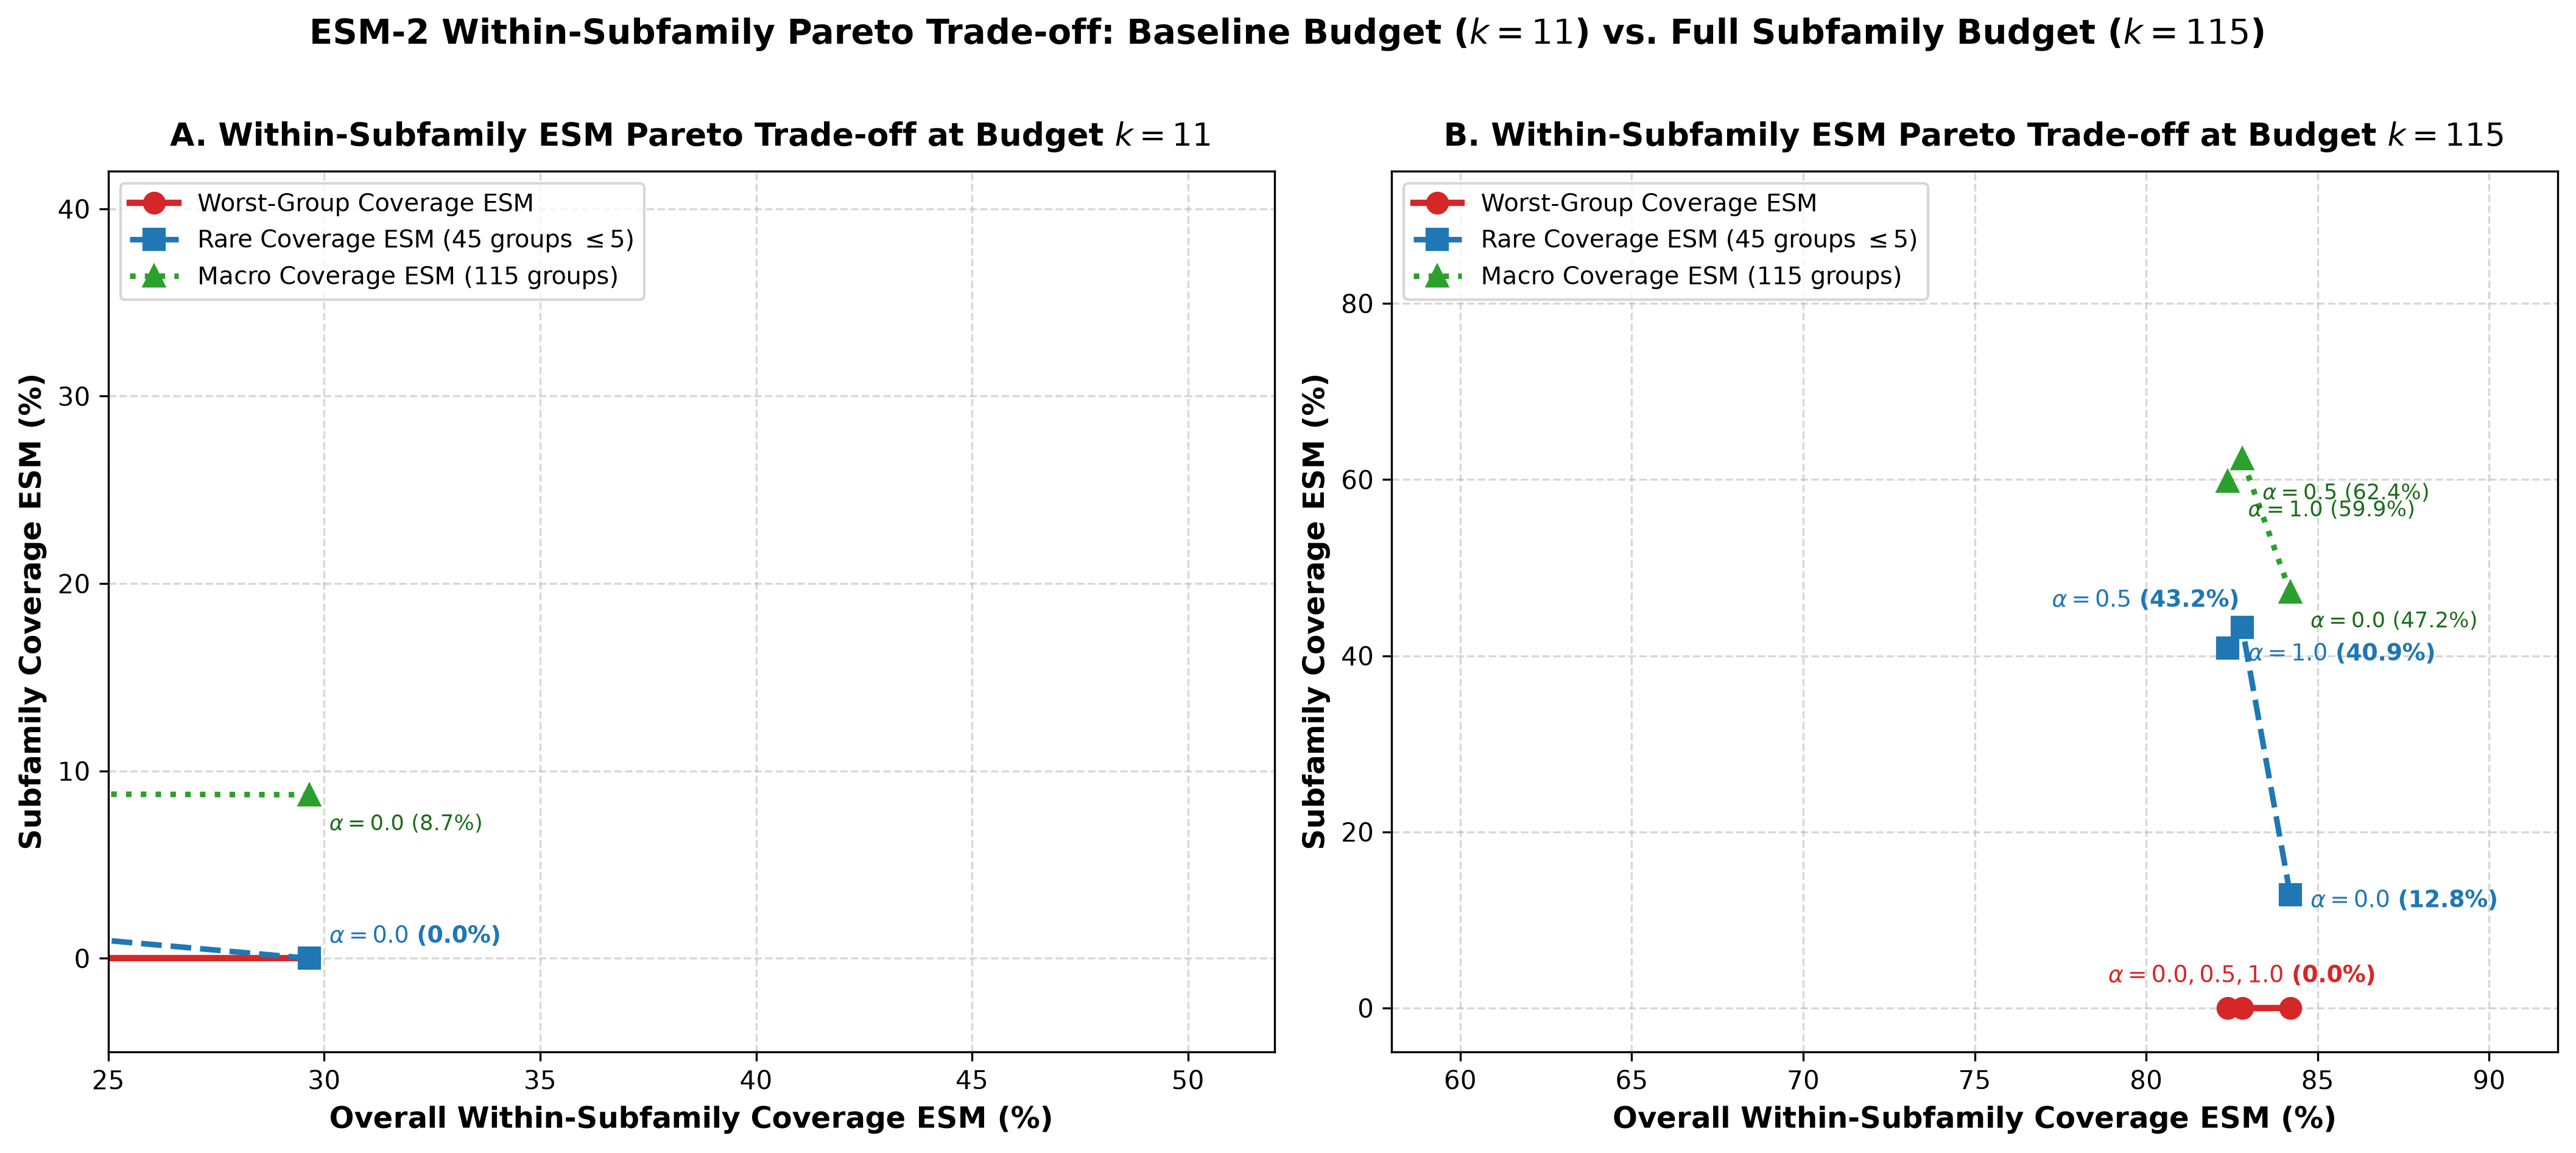
\includegraphics[width=0.92\textwidth]{Images/figures/exp3_pareto_tradeoff.png}
    \caption{Tương quan đánh đổi giữa Overall Coverage ESM và Rare Coverage ESM tại hai mốc ngân sách $k = 11$ và $k = 115$ trên không gian ngữ nghĩa ESM-2.}
    \label{fig:exp3_pareto}
\end{figure}

\begin{figure}[htbp!]
    \centering
    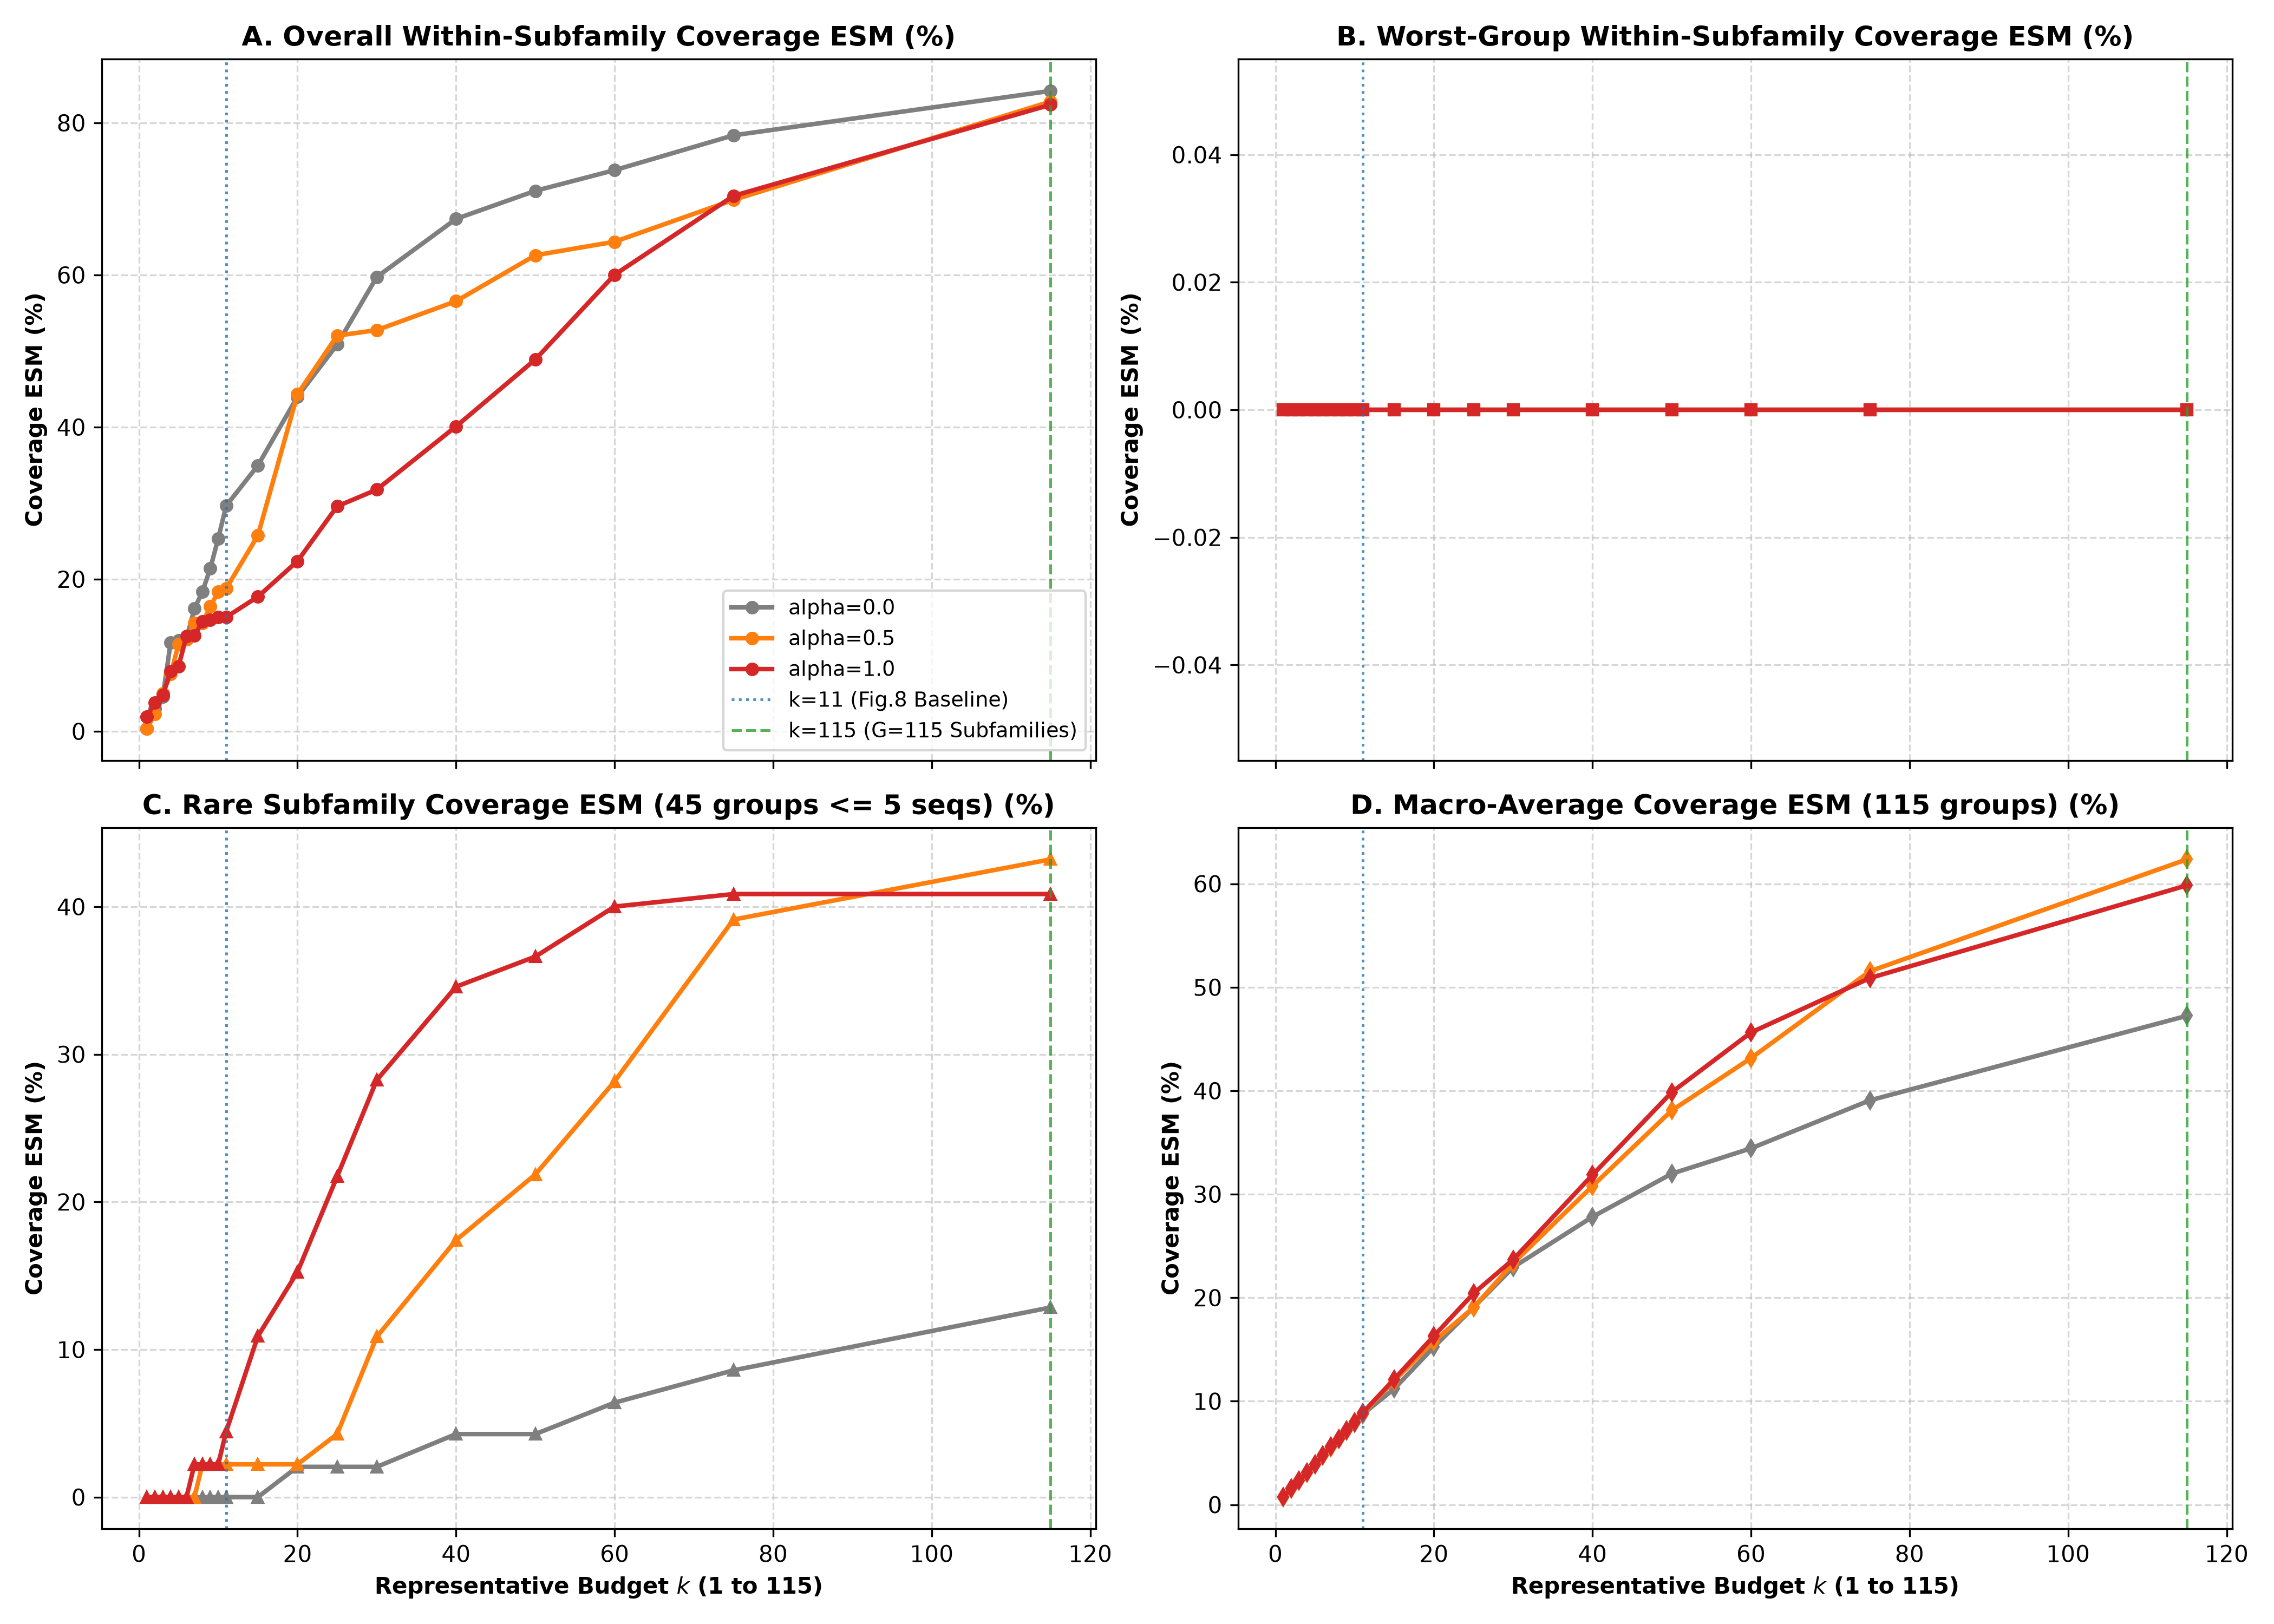
\includegraphics[width=0.92\textwidth]{Images/figures/exp3_metrics_vs_k.png}
    \caption{Đường cong biến thiên của bốn chỉ số Within-Subfamily Coverage ESM (\%) theo ngân sách $k \in [1..115]$ qua ba chế độ trọng số $\alpha$ trên không gian ESM-2.}
    \label{fig:exp3_metrics}
\end{figure}

\FloatBarrier
\phantomsection\label{sec:branch_4}
\phantomsection\label{subsec:branch4_matrix_design}
\phantomsection\label{subsec:branch4_crossover}
\phantomsection\label{subsec:branch4_math_explanation}

Nhằm kiểm soát hiện tượng thiên lệch khi đánh giá nội không gian, thử nghiệm 4 triển khai ma trận kiểm chứng chéo hai chiều $2 \times 2$ trên toàn bộ $120$ cấu hình thực nghiệm đối với cả hai hệ quy chiếu: thước đo sinh học thực nghiệm Within-Subfamily Live BLASTp ở ngưỡng $E \le 10^{-7}$ và thước đo hình học bổ trợ Within-Subfamily Coverage ESM trên ma trận $\mathbf{S}_{\text{ESM}}^{(\beta=0{,}70)}$. Toàn bộ $60$ cấu hình đường chéo chính khớp $100{,}00\%$ khi đối chiếu với kết quả gốc của thử nghiệm 2 và thử nghiệm 3.

Kiểm tra chéo hai chiều cho thấy sự đảo chiều về hiệu năng giữa hai không gian khi tăng ngân sách $k$: ở dải ngân sách nhỏ và vừa từ $k = 8$ đến $k = 75$, tập đại diện chọn bởi ESM-2 đạt kết quả cao hơn so với BLASTp, gấp từ $1{,}6$ lần đến $4{,}0$ lần; tuy nhiên, khi ngân sách tăng lên $k = 115$, tập đại diện chọn bởi BLASTp lại đạt kết quả cao hơn trên cả hai hệ quy chiếu đo đạc. Bảng~\ref{tab:exp4_cross_milestones} tổng hợp kết quả đối sánh hai chiều tại các mốc ngân sách khảo sát.

\begin{table}[htbp!]
\centering
\caption{Đối chiếu kiểm tra chéo hai chiều giữa đại diện chọn bởi BLASTp và đại diện chọn bởi ESM-2 trên cả hai hệ quy chiếu đo đạc tại các mốc ngân sách khảo sát.}
\label{tab:exp4_cross_milestones}
\vspace{4pt}
\small
\resizebox{\textwidth}{!}{%
\begin{tabular}{cccrrrr}
\toprule
\textbf{Không gian chọn} & \textbf{Hệ số $\alpha$} & \textbf{Ngân sách $k$} & \textbf{Overall Sensitivity (\%)} & \textbf{Rare Sensitivity (\%)} & \textbf{Overall Coverage ESM (\%)} & \textbf{Rare Coverage ESM (\%)} \\
\midrule
BLASTp & 0{,}0 & $k = 115$ & 93{,}57 & 2{,}22  & 87{,}47 & 2{,}05 \\
ESM-2  & 0{,}0 & $k = 115$ & 90{,}70 & \textbf{13{,}33} & 84{,}20 & \textbf{12{,}85} \\
\midrule
BLASTp & 0{,}5 & $k = 40$  & 74{,}71 & 4{,}44  & 68{,}71 & 4{,}27 \\
ESM-2  & 0{,}5 & $k = 40$  & 59{,}85 & \textbf{17{,}78} & 56{,}55 & \textbf{17{,}41} \\
\midrule
BLASTp & 0{,}5 & $k = 60$  & 84{,}95 & 11{,}11 & 77{,}91 & 10{,}83 \\
ESM-2  & 0{,}5 & $k = 60$  & 67{,}91 & \textbf{28{,}89} & 64{,}37 & \textbf{28{,}17} \\
\midrule
BLASTp & 0{,}5 & $k = 115$ & \textbf{94{,}13} & \textbf{59{,}11} & \textbf{86{,}88} & \textbf{58{,}29} \\
ESM-2  & 0{,}5 & $k = 115$ & 89{,}98 & 43{,}11 & 82{,}80 & 43{,}21 \\
\midrule
BLASTp & 1{,}0 & $k = 115$ & 79{,}08 & \textbf{91{,}11} & 72{,}75 & \textbf{89{,}69} \\
ESM-2  & 1{,}0 & $k = 115$ & 87{,}79 & 41{,}33 & 82{,}38 & 40{,}86 \\
\bottomrule
\end{tabular}%
}
\end{table}

\begin{figure}[htbp!]
    \centering
    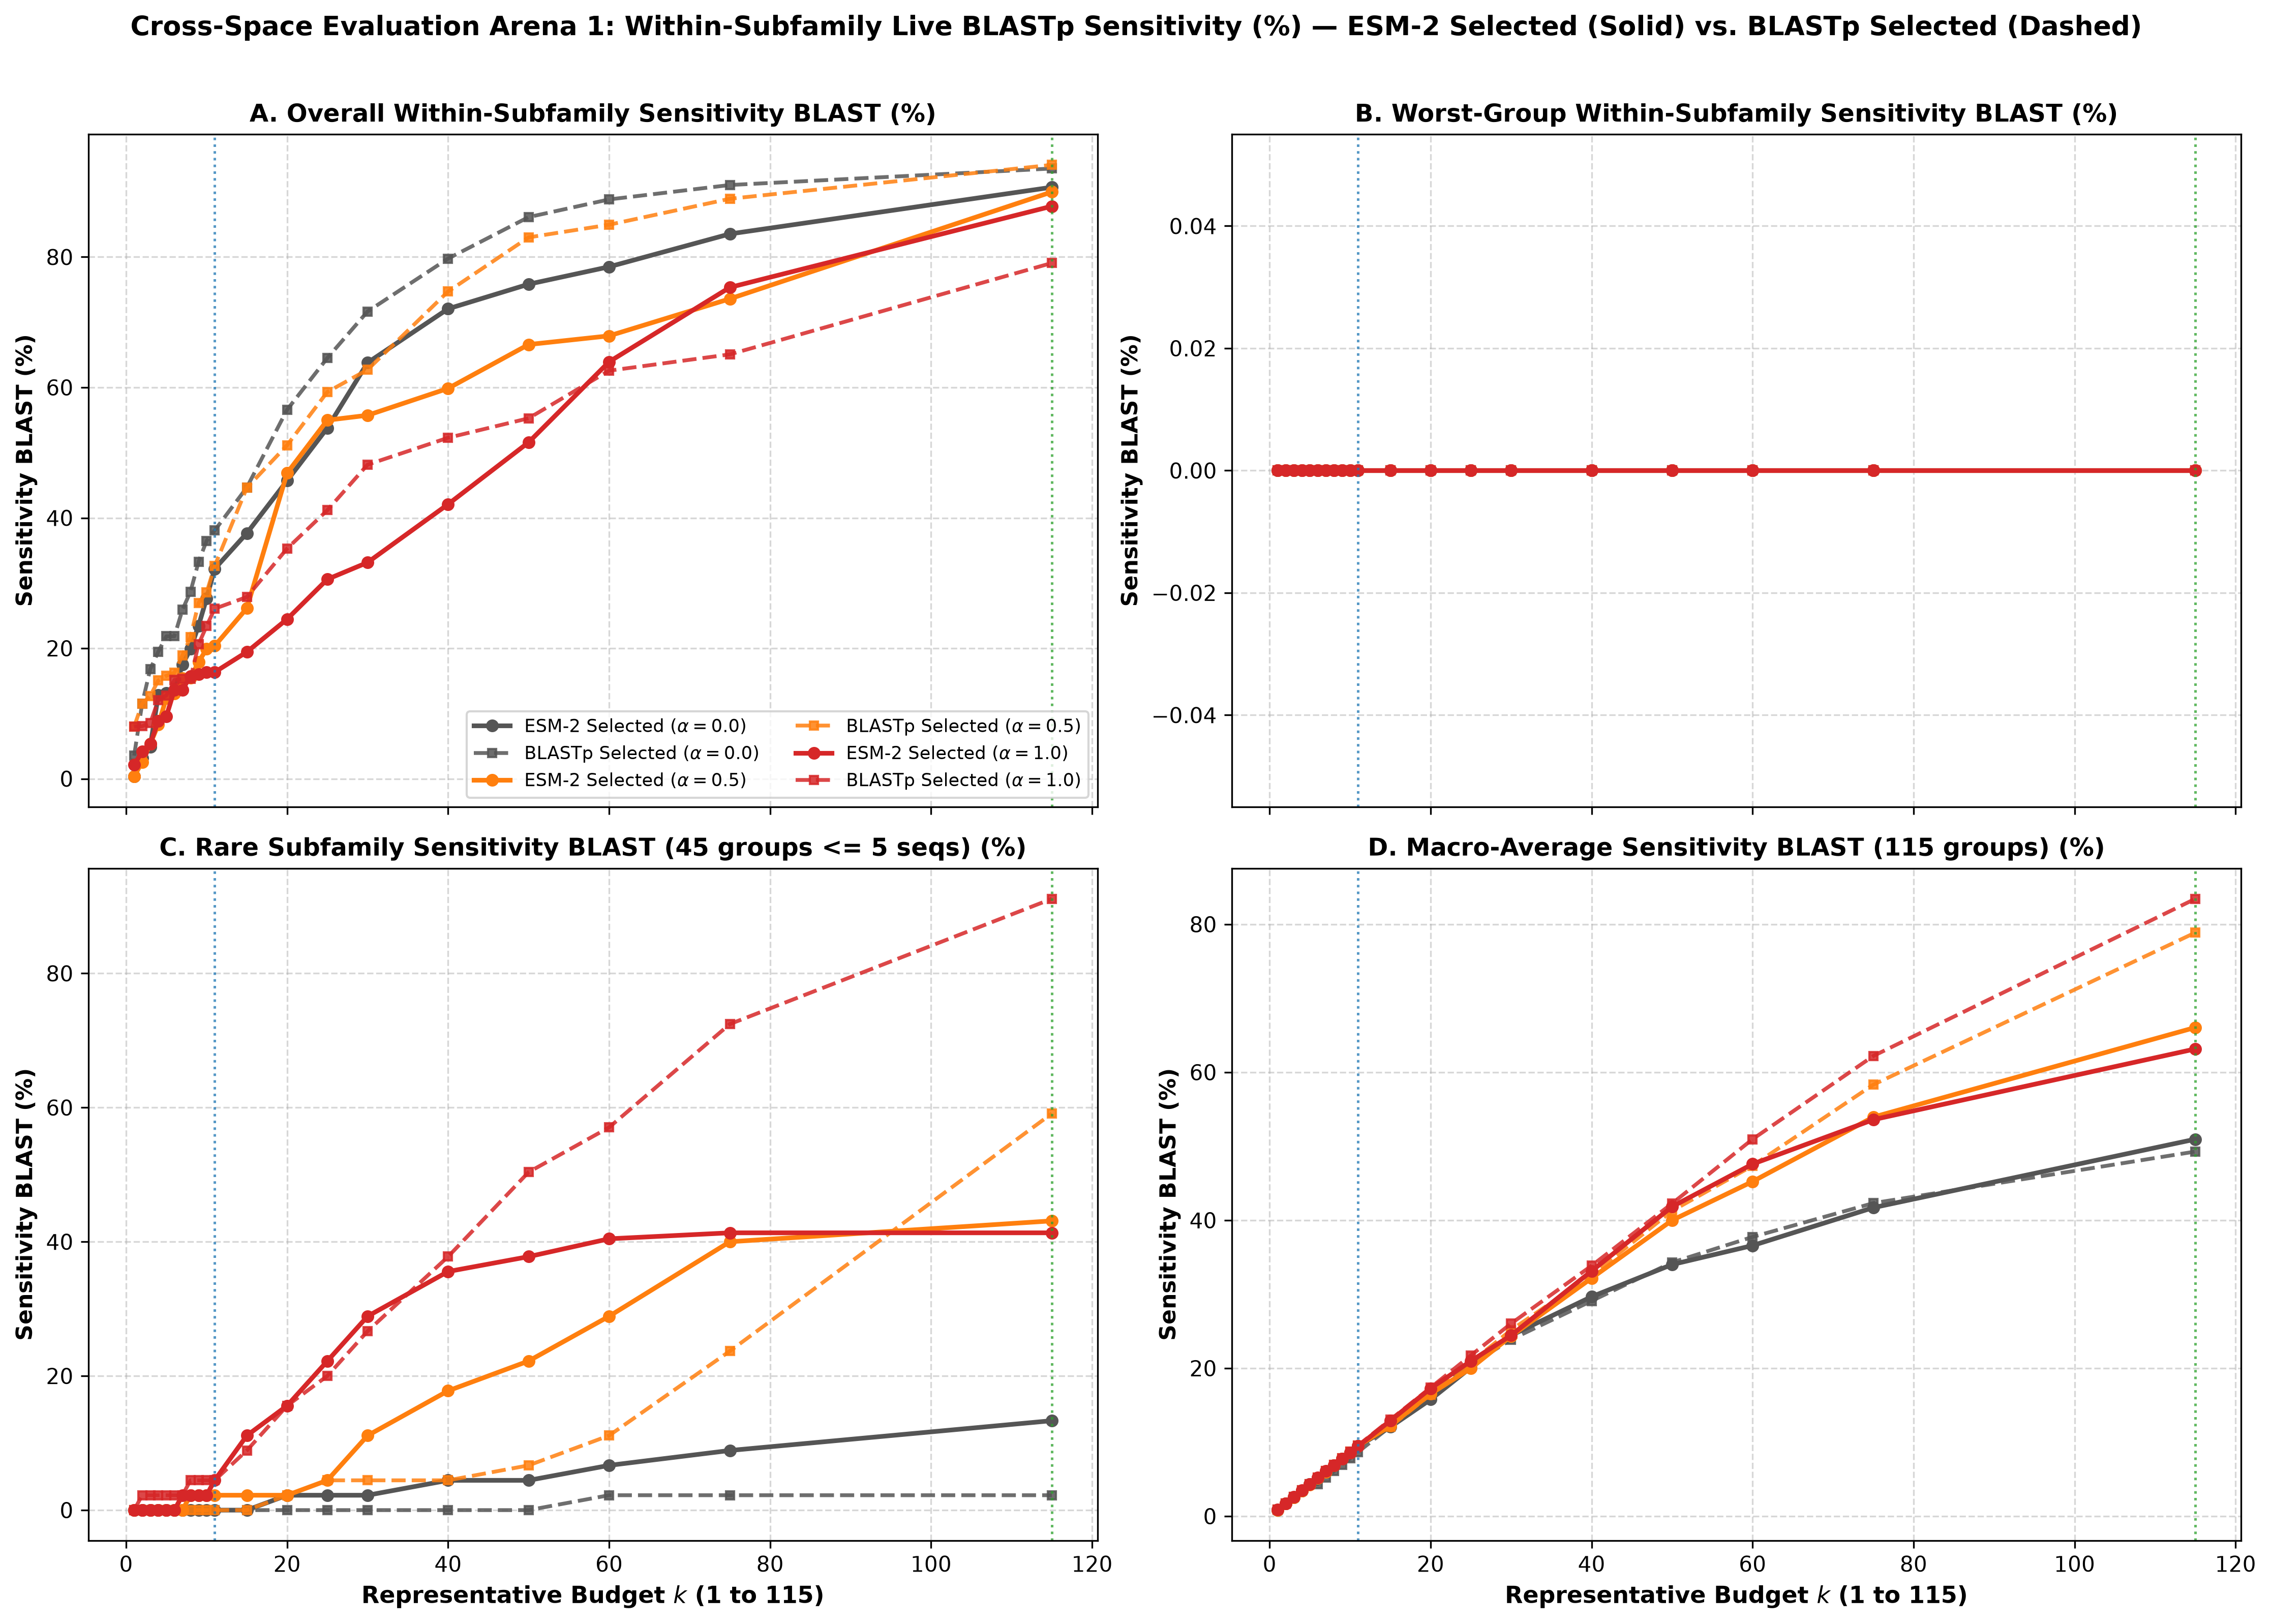
\includegraphics[width=0.92\textwidth]{Images/figures/exp4_blast_eval_comparison_vs_k.png}
    \caption{Hệ quy chiếu thứ nhất: so sánh hiệu năng giữa đại diện chọn bởi ESM-2 biểu diễn bằng đường nét liền và đại diện chọn bởi BLASTp biểu diễn bằng đường nét đứt trên thước đo Within-Subfamily Live BLASTp Sensitivity (\%) theo ngân sách $k \in [1..115]$.}
    \label{fig:exp4_blast_eval}
\end{figure}

\begin{figure}[htbp!]
    \centering
    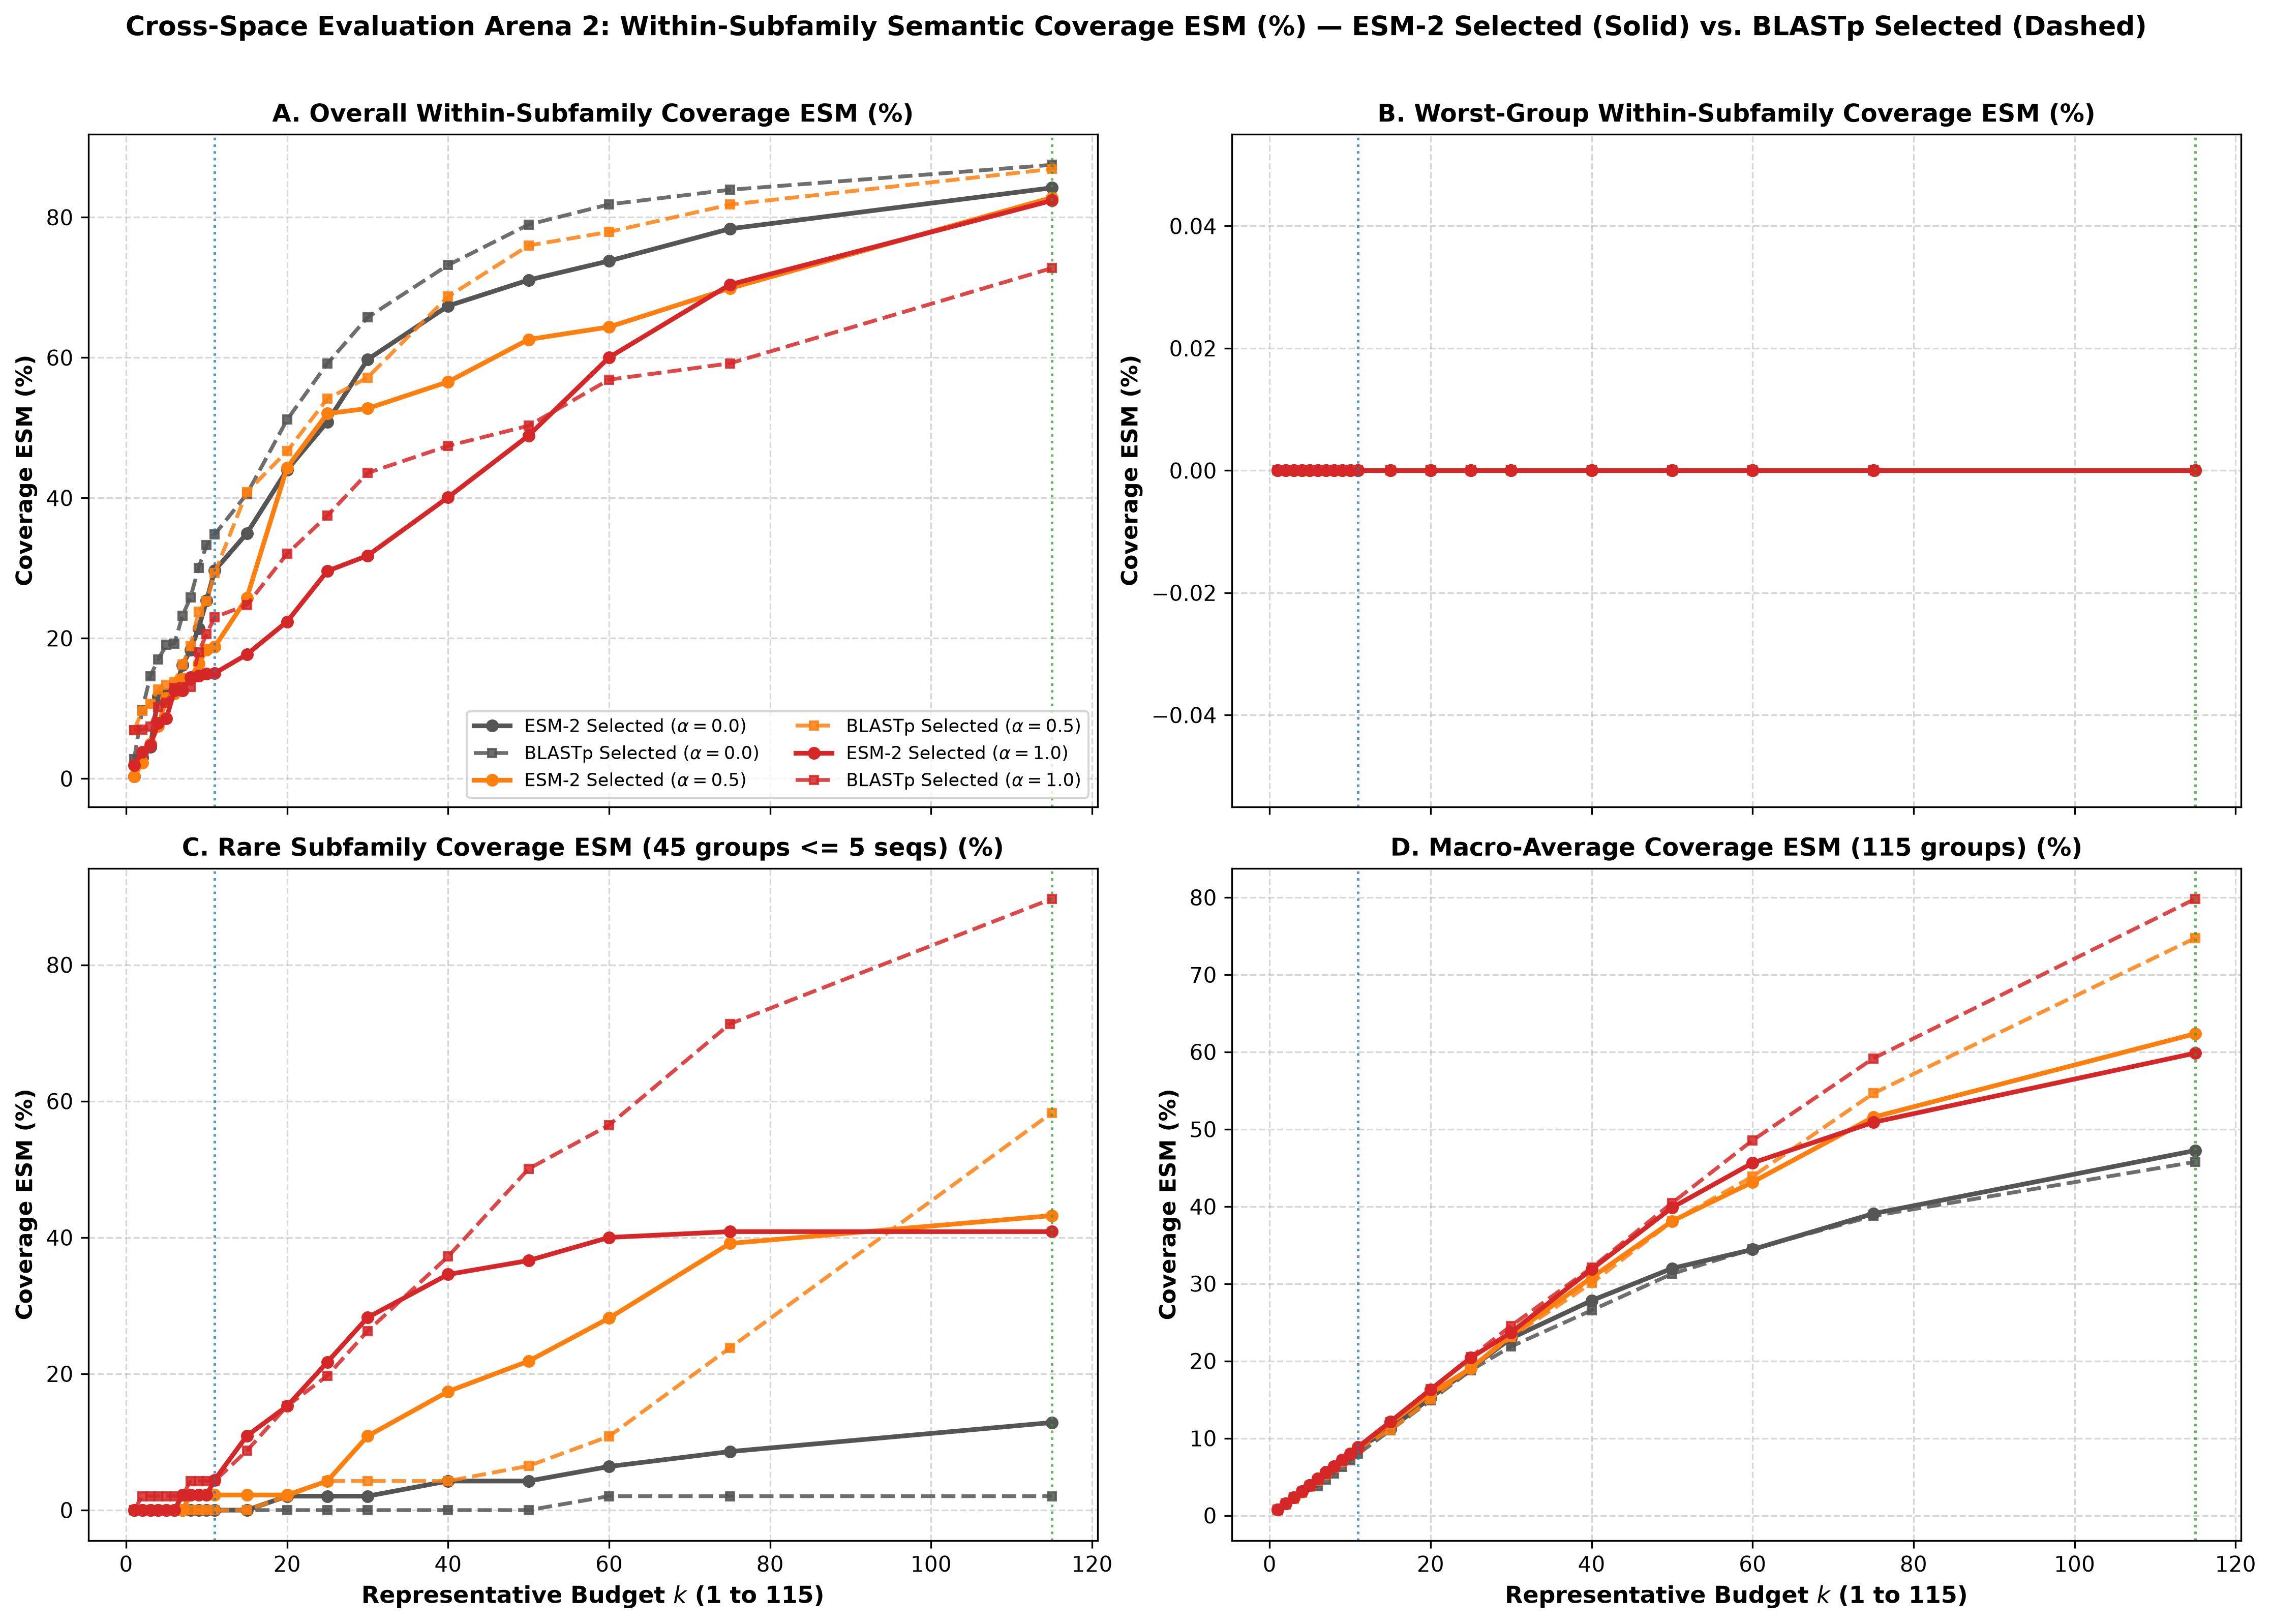
\includegraphics[width=0.92\textwidth]{Images/figures/exp4_esm_eval_comparison_vs_k.png}
    \caption{Hệ quy chiếu thứ hai: so sánh hiệu năng giữa đại diện chọn bởi ESM-2 biểu diễn bằng đường nét liền và đại diện chọn bởi BLASTp biểu diễn bằng đường nét đứt trên thước đo Within-Subfamily Coverage ESM (\%) theo ngân sách $k \in [1..115]$.}
    \label{fig:exp4_esm_eval}
\end{figure}

\FloatBarrier
Nguyên nhân toán học của sự đảo chiều về hiệu năng giữa hai không gian tại hình~\ref{fig:exp4_blast_eval}, hình~\ref{fig:exp4_esm_eval} và hình~\ref{fig:exp4_summary} bắt nguồn từ sự khác biệt cấu trúc giữa ma trận đặc ESM-2 và ma trận thưa BLASTp. Ma trận ngữ nghĩa $\mathbf{S}_{\text{ESM}}$ là ma trận đặc với $99{,}64\%$ cặp phần tử mang giá trị dương, giúp mỗi đại diện được chọn ở giai đoạn đầu ($k \le 75$) lan tỏa độ bao phủ sang các cụm lân cận và nhận diện sớm nhiều nhóm hiếm. Tuy nhiên, khi ngân sách tiến dần về $k = 115$, do mức tương đồng nền đã cao sẵn, phần độ tăng cận biên còn lại của các Subfamily hiếm bị thu hẹp và nhỏ hơn tổng độ tăng cận biên tích lũy trên hàng trăm chuỗi của các Subfamily lớn, khiến giải thuật ưu tiên chọn thêm đại diện cho nhóm lớn. Ngược lại, ma trận $\mathbf{S}_{\text{BLAST}}$ là ma trận thưa với độ tương đồng giữa các Subfamily xa nhau bằng $0{,}0$; khi các nhóm lớn đã được bao phủ nội bộ ở cuối dải ngân sách, độ tăng cận biên của chúng giảm về gần $0$, giúp các Subfamily hiếm chưa có đại diện giữ được độ tăng cận biên cao hơn và lần lượt được lựa chọn. Đặc biệt, tại mốc ngân sách trung bình $k = 60$, cấu hình BLASTp với trọng số mạnh $\alpha = 1{,}0$ đạt Rare Sensitivity lên tới $57{,}04\%$ và Overall Sensitivity đạt $62{,}57\%$, cao hơn so với ESM-2 $\alpha = 0{,}5$ ($28{,}89\%$ Rare Sensitivity, $67{,}91\%$ Overall Sensitivity) và ESM-2 $\alpha = 1{,}0$ ($40{,}44\%$ Rare Sensitivity, $63{,}93\%$ Overall Sensitivity). Như vậy, kiểm chứng chéo hai chiều cho thấy trọng số $\alpha = 0{,}5$ cải thiện tỷ lệ nhận diện nhóm hiếm trên cả hai không gian; trong đó không gian ESM-2 phát huy ưu thế bao phủ cụm ngữ nghĩa ở ngân sách vừa, còn không gian BLASTp với $\alpha \in \{0{,}5, 1{,}0\}$ bao phủ các phân họ hiếm đầy đủ hơn khi xét trên thước đo nhận diện chuỗi thực nghiệm Live BLASTp.

\begin{figure}[htbp!]
    \centering
    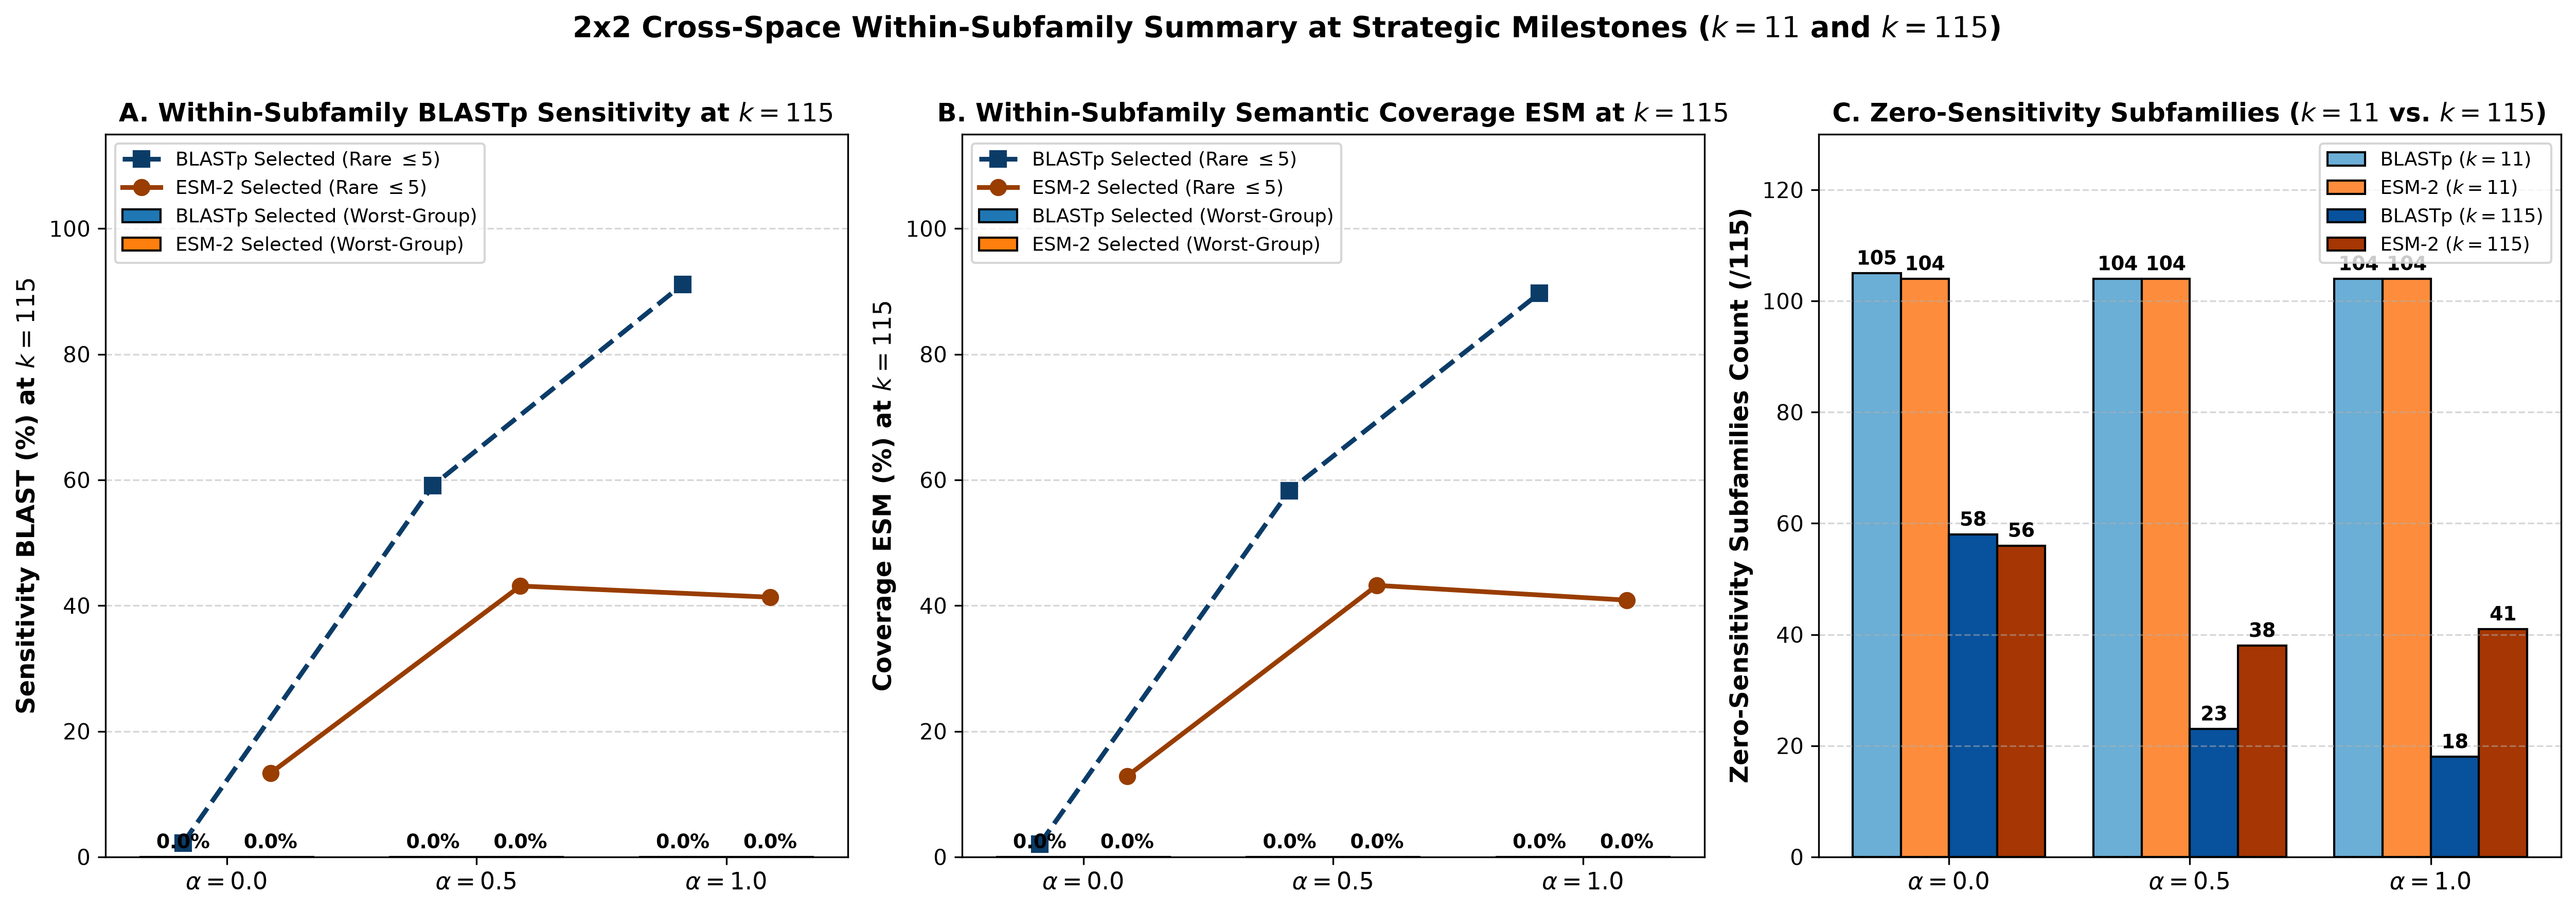
\includegraphics[width=0.92\textwidth]{Images/figures/exp4_cross_space_summary_k11_k76.png}
    \caption{Biểu đồ tổng hợp đối chiếu chéo hai chiều giữa đại diện chọn bởi BLASTp và đại diện chọn bởi ESM-2 tại hai mốc chiến lược $k = 11$ và $k = 115$.}
    \label{fig:exp4_summary}
\end{figure}

\FloatBarrier\section{Phân tích cơ chế phân bổ đại diện và khảo sát độ bão hòa khi mở rộng ngân sách}
\label{sec:allocation_saturation_discussion}
\phantomsection\label{sec:branch_5}
\phantomsection\label{subsec:branch5_invariants}
\phantomsection\label{subsec:branch5_results}

Nhằm làm rõ cơ chế vi mô giúp hàm mục tiêu có trọng số cải thiện đáng kể tỷ lệ nhận diện các phân họ hiếm mà không làm suy giảm độ bao phủ tổng thể, thử nghiệm 5 phân tích trực tiếp cơ cấu nhãn Subfamily của từng chuỗi đại diện bên trong tập nghiệm $S_k$ trên toàn bộ $120$ cấu hình thực nghiệm.

Kết quả phân tích chỉ ra rằng tại ngân sách $k = 115$, mô hình không trọng số ($\alpha = 0{,}0$) phân bổ lặp lại tới $58$ vị trí đại diện vào các Subfamily lớn đã có đại diện, đẩy chỉ số dư thừa phân bổ Subfamily Redundancy lên mức $50{,}43\%$ và khiến $58$ trên $115$ Subfamily không có đại diện. Ngược lại, tại cùng mốc ngân sách $k = 115$, RareProtSelect với trọng số $\alpha = 0{,}5$ giảm đáng kể độ dư thừa phân bổ từ $50{,}43\%$ xuống còn $20{,}00\%$, chuyển $35$ vị trí đại diện dư thừa từ các nhóm lớn sang phân bổ cho các phân họ chưa có đại diện, qua đó nâng số lượng Subfamily có đại diện lên $92$ trên $115$ phân họ chính thức ($80{,}00\%$) và $27$ trên $45$ Subfamily hiếm ($60{,}00\%$), đồng thời giảm một nửa tỷ trọng ngân sách của Subfamily lớn nhất A01.009 từ $6$ vị trí ($5{,}22\%$) ở $\alpha = 0{,}0$ xuống chỉ còn $3$ vị trí ($2{,}61\%$) ở $\alpha = 0{,}5$, và tương tự tại $k = 11$ giảm từ $18{,}18\%$ xuống $9{,}09\%$. Bảng~\ref{tab:exp5_milestones} tổng hợp số liệu đo đạc cấu trúc phân bổ tại các mốc ngân sách đại diện.

\begin{table}[htbp!]
\centering
\caption{Phân bổ cấu trúc vị trí đại diện, tỷ lệ đại diện nhóm hiếm và độ dư thừa phân bổ trong tập nghiệm $S_k$ tại các mốc ngân sách đại diện.}
\label{tab:exp5_milestones}
\vspace{4pt}
\small
\resizebox{\textwidth}{!}{%
\begin{tabular}{cccrrrrr}
\toprule
\textbf{Không gian} & \textbf{Hệ số $\alpha$} & \textbf{Ngân sách $k$} & \textbf{Subfamily Representation} & \textbf{Rare Representation} & \textbf{Subfamily Redundancy} & \textbf{Vị trí A01.009} & \textbf{Tỷ trọng A01.009} \\
\midrule
BLASTp & 0{,}0 & $k = 11$  & 10 / 115 (8{,}70\%) & 0 / 45 (0{,}0\%)  & 1 (9{,}09\%)  & 2 & 18{,}18\% \\
ESM-2  & 0{,}0 & $k = 11$  & 11 / 115 (9{,}57\%) & 0 / 45 (0{,}0\%)  & 0 (0{,}0\%)   & 1 & 9{,}09\% \\
BLASTp & 0{,}5 & $k = 11$  & 11 / 115 (9{,}57\%) & 0 / 45 (0{,}0\%)  & 0 (0{,}0\%)   & 1 & 9{,}09\% \\
ESM-2  & 0{,}5 & $k = 11$  & 11 / 115 (9{,}57\%) & 1 / 45 (2{,}22\%) & 0 (0{,}0\%)   & 0 & 0{,}00\% \\
\midrule
BLASTp & 0{,}0 & $k = 50$  & 40 / 115 (34{,}78\%)& 0 / 45 (0{,}0\%)  & 10 (20{,}0\%) & 4 & 8{,}00\% \\
BLASTp & 0{,}5 & $k = 50$  & 48 / 115 (41{,}74\%)& 3 / 45 (6{,}67\%) & 2 (4{,}0\%)   & 2 & 4{,}00\% \\
ESM-2  & 0{,}5 & $k = 50$  & 47 / 115 (40{,}87\%)& 10 / 45 (22{,}22\%)& 3 (6{,}0\%)  & 1 & 2{,}00\% \\
\midrule
BLASTp & 0{,}0 & $k = 115$ & 57 / 115 (49{,}57\%)& 1 / 45 (2{,}22\%) & 58 (50{,}43\%)& 6 & 5{,}22\% \\
BLASTp & 0{,}5 & $k = 115$ & \textbf{92 / 115 (80{,}00\%)}& \textbf{27 / 45 (60{,}00\%)}& \textbf{23 (20{,}00\%)}& \textbf{3} & \textbf{2{,}61\%} \\
BLASTp & 1{,}0 & $k = 115$ & \textbf{97 / 115 (84{,}35\%)}& \textbf{41 / 45 (91{,}11\%)}& \textbf{18 (15{,}65\%)}& \textbf{2} & \textbf{1{,}74\%} \\
ESM-2  & 0{,}5 & $k = 115$ & 77 / 115 (66{,}96\%)& 20 / 45 (44{,}44\%)& 38 (33{,}04\%)& 4 & 3{,}48\% \\
ESM-2  & 1{,}0 & $k = 115$ & 74 / 115 (64{,}35\%)& 19 / 45 (42{,}22\%)& 41 (35{,}65\%)& 1 & 0{,}87\% \\
\bottomrule
\end{tabular}%
}
\end{table}

Bảng~\ref{tab:exp5_milestones} làm sáng tỏ cơ chế vi mô của sự phân bổ: ở mô hình cơ sở $\alpha = 0{,}0$ tại $k = 115$, có tới $58$ vị trí đại diện bị trùng lặp Subfamily với độ dư thừa lên tới $50{,}43\%$, khiến chỉ có $57$ Subfamily được đại diện và để sót $44$ trên $45$ Subfamily hiếm. Thiết lập $\alpha = 0{,}5$ và $\alpha = 1{,}0$ tái phân bổ hiệu quả ngân sách, trong đó $\alpha = 0{,}5$ đạt $92/115$ ($80{,}00\%$) Subfamily có đại diện và $\alpha = 1{,}0$ đạt $97/115$ ($84{,}35\%$) Subfamily có đại diện trên BLASTp (và $74/115$, tức $64{,}35\%$ trên ESM-2). Cần lưu ý rằng nếu nhãn phân họ đã biết trước tại mốc đúng bằng số phân họ $k = G = 115$, một chiến lược hạn mức cứng đơn giản (1-medoid-per-subfamily) có thể hiển nhiên đạt $100\%$ đại diện phân họ ($115/115$) và $100\%$ đại diện nhóm hiếm ($45/45$). Tuy nhiên, chiến lược cứng đó không có hàm mục tiêu liên tục để xếp hạng ưu tiên các phân họ quan trọng khi ngân sách nhỏ hơn số phân họ ($k \ll G$), và cũng không thể tự động phân bổ thêm đại diện tương ứng với độ phân kỳ nội họ khi ngân sách mở rộng ($k > G$). Hàm mục tiêu submodular có trọng số $F_\alpha(S)$ giải quyết bài toán tối ưu hóa liên tục trên toàn dải ngân sách $k$, dù tại $k = 115$, do tương đồng chéo $\mathbf{S}(u, v) > 0$ và biến dị nội nhóm của các phân họ lớn, $\alpha = 1{,}0$ vẫn phân bổ $18$ vị trí đại diện trên BLASTp và $41$ vị trí đại diện trên ESM-2 cho các đại diện thứ hai của nhóm lớn thay vì bao phủ đủ $115$ phân họ.

\begin{figure}[htbp!]
    \centering
    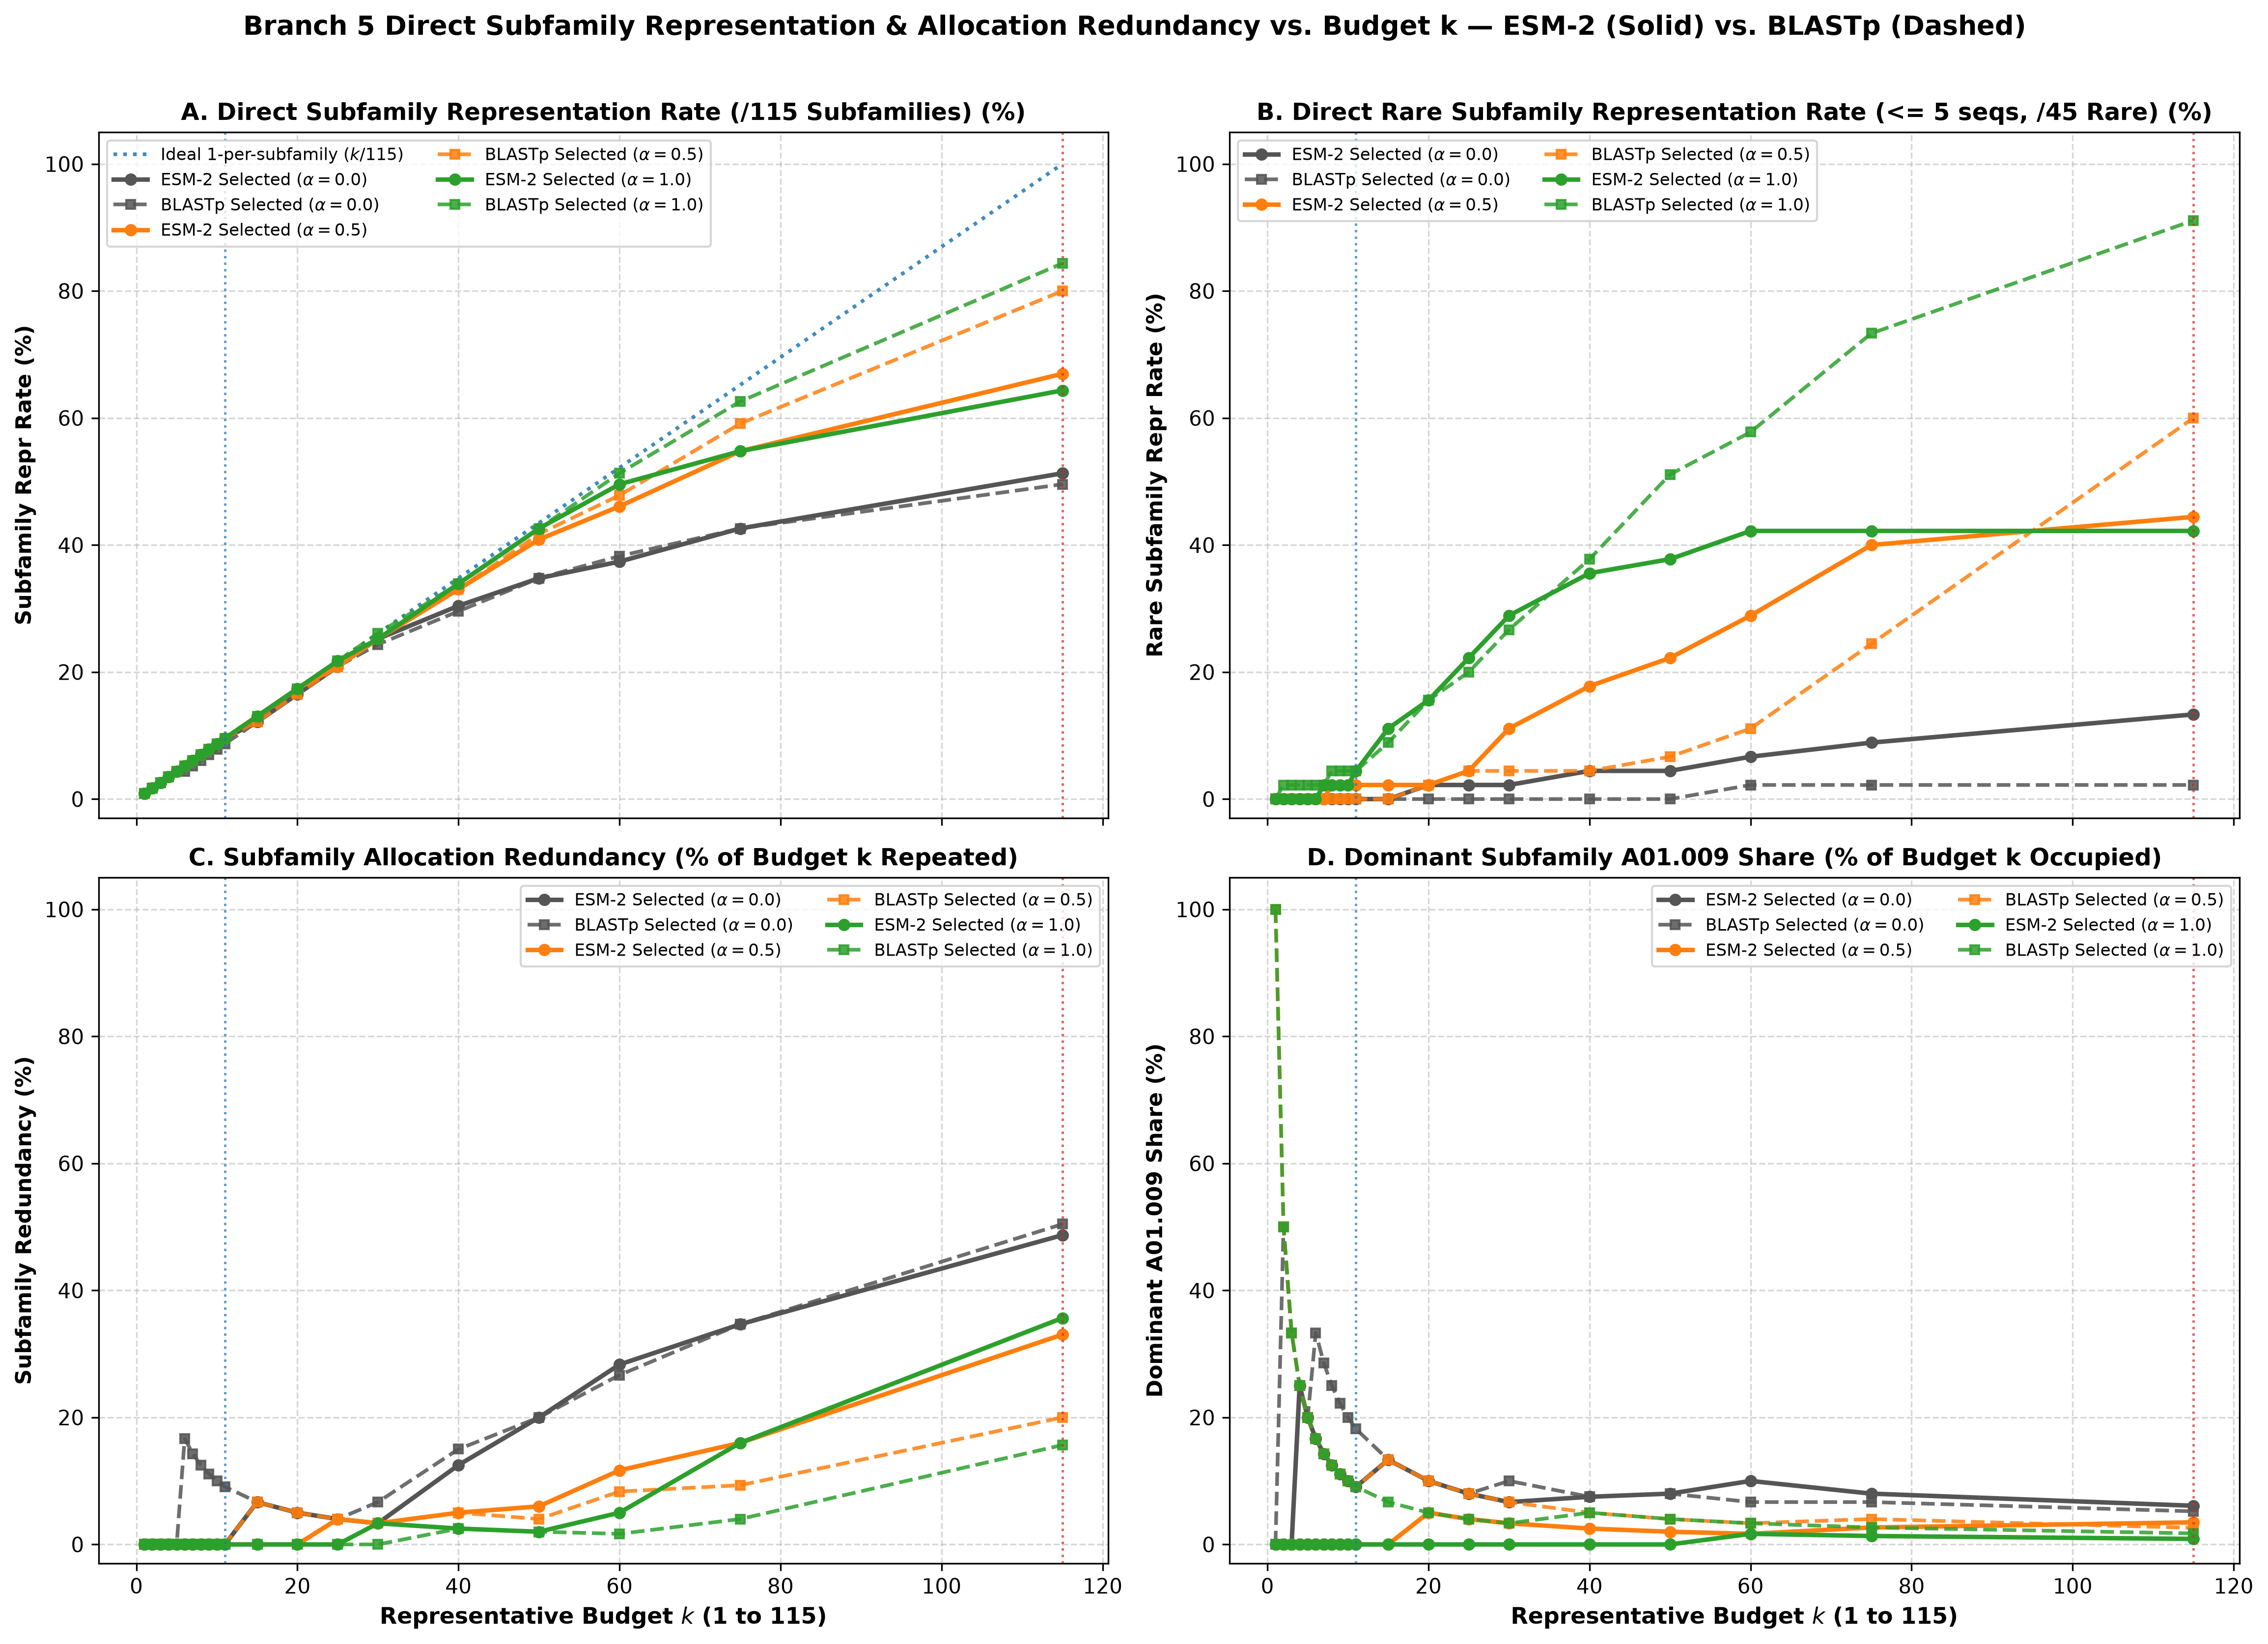
\includegraphics[width=0.92\textwidth]{Images/figures/exp5_allocation_metrics_vs_k.png}
    \caption{Sự biến thiên của bốn chỉ số cấu trúc phân bổ đại diện và tỷ lệ dư thừa theo ngân sách $k \in [1..115]$ giữa ESM-2 biểu diễn bằng đường nét liền và BLASTp biểu diễn bằng đường nét đứt qua ba mức $\alpha$.}
    \label{fig:exp5_allocation}
\end{figure}

\begin{figure}[htbp!]
    \centering
    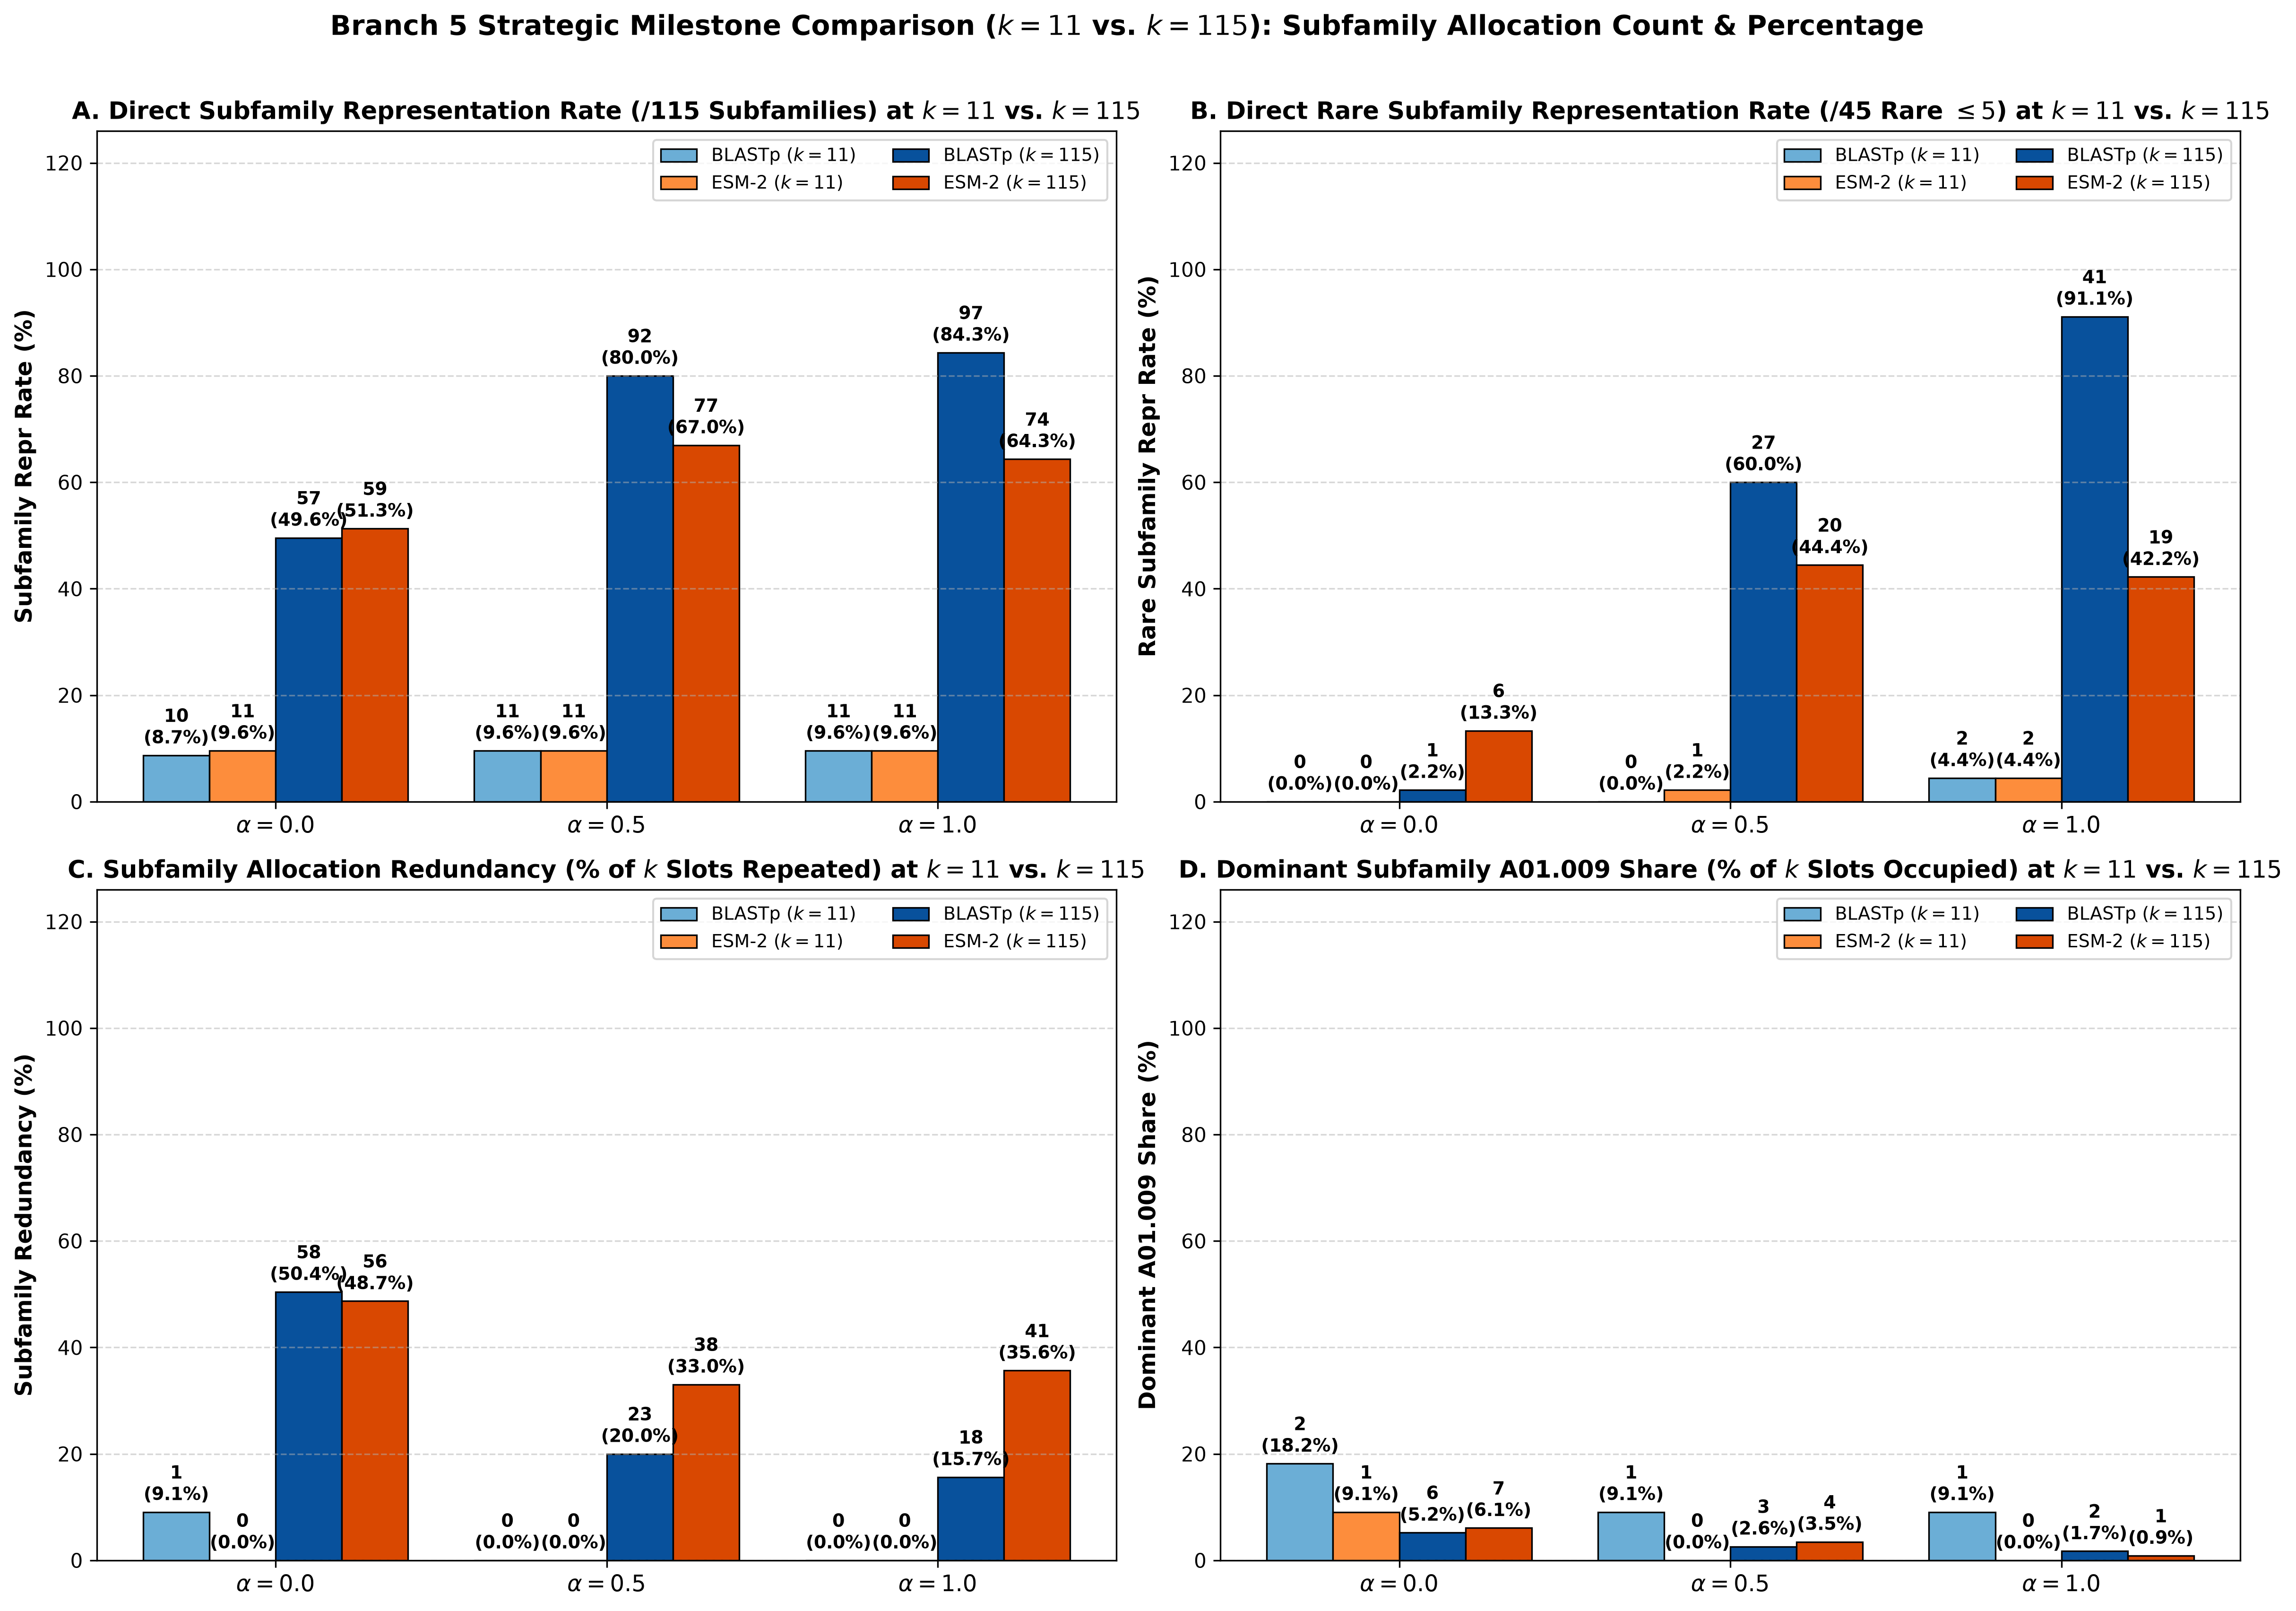
\includegraphics[width=0.92\textwidth]{Images/figures/exp5_allocation_summary_k11_k76.png}
    \caption{Biểu đồ cột ghép đối chiếu cấu trúc đại diện phân họ, đại diện nhóm hiếm, độ dư thừa và tỷ trọng đại diện của Subfamily A01.009 tại hai mốc $k = 11$ và $k = 115$.}
    \label{fig:exp5_summary}
\end{figure}

Hình~\ref{fig:exp5_allocation} và hình~\ref{fig:exp5_summary} cung cấp bằng chứng định lượng rõ ràng cho thấy phương pháp RareProtSelect hóa giải hiệu quả sự thiên lệch quy mô mẫu và tái cân bằng mức ưu tiên tối ưu hóa cho các Subfamily hiếm.

\phantomsection\label{subsec:branch6_deep_budget}

Ở các thử nghiệm trước, ngân sách tối đa được giới hạn ở ngưỡng đối chuẩn $k \le G = 115$, tương ứng tỷ lệ bình quân một đại diện trên mỗi phân họ. Tại ngưỡng này, hàm mục tiêu có trọng số $\alpha = 0{,}5$ ưu tiên ngân sách để bảo vệ các Subfamily hiếm, dẫn đến việc Subfamily lớn nhất A01.009 chỉ nhận được $3$ đại diện và chưa đạt độ bao phủ tối đa. Đối với một họ protein có độ đa dạng cao và phân tách thành nhiều phân họ với quy mô chênh lệch lớn như Family A1, ngân sách cơ sở $k = 115$ là chưa đủ để đồng thời bao phủ hết các Subfamily hiếm lẫn sự biến dị trình tự axit amin bên trong các Subfamily lớn. Do đó, thử nghiệm 6 mở rộng ngân sách lên $k_{\max} = 380$ chuỗi nhằm khảo sát quá trình hội tụ độ bao phủ của các phân họ lớn và toàn bộ siêu họ khi tăng số lượng đại diện.

Sáu mốc ngân sách chiến lược $k \in \{115, 150, 200, 270, 340, 380\}$ được thiết kế dựa trên cấu trúc phân tầng quy mô của $115$ Subfamily chính thức gồm $45$ Subfamily hiếm có $n_g \le 5$ chuỗi, $32$ Subfamily trung bình có $6 \le n_g \le 19$ chuỗi và $38$ Subfamily lớn có $n_g \ge 20$ chuỗi. Cụ thể, mốc $k = 115$ là ngưỡng ngân sách cơ sở tương ứng bình quân một đại diện cho mỗi phân họ; hai mốc $k = 150$ và $k = 200$ mở rộng thêm lần lượt $35$ và $50$ vị trí nhằm phân bổ thêm đại diện thứ hai và thứ ba cho $38$ Subfamily lớn; hai mốc $k = 270$ và $k = 340$ tăng thêm mỗi bước $70$ vị trí, tương ứng tổng số $38$ nhóm lớn và $32$ nhóm trung bình, để bổ sung đại diện thứ hai, thứ ba cho các phân họ trung bình và đại diện thứ tư, thứ năm cho các phân họ lớn; cuối cùng, mốc $k = 380$ bổ sung thêm $40$ vị trí nhằm phân bổ đại diện thứ sáu cho khối phân họ lớn, qua đó đánh giá mức độ hội tụ độ bao phủ ở vùng ngân sách cao.

Cần lưu ý một khác biệt về thiết lập tham số giữa ngưỡng ngân sách tối đa của thử nghiệm 6 và các thử nghiệm trước: tại thử nghiệm 2 và thử nghiệm 5, cơ chế xác lập thứ hạng đồng thuận qua $M = 1.000$ lần xáo trộn ngẫu nhiên độc lập được chạy với ngưỡng ngân sách tối đa $k_{\max} = 115$, ghi nhận $92$ Subfamily có đại diện và chỉ số Rare Sensitivity đạt $59{,}11\%$. Trong khi đó, tại thử nghiệm 6, quy trình đồng thuận được thiết lập trên ngưỡng ngân sách mở rộng $k_{\max} = 380$, dẫn đến sự thay đổi nhẹ về thứ tự chọn giữa các ứng viên chuỗi có độ tăng cận biên tương đương trong các lượt xáo trộn ngẫu nhiên. Vì vậy, lát cắt quan sát tại mốc $k = 115$ của cấu hình $k_{\max} = 380$ ghi nhận $88$ Subfamily có đại diện và Rare Sensitivity đạt $50{,}22\%$. Sự khác biệt này phản ánh đặc tính của cơ chế xếp hạng đồng thuận khi thay đổi số bước tích lũy $k_{\max}$, nhưng vẫn giữ nguyên xu hướng hội tụ bão hòa tổng thể.

Kết quả đo đạc thực nghiệm tại bảng~\ref{tab:exp6_milestones} cho thấy khi mở rộng ngân sách đến $k = 380$, tập đại diện trên không gian BLASTp nhận diện được chuỗi của $112$ trên $115$ Subfamily ($97{,}39\%$), trong đó có $104$ Subfamily đạt tỷ lệ nhận diện $100\%$ Sensitivity; đồng thời Subfamily lớn nhất A01.009 được phân bổ $6$ vị trí đại diện trên BLASTp và $22$ vị trí đại diện trên ESM-2, giúp độ bao phủ nội phân họ tiệm cận mức tối đa.

\begin{table}[htbp!]
\centering
\caption{Mức độ bão hòa độ bao phủ theo từng nhóm quy mô phân họ và số vị trí đại diện của Subfamily A01.009 khi mở rộng ngân sách lên $k \in [115..380]$ với $\alpha = 0{,}5$.}
\label{tab:exp6_milestones}
\vspace{4pt}
\small
\resizebox{\textwidth}{!}{%
\begin{tabular}{ccrrrrrr}
\toprule
\textbf{Không gian} & \textbf{Ngân sách $k$} & \textbf{Subfamily Representation} & \textbf{Vị trí A01.009} & \textbf{Common Sensitivity} & \textbf{Medium Sensitivity} & \textbf{Rare Sensitivity} & \textbf{Full Saturation (100\%)} \\
\midrule
BLASTp & $k = 115$ & 88 (76{,}52\%)  & 3 (2{,}61\%) & 96{,}47\% & 85{,}75\% & 50{,}22\% & 78 / 115 \\
BLASTp & $k = 150$ & 97 (84{,}35\%)  & 4 (2{,}67\%) & 99{,}13\% & 92{,}00\% & 64{,}00\% & 86 / 115 \\
BLASTp & $k = 200$ & 102 (88{,}70\%) & 4 (2{,}00\%) & 99{,}26\% & 96{,}69\% & 73{,}33\% & 93 / 115 \\
BLASTp & $k = 270$ & 107 (93{,}04\%) & 5 (1{,}85\%) & 99{,}32\% & 99{,}82\% & 82{,}22\% & 98 / 115 \\
BLASTp & $k = 340$ & 108 (93{,}91\%) & 6 (1{,}76\%) & 99{,}41\% & 100{,}00\% & 84{,}44\% & 100 / 115 \\
BLASTp & $k = 380$ & \textbf{112 (97{,}39\%)}& \textbf{6 (1{,}58\%)} & \textbf{99{,}41\%} & \textbf{100{,}00\%} & \textbf{93{,}33\%} & \textbf{104 / 115} \\
\midrule
ESM-2  & $k = 115$ & 77 (66{,}96\%)  & 4 (3{,}48\%) & 91{,}31\% & 68{,}30\% & 43{,}11\% & 69 / 115 \\
ESM-2  & $k = 150$ & 81 (70{,}43\%)  & 5 (3{,}33\%) & 94{,}00\% & 77{,}68\% & 43{,}56\% & 73 / 115 \\
ESM-2  & $k = 200$ & 82 (71{,}30\%)  & 5 (2{,}50\%) & 96{,}63\% & 77{,}68\% & 43{,}56\% & 74 / 115 \\
ESM-2  & $k = 270$ & 82 (71{,}30\%)  & 7 (2{,}59\%) & 96{,}93\% & 77{,}68\% & 43{,}56\% & 75 / 115 \\
ESM-2  & $k = 340$ & 85 (73{,}91\%)  & 21 (6{,}18\%)& 96{,}95\% & 80{,}80\% & 48{,}00\% & 79 / 115 \\
ESM-2  & $k = 380$ & \textbf{95 (82{,}61\%)} & \textbf{22 (5{,}79\%)}& \textbf{96{,}95\%} & \textbf{82{,}37\%} & \textbf{68{,}00\%} & \textbf{88 / 115} \\
\bottomrule
\end{tabular}%
}
\end{table}

Số liệu tại bảng~\ref{tab:exp6_milestones} cùng các đồ thị tại hình~\ref{fig:exp6_dominant}, hình~\ref{fig:exp6_stratified} và hình~\ref{fig:exp6_saturation} cho thấy đối với một họ protein có độ đa dạng cao và phân tách thành nhiều phân họ như Family A1, việc mở rộng ngân sách vượt ngưỡng $k = 115$ giúp giải quyết sự cạnh tranh vị trí đại diện giữa các tầng quy mô. Phân họ lớn nhất A01.009 vốn đã đạt $100{,}0\%$ Sensitivity nội phân họ ngay từ mốc ngân sách $k = 115$ với $3$ chuỗi đại diện trên BLASTp và $4$ chuỗi đại diện trên ESM-2. Khi mở rộng ngân sách lên $k = 380$, việc tăng lên $6$ chuỗi trên BLASTp và $22$ chuỗi trên ESM-2 giúp nâng cao độ bao phủ hình học ngữ nghĩa liên tục ESM của riêng phân họ này từ $91{,}88\%$ lên $93{,}67\%$ trên BLASTp và từ $93{,}27\%$ lên $95{,}81\%$ trên ESM-2. Đồng thời, thuật toán nâng tỷ lệ nhận diện của khối phân họ hiếm từ $50{,}22\%$ lên $93{,}33\%$, đưa toàn bộ $32$ Subfamily trung bình đạt bão hòa $100{,}00\%$ Sensitivity và $38$ Subfamily lớn đạt bình quân $99{,}41\%$ Sensitivity trên không gian BLASTp. Kết quả này chứng minh khi được cung cấp ngân sách mở rộng, hàm mục tiêu có trọng số $\alpha = 0{,}5$ vừa bao phủ rộng khắp các phân họ hiếm, vừa mở rộng độ bao phủ biến dị nội nhóm cho các phân họ quy mô lớn.

\begin{figure}[htbp!]
    \centering
    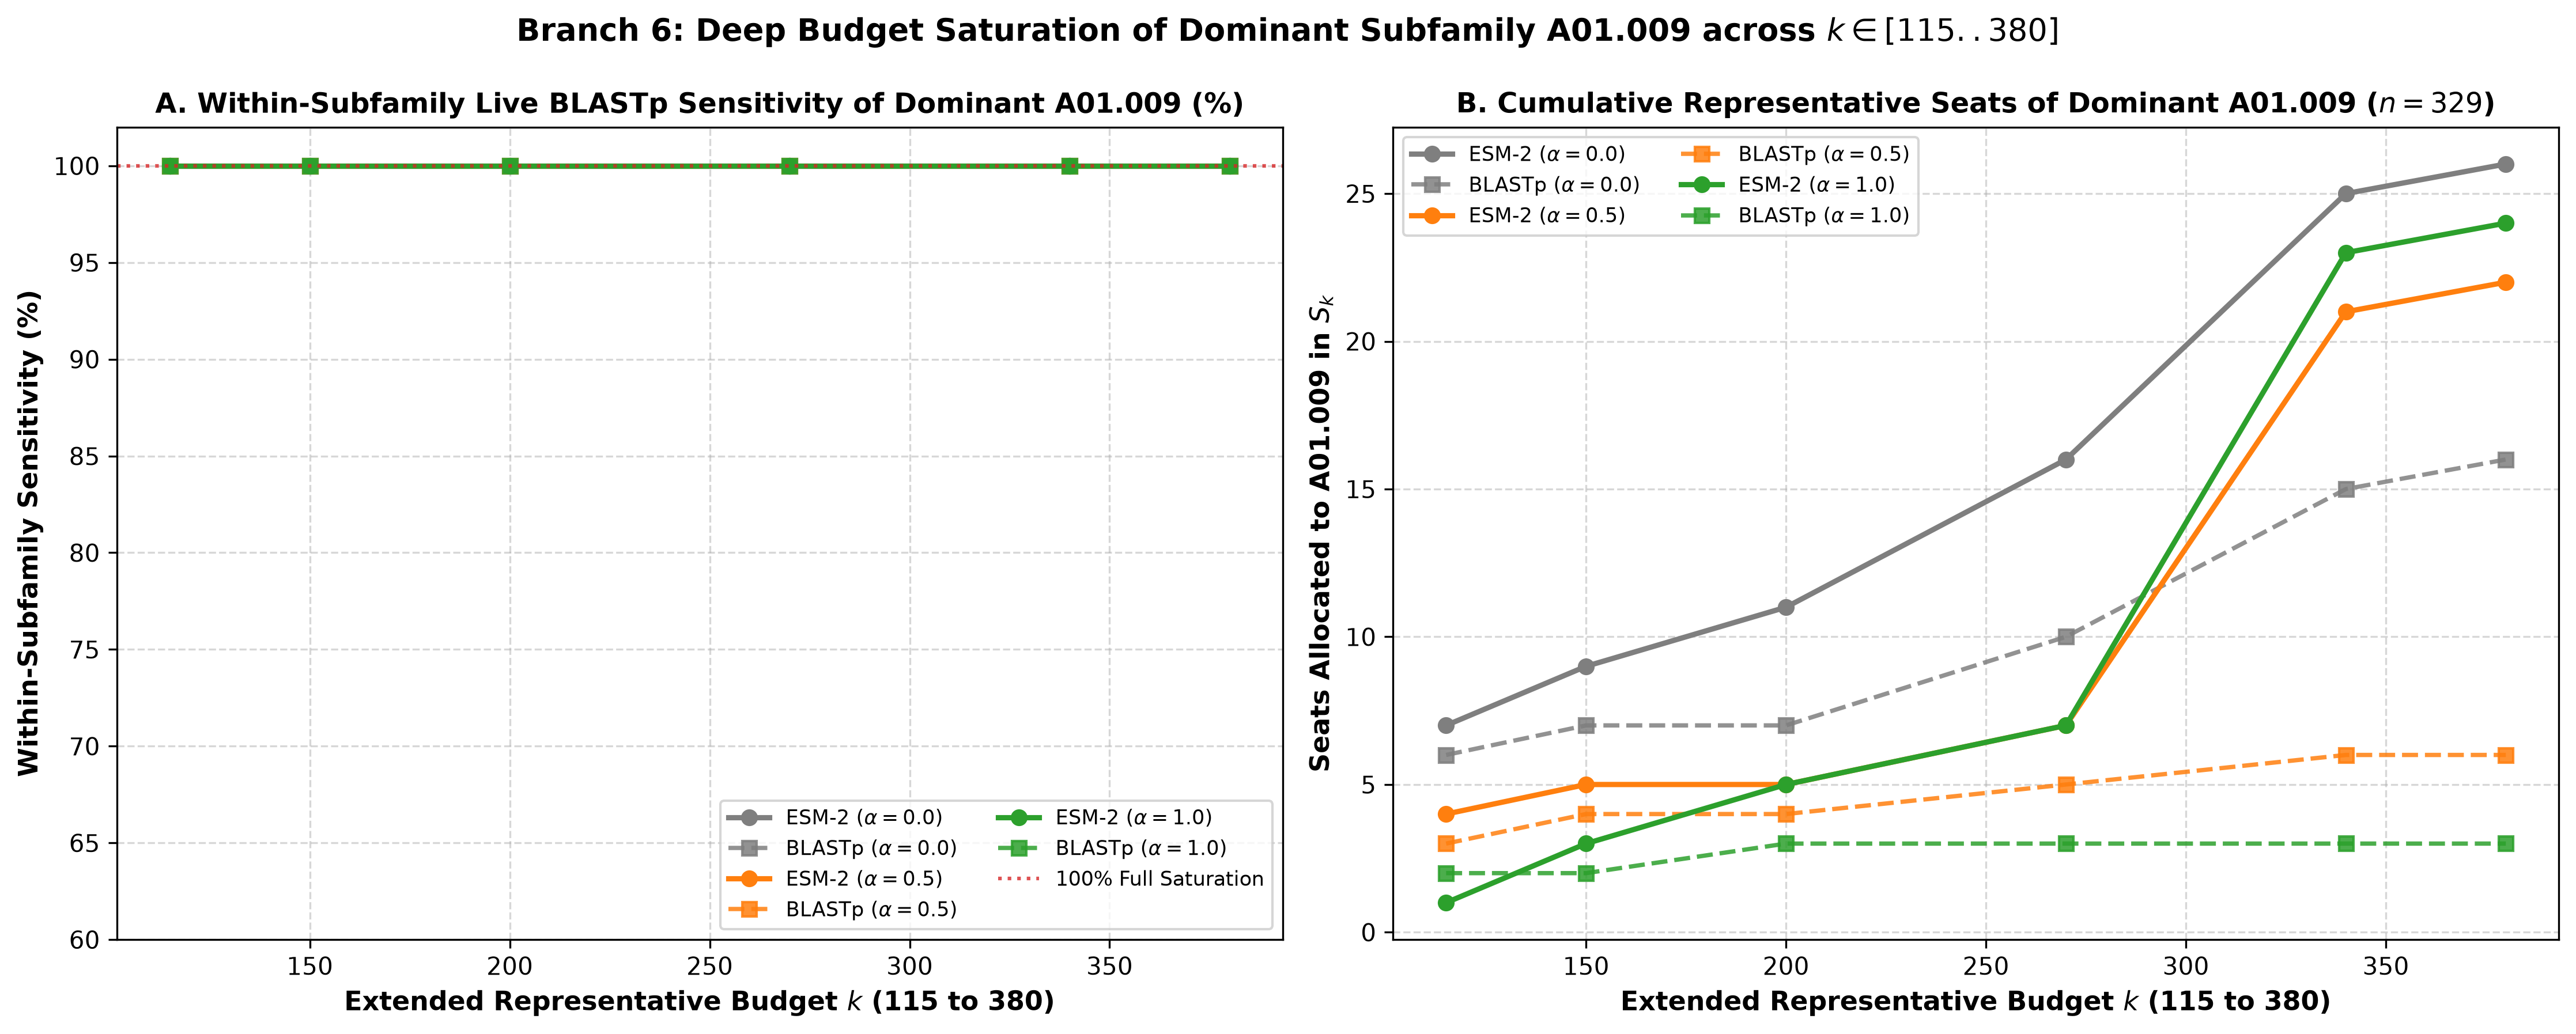
\includegraphics[width=0.92\textwidth]{Images/figures/exp6_dominant_a01_009_saturation_vs_k.png}
    \caption{Sự tích lũy số lượng đại diện và quá trình bão hòa độ bao phủ nội phân họ của Subfamily lớn nhất A01.009 khi mở rộng ngân sách lên $k \in [115..380]$.}
    \label{fig:exp6_dominant}
\end{figure}

\begin{figure}[htbp!]
    \centering
    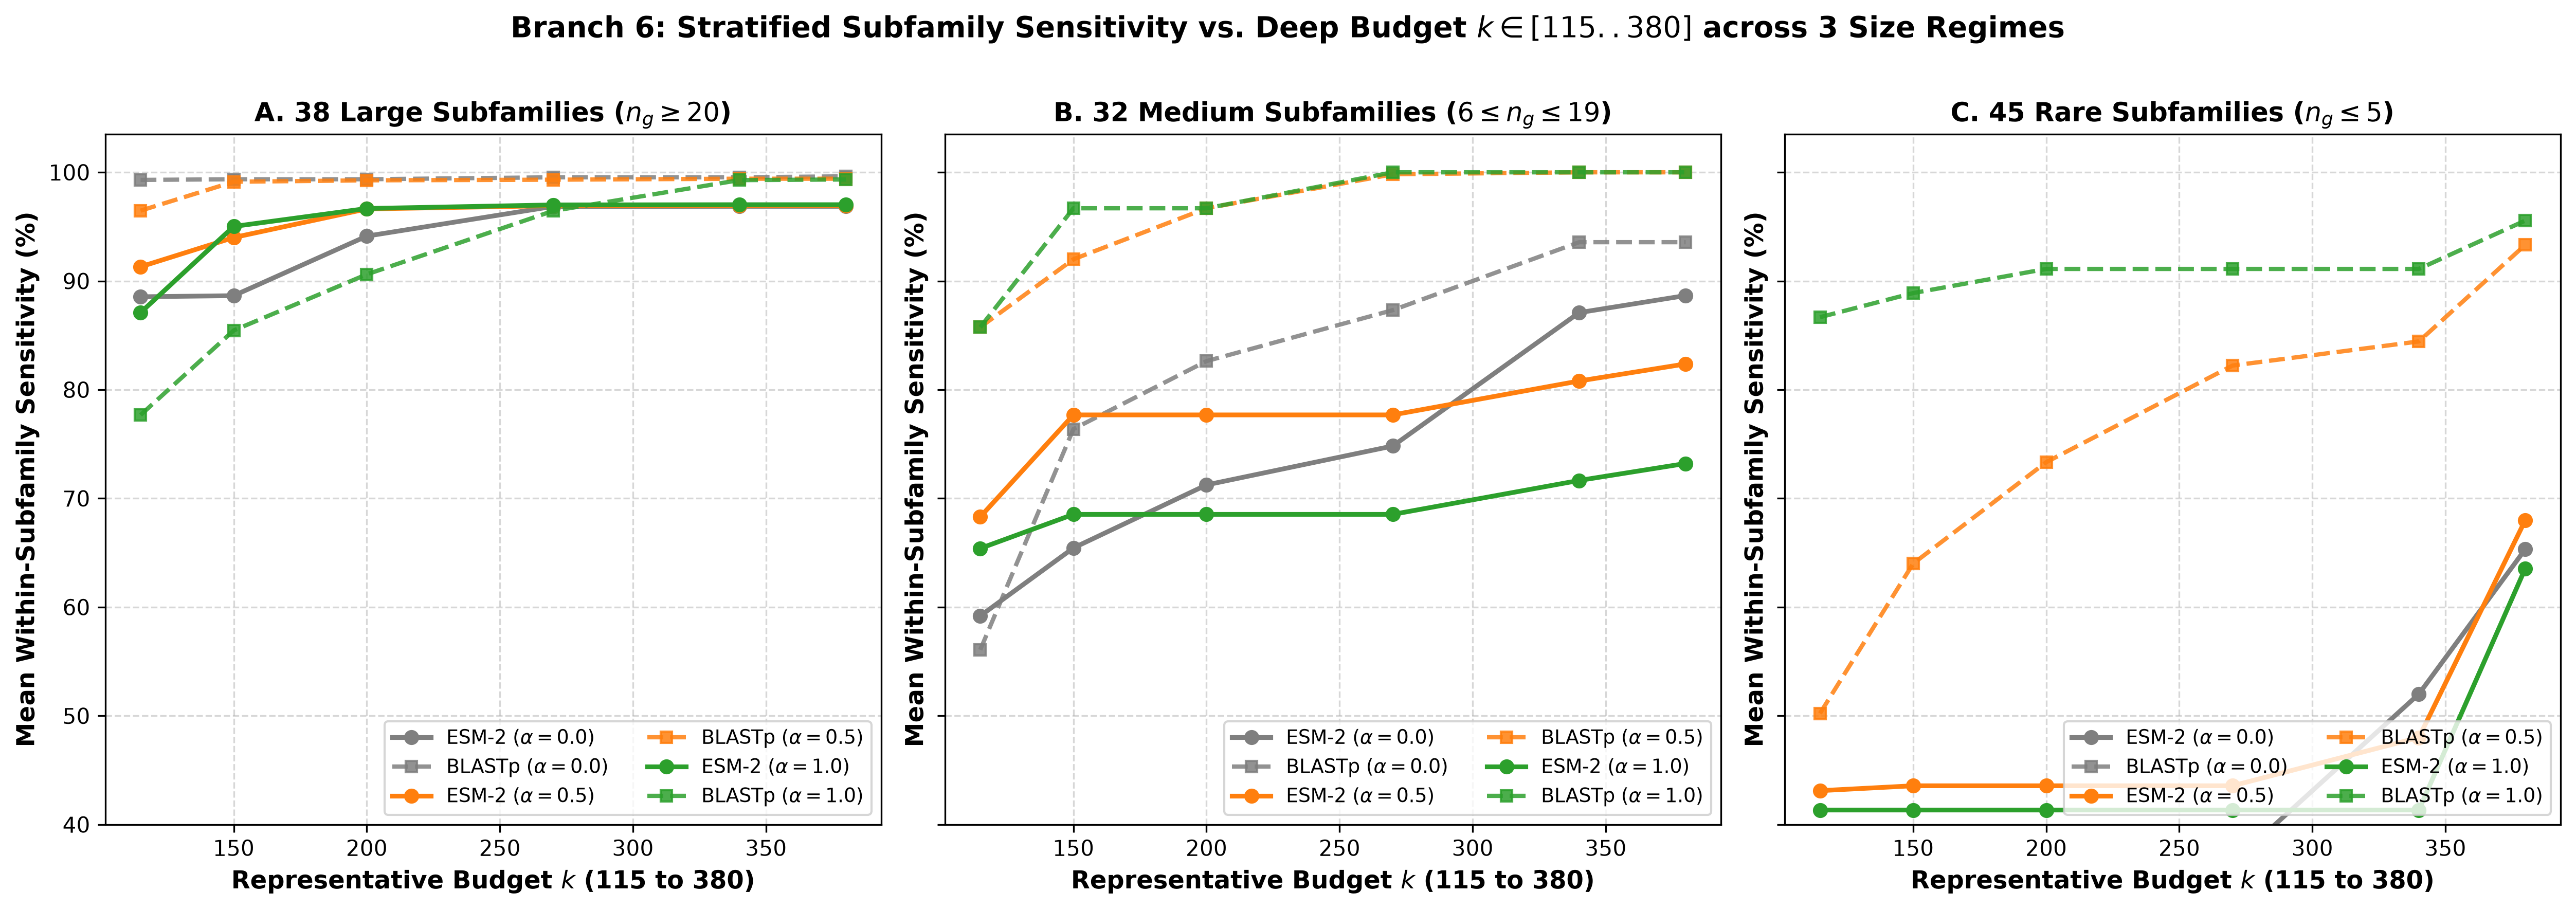
\includegraphics[width=0.92\textwidth]{Images/figures/exp6_stratified_coverage_vs_k.png}
    \caption{Xu hướng biến thiên của chỉ số Sensitivity nội phân họ phân tầng theo ba khối quy mô: lớn, trung bình và hiếm theo quy mô ngân sách mở rộng.}
    \label{fig:exp6_stratified}
\end{figure}

\begin{figure}[htbp!]
    \centering
    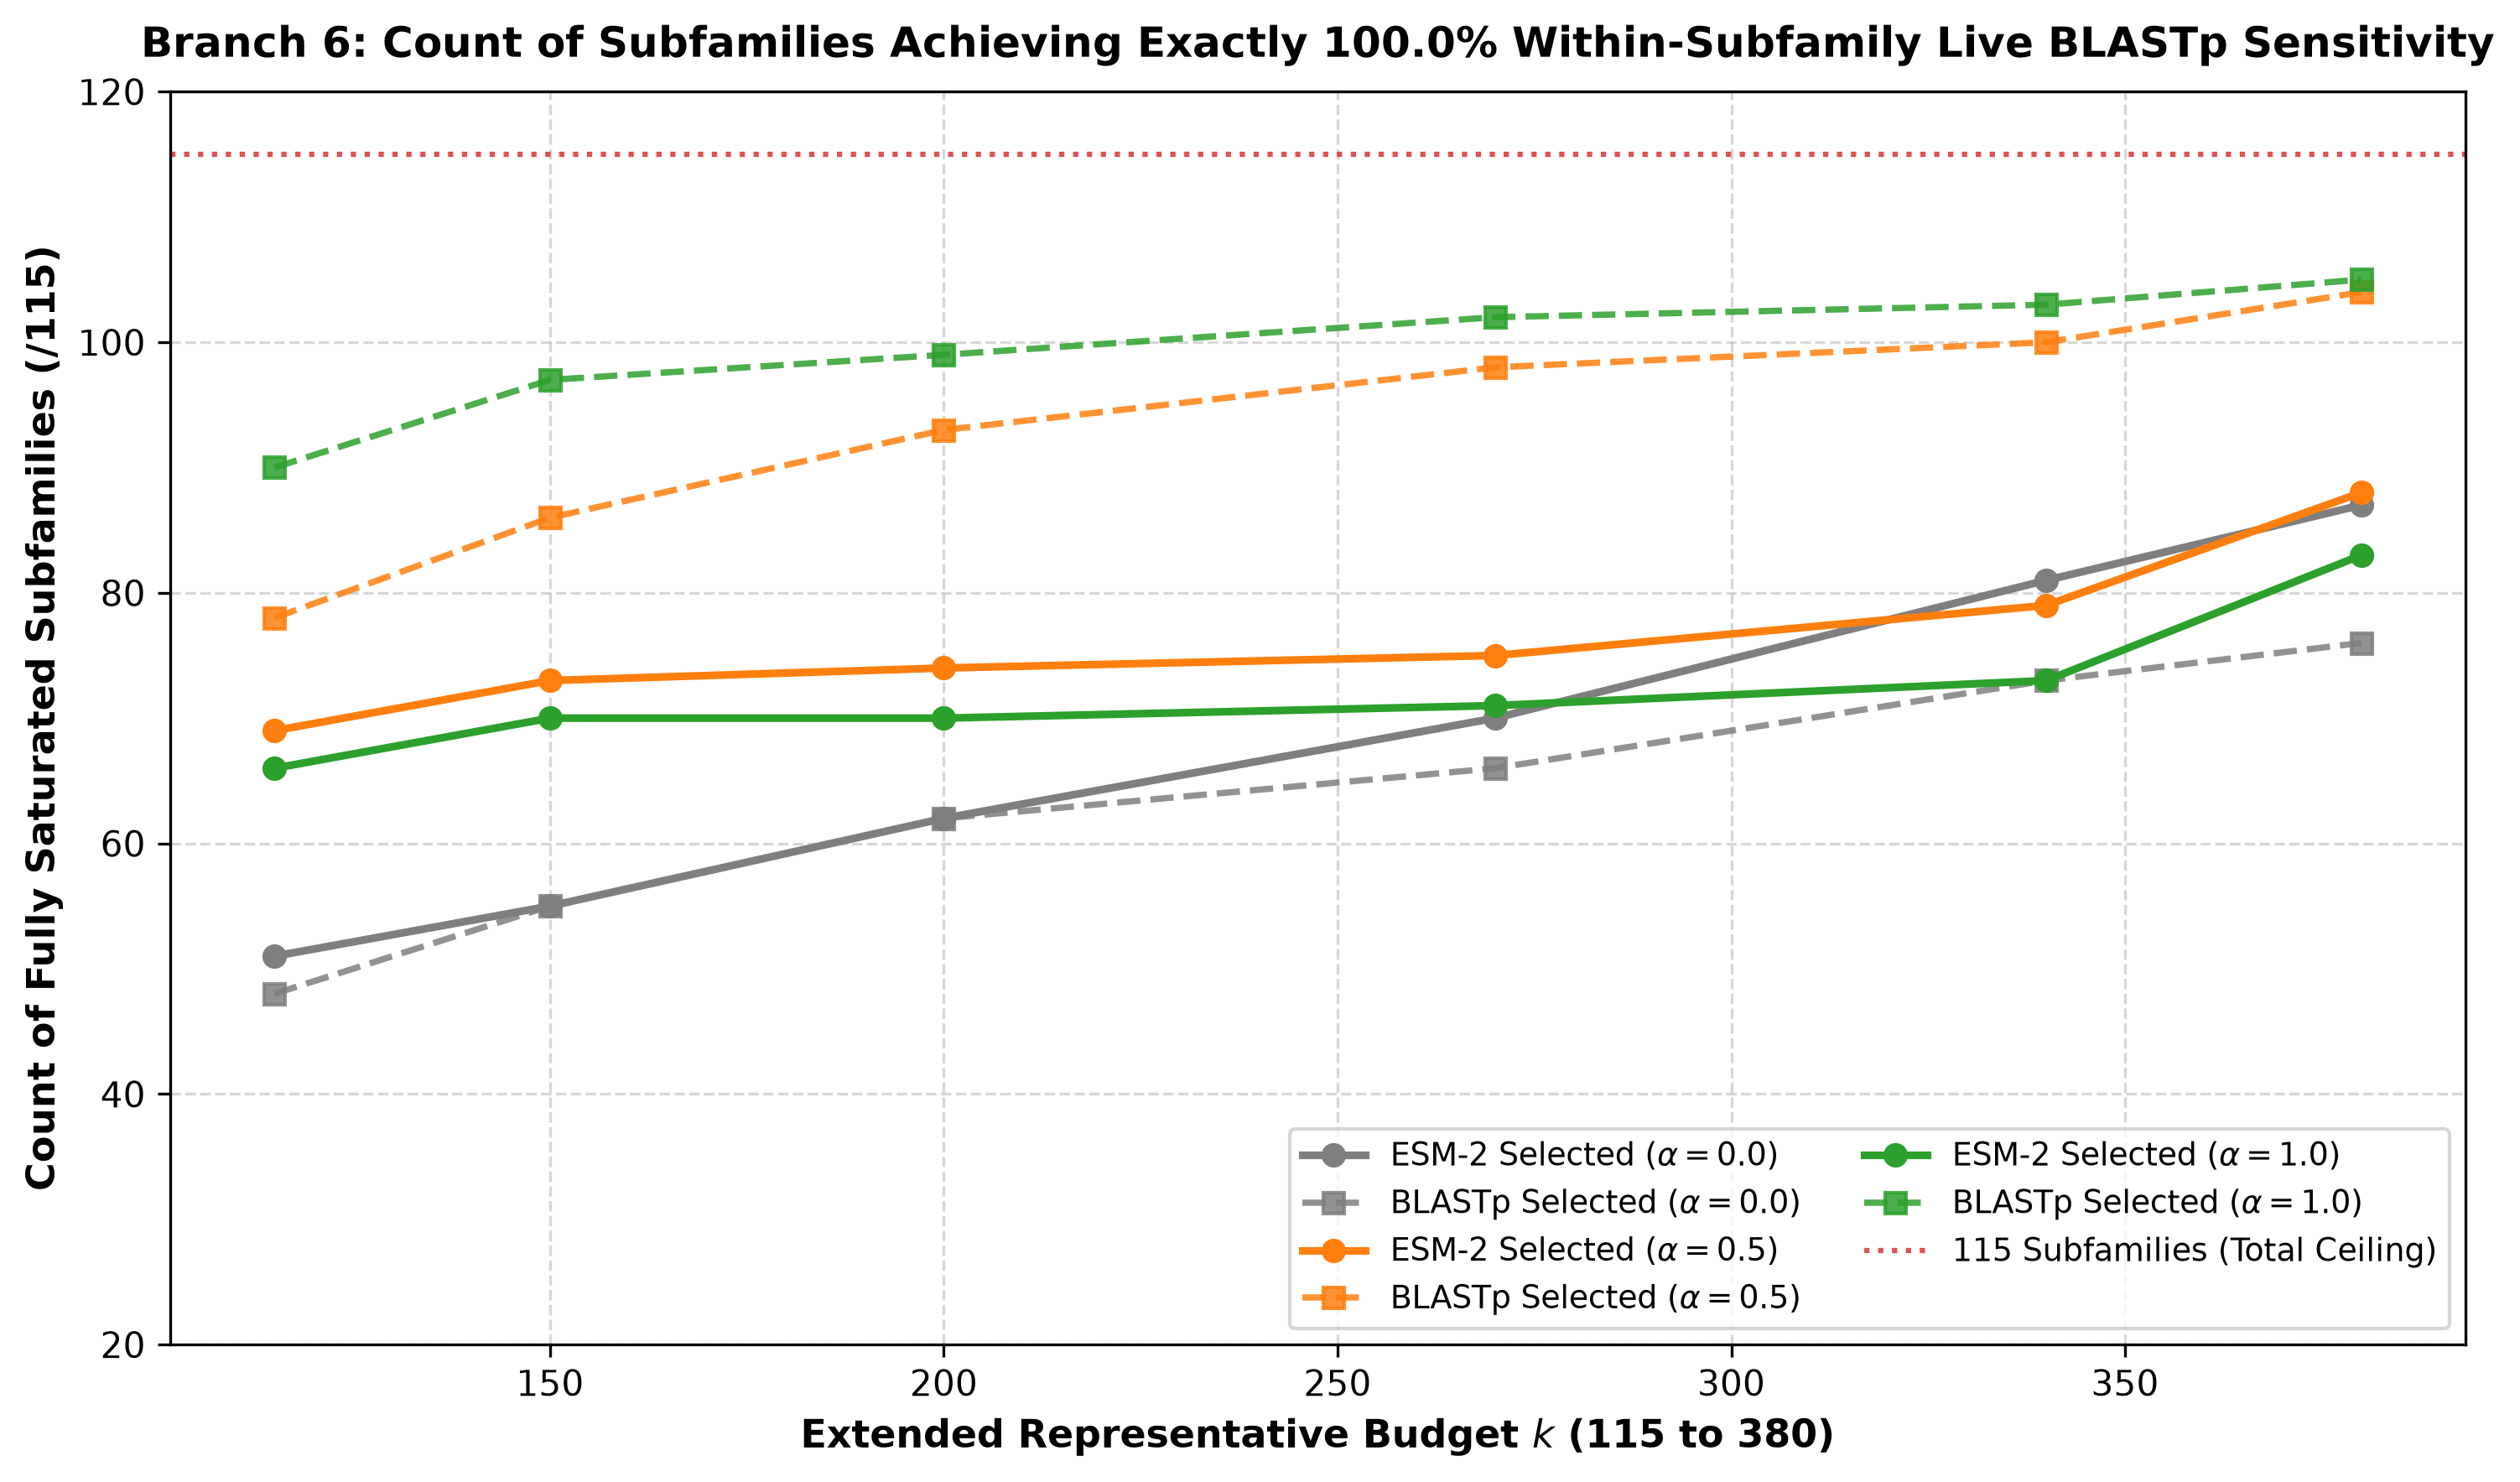
\includegraphics[width=0.82\textwidth]{Images/figures/exp6_full_saturation_count_vs_k.png}
    \caption{Số lượng Subfamily đạt bão hòa 100\% Sensitivity nội phân họ khi mở rộng ngân sách lên $k \in [115..380]$.}
    \label{fig:exp6_saturation}
\end{figure}

\FloatBarrier
\phantomsection\label{sec:exp_discussion}
\phantomsection\label{subsec:rq_resolution_matrix}

Dựa trên dữ liệu thực nghiệm xuyên suốt 6 thử nghiệm, các phát hiện khoa học và bằng chứng định lượng cốt lõi của đề tài được tổng hợp tại bảng~\ref{tab:rq_resolution}.

\begin{table}[htbp!]
\centering
\caption{Tổng hợp các phát hiện thực nghiệm và bằng chứng định lượng cốt lõi của đề tài RareProtSelect.}
\label{tab:rq_resolution}
\vspace{4pt}
\small
\begin{tabularx}{\textwidth}{L{4.2cm}Y}
\toprule
\textbf{Nội dung và thử nghiệm} & \textbf{Kết luận thực nghiệm và bằng chứng khoa học} \\
\midrule
\textbf{Hạn chế bao phủ chéo của mô hình cơ sở} \newline Thử nghiệm 1 và thử nghiệm 2 & Tạo ra sai lệch bao phủ chéo ngoài ranh giới phân họ khi đánh giá toàn cục. Tại $k=1$, chỉ số Overall Sensitivity đạt $82{,}36\%$ nhưng thực chất có tới $114$ trên $115$ Subfamily không có đại diện trực tiếp (Within-Subfamily Overall Sensitivity chỉ đạt $3{,}54\%$). Tại $k=115$, mô hình cơ sở không trọng số vẫn để sót $58$ Subfamily, tương ứng $50{,}43\%$, ở mức $0{,}0\%$ Sensitivity. \\
\addlinespace
\textbf{Tái cân bằng bằng trọng số hiếm trên BLASTp} \newline Thử nghiệm 2 & Đạt hiệu quả cao tại $\alpha = 0{,}5$: Rare Sensitivity tăng gấp $26{,}6$ lần từ $2{,}22\%$ lên $59{,}11\%$, Macro-Average Sensitivity tăng $+29{,}59\%$, khôi phục tính đại diện cho $35$ Subfamily trong khi Overall Sensitivity không giảm, đạt $94{,}13\%$. \\
\addlinespace
\textbf{Mở rộng không gian ngữ nghĩa liên tục ESM-2} \newline Thử nghiệm 3 & Bảo tồn cụm ngữ nghĩa liên tục. Trên ma trận tương đồng đã dịch tâm với $\beta=0{,}70$, trọng số $\alpha=0{,}5$ tăng Rare Coverage ESM gấp $3{,}4$ lần, từ $12{,}85\%$ lên $43{,}21\%$, bắt đầu lựa chọn được đại diện của nhóm hiếm sớm ngay từ mốc $k=8$. \\
\addlinespace
\textbf{Kiểm chứng chéo hai chiều giữa hai không gian} \newline Thử nghiệm 4 & Làm rõ sự đảo chiều về hiệu năng theo ngân sách $k$: ESM-2 đạt kết quả cao hơn gấp từ $1{,}6$ lần đến $4{,}0$ lần ở dải ngân sách từ $k = 8$ đến $k = 75$, trong khi BLASTp đạt kết quả cao hơn tại $k=115$ do tính cô lập phân họ của ma trận thưa. \\
\addlinespace
\textbf{Cơ chế phân bổ vị trí đại diện trong tập nghiệm} \newline Thử nghiệm 5 & Hóa giải sự thiên lệch quy mô mẫu. Tỷ lệ dư thừa giảm từ $50{,}43\%$ xuống $20{,}00\%$, số vị trí đại diện của A01.009 tại $k=115$ được kiểm soát từ $6$ xuống $3$, chiếm $2{,}61\%$ ngân sách, phân bổ đại diện cho $92$ trên $115$ Subfamily và $27$ trên $45$ nhóm hiếm. \\
\addlinespace
\textbf{Hội tụ độ bao phủ khi mở rộng ngân sách} \newline Thử nghiệm 6 & Khi mở rộng ngân sách lên $k = 380$ với $\alpha = 0{,}5$, không gian BLASTp nhận diện chuỗi của $112$ trên $115$ Subfamily ($97{,}39\%$) với $104$ Subfamily đạt $100\%$ Sensitivity; Subfamily lớn nhất A01.009 được tăng cường từ $3$ lên $6$ chuỗi trên BLASTp (nâng Coverage ESM từ $91{,}88\%$ lên $93{,}67\%$) và từ $4$ lên $22$ chuỗi trên ESM-2 (nâng Coverage ESM từ $93{,}27\%$ lên $95{,}81\%$), duy trì $100{,}0\%$ Live BLASTp Sensitivity và chứng minh khả năng vừa bảo toàn nhóm hiếm vừa mở rộng độ bao phủ ngữ nghĩa cho các phân họ lớn có biến dị nội nhóm rộng. \\
\bottomrule
\end{tabularx}
\end{table}

Bảng~\ref{tab:rq_resolution} tổng hợp các phát hiện thực nghiệm chính, làm rõ ba đóng góp phương pháp luận của đề tài: thứ nhất, làm rõ cơ chế sai lệch bao phủ chéo ngoài ranh giới phân họ của mô hình không trọng số; thứ hai, thiết lập cấu hình trọng số cân bằng với mức tăng trưởng gấp $26{,}6$ lần về chỉ số Rare Sensitivity trên không gian BLASTp và gấp $3{,}4$ lần trên không gian ESM-2; và thứ ba, xác lập quy luật phân bổ đại diện công bằng, giảm độ dư thừa từ $50{,}43\%$ xuống $20{,}00\%$ và chuyển dịch vị trí đại diện sang các Subfamily hiếm.

\phantomsection\label{subsec:method_comparison}

So với các công cụ gom cụm và chọn đại diện truyền thống như CD-HIT~\cite{cdhit} hay MMseqs2~\cite{mmseqs2}, RareProtSelect thể hiện ba ưu điểm về phương pháp luận: thứ nhất, khả năng kiểm soát trực tiếp lực lượng tập đại diện theo bài toán ràng buộc ngân sách $|S| \le k$ thay vì phụ thuộc vào việc dò tìm ngưỡng tương đồng cứng dựa trên phương pháp heuristic; thứ hai, bảo đảm toán học giải tích chặt chẽ qua cận xấp xỉ Nemhauser $(1 - 1/e) \approx 63{,}2\%$ giá trị tối ưu toàn cục mà các thuật toán gom cụm heuristic không thể cung cấp; và thứ ba, cơ chế tái cân bằng trọng số linh hoạt qua tham số $\alpha$, cho phép người dùng chủ động điều tiết mức độ ưu tiên bảo tồn nhóm hiếm và tối ưu hóa hiệu quả đánh đổi đa mục tiêu trên các phân bố sinh học mất cân bằng lớn về quy mô. Kết quả thực nghiệm khẳng định tính hiệu quả của khung phương pháp đề xuất.

\chapter{Kết luận và hướng phát triển}
\label{chap:conclusion}

Đồ án đã hoàn thành mục tiêu nghiên cứu về bài toán chọn tập chuỗi protein đại diện có ưu tiên nhóm hiếm thông qua mô hình tối ưu hóa submodular có trọng số. Từ việc chỉ ra hạn chế phương pháp luận của hàm mục tiêu không trọng số truyền thống tại chương~\ref{chap:theory}, thiết lập khung phương pháp luận RareProtSelect và chứng minh chặt chẽ các bảo đảm toán học tại chương~\ref{chap:methodology}, đến việc thực thi chuỗi 6 thử nghiệm tuần tự có kiểm soát tại chương~\ref{chap:experiments}, đồ án đã khẳng định tính đúng đắn cả về mặt lý thuyết giải tích lẫn thực nghiệm tính toán sinh học. Chương~\ref{chap:conclusion} hệ thống hóa các kết quả và đóng góp khoa học chính, làm rõ ranh giới kiểm chứng cùng các hạn chế nội tại, đồng thời mở ra các định hướng nghiên cứu tiếp theo nhằm hoàn thiện và mở rộng khung phương pháp.

\section{Tổng kết đóng góp khoa học và kết luận định hướng ứng dụng}
\label{sec:conc_contributions}

Thay vì liệt kê lặp lại số liệu của từng thử nghiệm riêng lẻ đã được tổng hợp tại bảng~\ref{tab:rq_resolution}, phần này đúc kết các phát hiện khoa học ở cấp độ phương pháp luận: đánh giá bản chất vì sao khung phương pháp đề xuất thực sự hiệu quả, làm sáng tỏ vai trò củng cố của các khảo sát mở rộng đa chiều, và xác lập hướng dẫn lựa chọn cấu hình cụ thể cho từng tình huống sinh học thực tế.

\subsection{Đánh giá tính hiệu quả của phương pháp đề xuất và cơ chế giải quyết đánh đổi đa mục tiêu}
\label{subsec:conc_core_effectiveness}
\phantomsection\label{subsec:conc_five_tasks}
\phantomsection\label{subsec:conc_core_methodology}

Đồ án đã giải quyết đầy đủ năm nhiệm vụ nghiên cứu đặt ra tại phần Mở đầu: từ việc sàng lọc và thiết lập tập dữ liệu phân họ chính thức $V_{\text{curated}}$ gồm $4.120$ chuỗi thuộc $115$ Subfamily từ $13.847$ chuỗi thô của tệp MEROPS\_A1A.fasta~\cite{merops} tại mục~\ref{subsec:methodology_curation}; tái lập độc lập mô hình cơ sở của Nguyen và cộng sự~\cite{nguyen2025} trên $13.307$ chuỗi với sai số tuyệt đối trung bình chỉ $0{,}51\%$ tại bảng~\ref{tab:exp1_milestones} và vạch rõ sai lệch bao phủ chéo ngoài ranh giới phân họ; thiết kế họ hàm mục tiêu Weighted Facility Location $F_\alpha(S)$ tại công thức~\eqref{eq:sample_weight_formula}--\eqref{eq:weighted_facility_location}, chứng minh tính đơn điệu không giảm tại bổ đề~\ref{lem:monotonicity}, tính submodular tại định lý~\ref{thm:submodularity}, thiết lập nền tảng lý thuyết theo cận xấp xỉ Nemhauser $(1 - 1/e) \approx 63{,}2\%$ của giải thuật tham lam chuẩn tại hệ quả~\ref{cor:nemhauser_guarantee}~\cite{nemhauser1978} làm cơ sở cho giải thuật thực thi Pruned Greedy 90\% trên GPU tại thuật toán~\ref{alg:gpu_pruned_greedy}; đến việc khảo sát không gian ngữ nghĩa ESM-2~\cite{esm2} kết hợp dịch tâm Mean-Centering với $\beta = 0{,}70$ tại thuật toán~\ref{alg:mean_centering}; và hoàn tất kiểm chứng chéo hai chiều, phân tích phân bổ vi mô cùng khảo sát mở rộng ngân sách. Từ toàn bộ chuỗi nghiên cứu này, kết luận cốt lõi được khẳng định là phương pháp đề xuất RareProtSelect mang lại hiệu quả thực chất nhờ giải quyết đồng thời hai mục tiêu: vừa khôi phục khả năng nhận diện các Subfamily hiếm, vừa duy trì độ bao phủ toàn cục, thay vì phải đánh đổi hay hy sinh hiệu năng tổng thể như các cách tiếp cận thông thường.

Trong các nghiên cứu chọn tập đại diện truyền thống, việc gia tăng tính đại diện cho các nhóm hiếm thường bị mặc định là mục tiêu đối nghịch trực tiếp với việc tối đa hóa độ bao phủ toàn cục. Đồ án đã chỉ ra rằng tại mốc ngân sách đủ lớn trên các siêu họ protein có phân bố đuôi dài với tỷ lệ chênh lệch quy mô gấp $329{,}0$ lần theo công thức~\eqref{eq:imbalance_ratio}, hai mục tiêu này có thể đồng thời đạt được. Khi áp dụng thước đo nội phân họ Within-Subfamily Coverage theo công thức~\eqref{eq:within_subfamily_reps}--\eqref{eq:within_subfamily_covered_set}, mô hình không trọng số ($\alpha = 0{,}0$) tại ngân sách chuẩn $k = 115$ bộc lộ sự lãng phí ngân sách đại diện: giải thuật dồn tới $58$ vị trí đại diện trùng lặp vào các Subfamily lớn đã bão hòa độ bao phủ nội bộ, trong khi bỏ sót $58$ trên $115$ Subfamily, chiếm $50{,}43\%$, ở mức $0{,}0\%$ Sensitivity. Bằng cách điều chỉnh tổng trọng số của mỗi phân họ theo hàm lũy thừa $W_g^{(\alpha)} = (n_g)^{1-\alpha}$ tại công thức~\eqref{eq:subfamily_total_weight}, cấu hình trọng số cân bằng $\alpha = 0{,}5$ thu hẹp tỷ lệ chênh lệch đóng góp giữa Subfamily lớn nhất A01.009 và Subfamily đơn độc từ $329{,}0$ lần xuống $18{,}14$ lần. Cơ chế này không làm mất đi các chuỗi đại diện thiết yếu của các Subfamily lớn, mà chỉ hạn chế các lượt chọn trùng lặp có độ tăng cận biên thấp ở nhóm lớn để chuyển dịch ngân sách sang các phân họ chưa có đại diện. Cần nhấn mạnh rằng sự giải tỏa đánh đổi đa mục tiêu này đạt được tại mốc ngân sách đủ lớn $k = G = 115$ với cấu hình cân bằng $\alpha = 0{,}5$, nơi các Subfamily lớn đã đạt bão hòa nội nhóm; trong khi ở các mức ngân sách nhỏ và vừa ($k < G$), việc bảo tồn nhóm hiếm vẫn đòi hỏi sự đánh đổi một phần chỉ số Overall Sensitivity, chẳng hạn tại $k = 30$, cấu hình $\alpha = 0{,}5$ đạt $4{,}44\%$ Rare Sensitivity nhưng chỉ số Overall Sensitivity giảm $8{,}93$ điểm phần trăm từ $71{,}65\%$ xuống $62{,}72\%$ so với $\alpha = 0{,}0$. Tại $k = 115$, trên không gian NCBI BLASTp~\cite{blast}, cấu hình $\alpha = 0{,}5$ nâng chỉ số Rare Sensitivity từ $2{,}22\%$ lên $59{,}11\%$, tức tăng gấp $26{,}6$ lần khi cố định ngưỡng ngân sách tối đa $k_{\max} = 115$, và đạt $50{,}22\%$, tức tăng gấp $22{,}6$ lần khi ngưỡng ngân sách tối đa mở rộng lên $k_{\max} = 380$; đồng thời chỉ số Macro-Average Sensitivity tăng từ $49{,}28\%$ lên $78{,}87\%$ trong khi chỉ số Overall Sensitivity đạt $94{,}13\%$ so với $93{,}57\%$ của mô hình cơ sở. Đây là bằng chứng thực nghiệm khẳng định tính hiệu quả có điều kiện biên của phương pháp đề xuất.

\subsection{Giá trị củng cố luận điểm khoa học từ các khảo sát mở rộng đa chiều}
\label{subsec:conc_reinforcing_surveys}
\phantomsection\label{subsec:conc_exploratory_esm2}

Bên cạnh kết quả trọng tâm trên không gian tương đồng chuỗi BLASTp ở ngân sách cơ sở, bốn thử nghiệm mở rộng từ thử nghiệm 3 đến thử nghiệm 6 tại chương~\ref{chap:experiments} hợp thành ba tầng bằng chứng độc lập làm rõ tính nhất quán, tính tường minh của cơ chế tối ưu hóa và khả năng mở rộng quy mô của phương pháp đề xuất:

\begin{enumerate}
    \item \textbf{Củng cố tính tổng quát không phụ thuộc không gian biểu diễn và quy luật tương tác cấu trúc ma trận:} Việc tích hợp module khảo sát mở rộng ESM-2 kết hợp kỹ thuật dịch tâm Mean-Centering với $\beta = 0{,}70$ tại thử nghiệm 3 và bảng~\ref{tab:exp3_milestones} chứng minh công thức trọng số nghịch đảo quy mô không bị phụ thuộc cục bộ vào đặc thù ma trận thưa BLASTp. Ngay trên không gian hình học liên tục có cấu trúc đặc với $99{,}64\%$ phần tử dương sau khi dịch tâm, trọng số $\alpha = 0{,}5$ vẫn nhất quán nâng chỉ số Rare Coverage ESM tăng gấp $3{,}4$ lần, từ $12{,}85\%$ lên $43{,}21\%$. Đặc biệt, ma trận kiểm chứng chéo hai chiều $2 \times 2$ trên $120$ cấu hình tại thử nghiệm 4 và bảng~\ref{tab:exp4_cross_milestones} đã củng cố hiểu biết lý thuyết về quy luật tương tác giữa cấu trúc ma trận và quy mô ngân sách $k$: ma trận đặc ESM-2 phát huy ưu thế dẫn truyền thông tin ngữ nghĩa liên cụm khi ngân sách hẹp ($k \in [8..75]$), giúp nhận diện sớm nhóm hiếm ngay từ $k = 8$ và đạt hiệu năng cao hơn gấp $1{,}6$ đến $4{,}0$ lần so với BLASTp; ngược lại, tính cô lập phân họ của ma trận thưa BLASTp giúp duy trì độ tăng cận biên cho các phân họ hiếm còn sót lại khi ngân sách đủ lớn ($k = 115$), đạt tỷ lệ bao phủ $92$ trên $115$ Subfamily so với $77$ trên $115$ của ESM-2.
    
    \item \textbf{Làm sáng tỏ cơ chế phân bổ đại diện bên trong quá trình tối ưu hóa qua phân tích vi mô:} Khảo sát cấu trúc nhãn phân họ trực tiếp của từng chuỗi trong tập nghiệm $S_k$ tại thử nghiệm 5 và bảng~\ref{tab:exp5_milestones} cung cấp bằng chứng nhân quả giải thích trực tiếp kết quả của thử nghiệm 2 và thử nghiệm 3. Số liệu chứng minh sự cải thiện tỷ lệ nhận diện chuỗi không bắt nguồn từ nhiễu ngẫu nhiên, mà do trọng số $\alpha = 0{,}5$ đã cắt giảm độ dư thừa phân bổ Subfamily Redundancy từ $50{,}43\%$ xuống $20{,}00\%$, qua đó chuyển dịch đúng $35$ vị trí đại diện từng bị phân bổ trùng lặp ở các nhóm lớn, điển hình là giảm một nửa tỷ trọng của Subfamily lớn nhất A01.009 tại mốc chuẩn $k = 115$ từ $6$ vị trí ($5{,}22\%$) ở $\alpha = 0{,}0$ xuống còn $3$ vị trí ($2{,}61\%$) ở $\alpha = 0{,}5$ (và tương tự tại $k = 11$ giảm từ $18{,}18\%$ xuống $9{,}09\%$), sang cho $35$ Subfamily chưa có đại diện. Điều này giúp nâng số lượng phân họ hiếm có đại diện từ $1$ lên $27$ trên $45$ Subfamily, đạt $60{,}00\%$ ở $\alpha = 0{,}5$ và đạt $41$ trên $45$ Subfamily, tức $91{,}11\%$ ở $\alpha = 1{,}0$.
    
    \item \textbf{Củng cố năng lực bao phủ đồng thời nhóm hiếm và biến dị nội nhóm của các phân họ lớn khi mở rộng ngân sách:} Thực nghiệm mở rộng ngân sách theo cấu trúc phân tầng lên $k = 380$ tại thử nghiệm 6 và bảng~\ref{tab:exp6_milestones} giải đáp câu hỏi về việc giảm số đại diện của Subfamily lớn nhất A01.009 xuống $3$ chuỗi tại $k = 115$ liệu có làm mất thông tin biến dị nội nhóm của phân họ có quy mô lớn nhất này hay không. Phân họ A01.009 vốn đã đạt $100{,}0\%$ Sensitivity nội phân họ ngay tại $k = 115$; khi ngân sách được nới rộng lên $k = 380$, hàm mục tiêu $\alpha = 0{,}5$ không chỉ nâng độ bao phủ lên $112$ trên $115$ Subfamily, đạt $97{,}39\%$, với $104$ Subfamily đạt bão hòa $100\%$ Sensitivity, mà còn tự động phân bổ bổ sung thành $6$ chuỗi đại diện cho A01.009 trên không gian BLASTp (nâng Coverage ESM từ $91{,}88\%$ lên $93{,}67\%$) và $22$ chuỗi trên không gian ESM-2 (nâng Coverage ESM từ $93{,}27\%$ lên $95{,}81\%$), nâng cao độ bao phủ biến dị ngữ nghĩa liên tục cho phân họ lớn này.
\end{enumerate}

\subsection{Khuyến nghị lựa chọn cấu hình theo tình huống thực tế}
\label{subsec:conc_config_guidelines}

Từ các bằng chứng thực nghiệm và phân tích cơ chế trên cả hai không gian biểu diễn, đồ án xác lập bộ khuyến nghị lựa chọn cấu hình RareProtSelect cho bốn tình huống ứng dụng sinh học:

\begin{enumerate}
    \item \textbf{Tình huống 1: Chọn tập đại diện chuẩn đa mục tiêu ở ngân sách cơ sở tương đương số lượng phân họ ($k \approx G$).} Khuyến nghị sử dụng không gian tương đồng chuỗi NCBI BLASTp kết hợp hệ số trọng số cân bằng $\alpha = 0{,}5$ tại ngân sách $k = G$, tương ứng $k = 115$ trên Family A1. Đây là cấu hình mặc định tối ưu cho đại đa số các bài toán tiền xử lý so khớp đa chuỗi, dựng cây phát sinh chủng loài toàn siêu họ và xây dựng tập dữ liệu huấn luyện cân bằng. Ở cấu hình này, người dùng đạt được trạng thái cân bằng đa mục tiêu tối ưu: duy trì chỉ số Overall Sensitivity ở mức cao đạt $94{,}13\%$, khôi phục đáng kể tỷ lệ nhận diện phân họ hiếm đạt $59{,}11\%$, gấp $26{,}6$ lần mô hình cơ sở, đại diện cho $80{,}00\%$ tổng số Subfamily và giảm thiểu độ dư thừa xuống chỉ còn $20{,}00\%$.
    
    \item \textbf{Tình huống 2: Sàng lọc nhanh với ngân sách siêu tinh gọn ($k \ll G$) hoặc khảo sát các họ protein phân kỳ tiến hóa xa.} Khuyến nghị sử dụng không gian ngữ nghĩa liên tục ESM-2 kết hợp dịch tâm Mean-Centering với $\beta = 0{,}70$ và trọng số $\alpha = 0{,}5$ ở dải ngân sách hẹp $k \in [8..75]$. Cấu hình này phù hợp cho các bước phân tích sinh học tiếp theo có chi phí tính toán hoặc chi phí thực nghiệm cao trên mỗi chuỗi, chẳng hạn như mô phỏng động lực học phân tử, sàng lọc tương tác thuốc trên cấu trúc không gian ba chiều hoặc tổng hợp protein thực nghiệm trong phòng thí nghiệm, nơi số lượng chuỗi đại diện được phép chọn nhỏ hơn nhiều so với tổng số phân họ. Khi đó, khả năng nắm bắt tương đồng cấu trúc tầm xa của ma trận đặc ESM-2 giúp tập đại diện siêu nhỏ vẫn nhận diện sớm các nhóm hiếm ngay từ $k = 8$ và đạt hiệu năng bảo tồn nhóm hiếm cao hơn gấp $1{,}6$ đến $4{,}0$ lần so với sử dụng BLASTp cùng mức trọng số $\alpha = 0{,}5$. Tuy nhiên, nếu mục tiêu thực nghiệm tại $k = 60$ là tối đa hóa trực tiếp tỷ lệ nhận diện Live BLASTp Sensitivity, việc sử dụng BLASTp với trọng số mạnh $\alpha = 1{,}0$ đạt kết quả cao hơn rõ rệt, với $57{,}04\%$ Rare Sensitivity so với $28{,}89\%$ của ESM-2 $\alpha = 0{,}5$ và $40{,}44\%$ của ESM-2 $\alpha = 1{,}0$, trong khi vẫn duy trì chỉ số Overall Sensitivity ở mức $62{,}57\%$.
    
    \item \textbf{Tình huống 3: Nghiên cứu chuyên sâu về tiến hóa nhóm hiếm và bảo tồn tối đa các nhánh đơn độc.} Khuyến nghị sử dụng không gian tương đồng chuỗi NCBI BLASTp kết hợp hệ số trọng số bình đẳng nhóm $\alpha = 1{,}0$ tại ngân sách $k \ge G$. Cấu hình này phù hợp cho các nghiên cứu sinh học tiến hóa chuyên sâu nhằm lập bản đồ các nhánh phân loại hiếm, tìm kiếm các enzyme có cơ chế xúc tác đặc hữu hoặc bảo vệ các Subfamily đơn độc chỉ có duy nhất $1$ chuỗi trong cơ sở dữ liệu. Nhờ thiết lập tổng trọng số của mọi phân họ ngang nhau ($W_g^{(1{,}0)} = 1$), cấu hình này đẩy chỉ số Rare Sensitivity lên mức cao nhất $91{,}11\%$, bảo tồn $41$ trên $45$ Subfamily hiếm, tăng gấp $41{,}0$ lần so với mô hình không trọng số, phù hợp khi người nghiên cứu ưu tiên cao nhất độ bao phủ phân loại và chấp nhận giảm mật độ lấy mẫu ở các phân họ phổ biến, với Overall Sensitivity ở mức $79{,}08\%$.
    
    \item \textbf{Tình huống 4: Xây dựng thư viện tham chiếu đầy đủ cho các siêu họ có biến dị nội nhóm lớn.} Khuyến nghị sử dụng không gian tương đồng chuỗi NCBI BLASTp kết hợp hệ số trọng số cân bằng $\alpha = 0{,}5$ và mở rộng ngân sách theo cấu trúc phân tầng lên $k \approx 2{,}5G \text{ đến } 3{,}3G$, tương ứng $k \in [270..380]$ trên Family A1. Cấu hình này được khuyến nghị khi xây dựng bộ dữ liệu chuỗi đại diện tham chiếu hoặc bộ khung phân loại cho toàn siêu họ, nơi đòi hỏi cả hai mục tiêu đều phải tiệm cận mức bão hòa: vừa bao phủ $97{,}39\%$ tổng số phân họ, tức $112$ trên $115$ Subfamily, và đạt $93{,}33\%$ Rare Sensitivity, vừa phân bổ đủ từ $5$ đến $6$ chuỗi đại diện cho các phân họ quy mô lớn có biến dị nội nhóm rộng như A01.009 để duy trì $100{,}0\%$ Sensitivity và nâng Coverage ESM lên $93{,}67\%$, đồng thời giúp $104$ trên $115$ Subfamily đạt bão hòa $100\%$ Sensitivity.
\end{enumerate}

\section{Ranh giới kiểm chứng và các hạn chế tồn tại}
\label{sec:conc_limitations}

Bên cạnh những kết quả đạt được, việc xác định rõ phạm vi kiểm chứng thực nghiệm và các giới hạn nội tại của mô hình là cơ sở cần thiết để ứng dụng phương pháp một cách phù hợp và định hướng cải tiến trong tương lai. Qua quá trình thực nghiệm trên siêu họ Peptidase Family A1, khung phương pháp luận RareProtSelect còn tồn tại ba nhóm hạn chế phương pháp luận cần được phân tích làm rõ.

\subsection{Sự phụ thuộc vào nhãn phân họ có sẵn, sự gắn kết nhãn của thước đo và phạm vi các phương pháp đối chứng cố định ngân sách}
\label{subsec:lim_unassigned_upa}

Hạn chế căn bản đầu tiên nằm ở sự phụ thuộc vào hệ thống nhãn phân loại có sẵn. Công thức trọng số nghịch đảo quy mô $w_v^{(\alpha)} = (n_{g(v)})^{-\alpha}$ được xây dựng dựa trên tiền đề mỗi chuỗi protein $v \in V$ đều đã có nhãn phân họ xác định $g(v) \in \{1, \dots, G\}$. 

Đối với cơ sở dữ liệu MEROPS, tệp MEROPS\_A1A.fasta chứa tới $9.187$ chuỗi mang nhãn [A01.UPA], chiếm $69{,}04\%$ tổng số chuỗi đã qua kiểm soát chất lượng. Việc sàng lọc loại bỏ khối [A01.UPA] để xây dựng tập dữ liệu phân họ chính thức $V_{\text{curated}}$ gồm $4.120$ chuỗi là giải pháp bắt buộc nhằm bảo đảm tính chính xác cho phép đo nội phân họ. Tuy nhiên, điều này giới hạn phạm vi kiểm chứng hiện tại trong không gian các chuỗi đã có định danh phân loại, chưa thể trực tiếp xử lý các tập dữ liệu metagenomics môi trường chứa nhiều chuỗi chưa phân loại.

Đồng thời, việc cả trọng số tối ưu hóa $w_v^{(\alpha)}$ lẫn cơ chế đánh giá Within-Subfamily Coverage ($S_k \cap V_g \to V_g$) đều dựa trên cùng một hệ thống phân hoạch Subfamily tạo ra một sự tương thích có giám sát giữa mục tiêu huấn luyện và thước đo đánh giá. Khi so sánh với mô hình không trọng số ($\alpha = 0{,}0$) vốn không sử dụng thông tin nhãn, cấu hình $\alpha > 0$ hiển nhiên nắm giữ lợi thế về mặt thông tin cấu trúc. Hơn nữa, nếu nhãn phân họ đã biết trước tại đúng mốc ngân sách $k = G = 115$, một phương pháp đối chứng hạn mức cứng đơn giản là 1-medoid-per-subfamily có thể đạt $100\%$ Subfamily Representation và $100\%$ Rare Representation, cao hơn mức $80{,}00\%$ của $\alpha = 0{,}5$ và $84{,}35\%$ của $\alpha = 1{,}0$. Dù chiến lược 1-medoid-per-subfamily không giải quyết được bài toán xếp hạng liên tục ở $k \ll G$ hay phân bổ đa đại diện theo độ phân kỳ nội họ ở $k > G$, việc chưa triển khai thực nghiệm đối chứng trực tiếp với các phương pháp cố định ngân sách $k$ như chọn ngẫu nhiên, 1-medoid-per-subfamily hoặc CD-HIT/MMseqs2 tinh chỉnh nhị phân ngưỡng tương đồng là một giới hạn phạm vi thực nghiệm cần được bổ sung.

\subsection{Khoảng cách giữa cận xấp xỉ lý thuyết và giải thuật heuristic thực nghiệm, ảnh hưởng của ngưỡng ngân sách tối đa và phương sai xáo trộn}
\label{subsec:lim_static_hyperparams}

Hạn chế thứ hai liên quan đến khoảng cách giữa bảo chứng toán học lý thuyết và giải thuật thực thi trong thực nghiệm. Cận xấp xỉ lý thuyết $(1 - 1/e) \approx 63{,}2\%$ của định lý Nemhauser~\cite{nemhauser1978} áp dụng chặt chẽ cho giải thuật Standard Greedy tối ưu hóa hàm mục tiêu nội tại $F_\alpha(S)$. Để giảm chi phí tính toán trên tập dữ liệu lớn, quy trình thực nghiệm sử dụng cơ chế cắt tỉa cứng $\theta = 0{,}90$ kết hợp lấy top-$k$ theo tần suất đồng thuận qua $1.000$ vòng xáo trộn và đánh giá bằng công cụ Live BLASTp độc lập ($E \le 10^{-7}$). Đây là một giải thuật xấp xỉ heuristic thực nghiệm, không kế thừa nguyên vẹn cận bảo đảm xấu nhất $(1 - 1/e)$. Ngoài ra, ma trận $\mathbf{S}_{\text{BLAST}} = \text{pident}/100$ kế thừa từ bài báo gốc chưa tích hợp tỷ lệ bao phủ chiều dài so khớp (qcovs), khiến hai protein chỉ tương đồng ở một motif xúc tác ngắn vẫn có thể kích hoạt điều kiện cắt tỉa.

Bên cạnh đó, việc trích xuất tập đại diện $S_k$ thông qua tiêu chí sắp xếp tần suất $C(v)$ trên toàn bộ $k_{\max}$ bước khiến danh sách đại diện phụ thuộc vào ngưỡng ngân sách tối đa $k_{\max}$ của từng vòng xáo trộn: tại lát cắt $k = 115$, việc mở rộng $k_{\max}$ từ $115$ lên $380$ làm thay đổi thứ hạng đồng thuận và giảm nhẹ chỉ số Rare Sensitivity từ $59{,}11\%$ xuống $50{,}22\%$. Cuối cùng, toàn bộ kết quả đo đạc trong nghiên cứu hiện được báo cáo trên một danh sách đồng thuận duy nhất khởi tạo từ $\text{seed} = 42$ mà chưa xuất độ lệch chuẩn hay khoảng tin cậy ($\text{mean} \pm \text{std}$) qua nhiều lượt chạy xáo trộn độc lập, đòi hỏi sự cẩn trọng khi diễn giải độ ổn định của các con số thống kê.

\subsection{Hiện tượng bão hòa ma trận tương đồng đặc trên ESM-2, đặc tính bậc thang của thước đo và phạm vi kiểm chứng trên một siêu họ}
\label{subsec:lim_dense_matrix_saturation}

Hạn chế thứ ba xuất phát từ bản chất toán học của ma trận tương đồng đặc trong không gian biểu diễn vector nhúng ESM-2. Kỹ thuật dịch tâm Mean-Centering với $\beta = 0{,}70$ giúp kéo giãn phân bố khoảng cách, song ma trận $\mathbf{S}_{\text{ESM}}^{(\beta=0{,}70)}$ vẫn duy trì tính chất đặc với $99{,}64\%$ phần tử dương.

Khi giải thuật tham lam vận hành ở vùng ngân sách mở rộng ($k \ge 115$), tập nghiệm $S_k$ tích lũy nhiều chuỗi đại diện khiến giá trị bao phủ nền $m_v^{(t)} = \max_{s \in S_t} \mathbf{S}_{\text{ESM}}(s, v)$ trên các chuỗi thuộc phân họ hiếm tăng lên đáng kể do độ tương đồng chéo ngoài đường chéo. Hệ quả là độ tăng cận biên còn lại của các ứng viên nhóm hiếm bị thu hẹp mạnh so với tổng tích lũy độ tăng cận biên của một ứng viên thuộc Subfamily lớn trên hàng trăm phần tử trong nhóm, làm chậm tốc độ bao phủ các phân họ hiếm còn lại so với ma trận thưa BLASTp. Nhận định này hiện là một phân tích giải thích cơ chế dựa trên số liệu phân bổ vị trí đại diện của thử nghiệm 5; các thực nghiệm kiểm chứng cô lập như cắt ngưỡng thưa hóa $\tau$ hay quét tham số $\beta \in [0, 1]$ vẫn cần được tiến hành một cách hệ thống trong các nghiên cứu tiếp theo.

Mặt khác, các chỉ số đo lường cũng mang những đặc tính biên cần lưu ý: chỉ số Worst-Group Sensitivity có đặc tính bậc thang và duy trì bằng $0{,}0\%$ chừng nào còn ít nhất 1 phân họ chưa có đại diện; trong $45$ Subfamily hiếm có tới $18$ phân họ đơn độc ($n_g = 1$) mang tính chất nhị phân $\{0\%, 100\%\}$; và chỉ số Live BLASTp Sensitivity của Subfamily lớn nhất A01.009 bão hòa ở trần $100{,}0\%$ ngay từ $k = 115$. Cuối cùng, toàn bộ các kiểm chứng thực nghiệm của đồ án mới tập trung chuyên sâu trên một siêu họ enzyme duy nhất là MEROPS Family A1; việc kiểm chứng tính tổng quát hóa trên các siêu họ khác như Thioesterases hay Carboxylesterase là yêu cầu quan trọng để khẳng định tính phổ quát của phương pháp luận.

\section{Định hướng nghiên cứu và phát triển tiếp theo}
\label{sec:conc_future_work}

Từ ba ranh giới hạn chế đã được phân tích, đồ án xác lập ba định hướng nghiên cứu và phát triển tiếp theo nhằm nâng tầm khung phương pháp luận RareProtSelect theo hướng thích nghi và tổng quát hơn.

\subsection{Ước lượng mật độ cục bộ và học bán giám sát cho khối chuỗi chưa phân loại}
\label{subsec:fut_upa_semisupervised}

Để giải quyết hạn chế về sự phụ thuộc vào nhãn phân loại sẵn có, hướng phát triển trực tiếp là chuyển đổi cơ chế tính trọng số từ cấp độ phân nhóm rời rạc sang cấp độ mật độ lân cận liên tục. Cụ thể, quy mô mẫu phân họ $n_{g(v)}$ có thể được thay thế bằng hàm ước lượng mật độ cục bộ trên đồ thị lân cận $k$-NN hoặc ước lượng mật độ nhân:
\begin{equation}
    \hat{\rho}(v) = \sum_{u \in \mathcal{N}_K(v)} \mathbf{S}(u, v), \quad \tilde{w}_v^{(\alpha)} = \left(\hat{\rho}(v)\right)^{-\alpha}
    \label{eq:fut_density_weight}
\end{equation}
trong đó $\mathcal{N}_K(v)$ là tập $K$ láng giềng gần nhất của chuỗi $v$. Công thức trọng số liên tục $\tilde{w}_v^{(\alpha)}$ cho phép thuật toán tự động gán trọng số cao cho các chuỗi protein nằm ở các vùng mật độ thưa thớt mà không cần biết trước nhãn phân loại.

Bên cạnh đó, đối với khối $9.187$ chuỗi chưa phân loại [A01.UPA], hướng tiếp cận khả thi là áp dụng các giải thuật lan truyền nhãn bán giám sát hoặc gom cụm phân cấp trên không gian vector nhúng ESM-2 đã qua dịch tâm. Bằng cách sử dụng $4.120$ chuỗi đã có nhãn chính thức làm điểm tựa lan truyền, hệ thống có thể gán nhãn phân họ dự kiến kèm độ tin cậy xác suất cho từng chuỗi [A01.UPA], đồng thời nhận diện các cụm chuỗi cô lập mới như những ứng viên tiềm năng cho các Subfamily mới phát hiện.

\subsection{Thiết kế trọng số thích nghi theo độ phân kỳ nội nhóm và tối ưu hóa dưới ràng buộc Matroid}
\label{subsec:fut_adaptive_matroid}

Để khắc phục giới hạn của siêu tham số tĩnh, một hướng cải tiến tiềm năng là tích hợp độ phân kỳ chuỗi nội nhóm vào công thức trọng số thông qua chỉ số phân tán nội phân họ $D_g$ đo lường khoảng cách trung bình giữa các cá thể trong cùng một Subfamily:
\begin{equation}
    D_g = 1 - \frac{1}{|V_g|^2} \sum_{u \in V_g} \sum_{v \in V_g} \mathbf{S}(u, v)
    \label{eq:fut_dispersion}
\end{equation}
Trọng số của chuỗi khi đó có thể được thiết kế phụ thuộc đồng thời vào quy mô $n_g$ và độ phân tán $D_g$, cho phép tăng cường đại diện cho các phân họ vừa hiếm vừa có độ đa dạng nội nhóm cao.

Đồng thời, bài toán tối ưu hóa có thể được mở rộng từ dạng ràng buộc lực lượng đơn giản sang bài toán tối ưu hóa submodular dưới ràng buộc cấu trúc Partition Matroid:
\begin{equation}
    \max_{S \subseteq V} F_\alpha(S) \quad \text{thỏa mãn} \quad |S \cap V_g| \le \overline{k}_g, \quad \forall g \in \{1, \dots, G\}
    \label{eq:fut_matroid_constraint}
\end{equation}
trong đó $\overline{k}_g$ khống chế trần số lượng đại diện cho từng phân họ nhằm kiểm soát trực tiếp sự dư thừa ở các nhóm lớn. Đối với yêu cầu bảo đảm số lượng đại diện tối thiểu $\underline{k}_g \ge 1$ cho các phân họ hiếm, bài toán có thể được giải quyết bằng kỹ thuật gieo mầm khởi tạo (warm-start seeding) hoặc tích hợp số hạng phạt vi phạm. Về mặt giải thuật, cơ chế cắt tỉa cứng hiện tại có thể được thay thế bằng giải thuật tham lam tăng tốc sử dụng hàng đợi ưu tiên cực đại Lazy Greedy dựa trên cơ chế đánh giá lười CELF~\cite{minoux1978,leskovec2007,krause2014}, vừa tránh rủi ro bỏ sót ứng viên tiềm năng vừa duy trì bảo đảm cận xấp xỉ lý thuyết $1/2$ giá trị tối ưu toàn cục cho bài toán tối ưu hóa submodular đơn điệu dưới ràng buộc matroid.

\subsection{Xây dựng nhân tương đồng lai ghép đa phương thức và mở rộng kiểm chuẩn liên siêu họ}
\label{subsec:fut_hybrid_kernel}

Nhằm kết hợp ưu thế của ma trận tương đồng đặc ở ngân sách thấp và ma trận thưa ở ngân sách cao, hướng phát triển thứ ba là xây dựng ma trận tương đồng lai ghép đa phương thức kết hợp cơ chế cắt ngưỡng để làm thưa hóa ma trận ESM-2:
\begin{equation}
    \mathbf{S}_{\text{hybrid}}(u, v) = \gamma \, \mathbf{S}_{\text{BLAST}}(u, v) + (1 - \gamma) \, \mathbb{I}\!\left[\mathbf{S}_{\text{ESM}}^{(\beta)}(u, v) \ge \tau\right] \cdot \mathbf{S}_{\text{ESM}}^{(\beta)}(u, v)
    \label{eq:fut_hybrid_kernel}
\end{equation}
trong đó $\gamma \in [0, 1]$ là hệ số cân bằng giữa hai không gian biểu diễn và $\tau > 0$ là ngưỡng cắt độ tương đồng tối thiểu nhằm gán về $0$ các giá trị tương đồng yếu mang tính nhiễu nền. Ma trận lai ghép này có thể tích hợp thêm chỉ số tương đồng cấu trúc không gian ba chiều TM-score từ các mô hình dự đoán cấu trúc như AlphaFold2 hoặc ESMFold, giúp kết hợp hài hòa giữa độ chính xác phân họ của so khớp chuỗi, ngữ nghĩa tiến hóa của mô hình ngôn ngữ và hình học không gian phân tử.

Cuối cùng, các nghiên cứu trong tương lai có thể mở rộng kiểm chứng thực nghiệm khung phương pháp luận RareProtSelect trên những siêu họ enzyme khác có cấu trúc phân loại đa dạng, chẳng hạn như siêu họ Thioesterases trên cơ sở dữ liệu ThYme hoặc siêu họ Carboxylesterase trên cơ sở dữ liệu ESTHER. Bên cạnh đó, việc phát triển và đóng gói toàn bộ thuật toán cùng các cấu hình trọng số thành một thư viện phần mềm mã nguồn mở với giao diện lập trình trực quan cũng là một hướng phát triển thiết thực, giúp cộng đồng nghiên cứu tin sinh học và sinh học tiến hóa thuận tiện ứng dụng vào các bài toán phân tích dữ liệu protein quy mô lớn.

\clearpage
\phantomsection
\addcontentsline{toc}{chapter}{Tài liệu tham khảo}

\begingroup
\setstretch{1.05}
\begin{thebibliography}{99}
\raggedright
\setlength{\itemsep}{1pt}
\setlength{\parskip}{0pt}

\bibitem{nguyen2025}
H. Nguyen, et al.,
\textit{Identifying representative sequences of protein families using submodular optimization},
Scientific Reports, vol. 15, no. 1, 2025.

\bibitem{esm2}
Z. Lin, H. Akin, R. Rao, B. Hie, Z. Zhu, W. Lu, N. Smetanin, R. Verkuil, O. Kabeli, Y. Shmueli, et al.,
\textit{Evolutionary-scale prediction of atomic-level protein structure with a language model},
Science, vol. 379, no. 6637, pp. 1123--1130, 2023.

\bibitem{blast}
S. F. Altschul, W. Gish, W. Miller, E. W. Myers, and D. J. Lipman,
\textit{Basic local alignment search tool},
Journal of Molecular Biology, vol. 215, no. 3, pp. 403--410, 1990.

\bibitem{merops}
N. D. Rawlings, M. Waller, A. J. Barrett, and A. Bateman,
\textit{MEROPS: the database of proteolytic enzymes, their substrates and inhibitors},
Nucleic Acids Research, vol. 42, no. D1, pp. D503--D509, 2014.

\bibitem{nemhauser1978}
G. L. Nemhauser, L. A. Wolsey, and M. L. Fisher,
\textit{An analysis of approximations for maximizing submodular set functions---I},
Mathematical Programming, vol. 14, no. 1, pp. 265--294, 1978.

\bibitem{minoux1978}
M. Minoux,
\textit{Accelerated greedy algorithms for maximizing submodular set functions},
Optimization Techniques, Springer, pp. 234--243, 1978.

\bibitem{leskovec2007}
J. Leskovec, A. Krause, C. Guestrin, C. Faloutsos, J. VanBriesen, and N. Glance,
\textit{Cost-effective outbreak detection in networks},
in Proceedings of the 13th ACM SIGKDD International Conference on Knowledge Discovery and Data Mining (KDD), pp. 420--429, 2007.

\bibitem{krause2014}
A. Krause and D. Golovin,
\textit{Submodular function maximization},
in Tractability: Practical Approaches to Hard Problems, Cambridge University Press, pp. 71--104, 2014.

\bibitem{feige1998}
U. Feige,
\textit{A threshold of $\ln n$ for approximating set cover},
Journal of the ACM, vol. 45, no. 4, pp. 634--652, 1998.

\bibitem{cdhit}
W. Li and A. Godzik,
\textit{Cd-hit: a fast program for clustering and comparing large sets of protein or nucleotide sequences},
Bioinformatics, vol. 22, no. 13, pp. 1658--1659, 2006.

\bibitem{mmseqs2}
M. Steinegger and J. S\"oding,
\textit{MMseqs2 enables sensitive protein sequence searching for the analysis of massive data sets},
Nature Biotechnology, vol. 35, no. 11, pp. 1026--1028, 2017.

\bibitem{ethayarajh2019}
K. Ethayarajh,
\textit{How contextual are contextualized word representations? Comparing the geometry of BERT, ELMo, and GPT-2 embeddings},
Proceedings of the 2019 Conference on Empirical Methods in Natural Language Processing (EMNLP), pp. 55--65, 2019.

\end{thebibliography}
\endgroup

\clearpage


\end{document}
